%%%%%%%%%%%%%%%%%%% vorlage.tex %%%%%%%%%%%%%%%%%%%%%%%%%%%%%
%
% LaTeX-Vorlage zur Erstellung von Projekt-Dokumentationen
% im Fachbereich Informatik der Hochschule Trier
%
% Basis: Vorlage svmono des Springer Verlags
%
%%%%%%%%%%%%%%%%%%%%%%%%%%%%%%%%%%%%%%%%%%%%%%%%%%%%%%%%%%%%%

\documentclass[envcountsame,envcountchap, deutsch]{i-studis}

\usepackage{makeidx}         	% Index
\usepackage{multicol}        	% Zweispaltiger Index
%\usepackage[bottom]{footmisc}	% Erzeugung von Fu�noten

%%-----------------------------------------------------
%\newif\ifpdf
%\ifx\pdfoutput\undefined
%\pdffalse
%\else
%\pdfoutput=1
%\pdftrue
%\fi
%%--------------------------------------------------------
%\ifpdf
\usepackage[pdftex]{graphicx}
\usepackage{epstopdf}
\usepackage[pdftex,plainpages=false]{hyperref}
%\else
%\usepackage{graphicx}
%\usepackage[plainpages=false]{hyperref}
%\fi

%%-----------------------------------------------------
\usepackage{color}				% Farbverwaltung
%\usepackage{ngerman} 			% Neue deutsche Rechtsschreibung
\usepackage[english, ngerman]{babel}
%\usepackage[latin1]{inputenc} 	% Erm�glicht Umlaute-Darstellung
\usepackage[utf8]{inputenc}  	% Erm�glicht Umlaute-Darstellung unter Linux (je nach verwendetem %Format)
\usepackage{MnSymbol}
\usepackage{amsthm}
\usepackage{csvtools}
\usepackage{kbordermatrix}
\usepackage{caption}
\usepackage{float}

%-----------------------------------------------------
\usepackage{listings} 			% Code-Darstellung
\lstset
{
	basicstyle=\scriptsize, 	% print whole listing small
	keywordstyle=\color{blue}\bfseries,
								% underlined bold black keywords
	identifierstyle=, 			% nothing happens
	commentstyle=\color{red}, 	% white comments
	stringstyle=\ttfamily, 		% typewriter type for strings
	showstringspaces=false, 	% no special string spaces
	framexleftmargin=7mm, 
	tabsize=3,
	showtabs=false,
	frame=single, 
	rulesepcolor=\color{blue},
	numbers=left,
	linewidth=146mm,
	xleftmargin=8mm
}
\usepackage{textcomp} 			% Celsius-Darstellung
\usepackage{amssymb,amsfonts,amstext,amsmath}	% Mathematische Symbole
\usepackage[german, ruled, vlined]{algorithm2e}
\usepackage[a4paper]{geometry} % Andere Formatierung
\usepackage{bibgerm}
\usepackage{array}
\usepackage{algorithm}
\usepackage{algorithmic}
\usepackage{url}
\def\UrlBreaks{\do\/\do-}
\usepackage{breakurl}
\usepackage[breaklinks]{hyperref}
\hyphenation{Ele-men-tar-ob-jek-te  ab-ge-tas-tet Aus-wer-tung House-holder-Matrix Le-ast-Squa-res-Al-go-ri-th-men} 		% Weitere Silbentrennung bei Bedarf angeben
\setlength{\textheight}{1.1\textheight}
\pagestyle{myheadings} 			% Erzeugt selbstdefinierte Kopfzeile
\makeindex 						% Index-Erstellung


%--------------------------------------------------------------------------
\begin{document}
%------------------------- Titelblatt -------------------------------------
\title{Optimierung von Fuzzy-Systeme mit Hilfe von Neuronalen Netzen}
\project{Projektstudium}
%--------------------------------------------------------------------------
\supervisor{Prof. Dr. Christoph Schmitz; Manfred St�ber, Dipl.-Inform.(FH)} 		% Betreuer der Arbeit
\author{Bearbeiter: Bachvarov, Vladislav}							% Autor der Arbeit
\groupid{GruppenID}
\address{Ort,} 							% Im Zusammenhang mit dem Datum wird hinter dem Ort ein Komma angegeben
\submitdate{Abgabedatum} 				% Abgabedatum
%\begingroup
%  \renewcommand{\thepage}{title}
%  \mytitlepage
%  \newpage
%\endgroup
\begingroup
  \renewcommand{\thepage}{Titel}
  \mytitlepage
  \newpage
\endgroup
%--------------------------------------------------------------------------
\frontmatter 
%--------------------------------------------------------------------------
\kurzfassung

%% deutsch
\paragraph*{}

Ziel der Ausarbeitung ist es, Fuzzy-Systeme mit Hilfe von Neuronalen Netzen zu optimieren. Es wird ein Programm, eher eine Klasse, erstellt, die ein ANFIS-Modell erzeugt. Das ANFIS-Modell ist ein Neuro-Fuzzy-System, das in seinem Herzen ein TSK-Modell und ein Neuronales Netz kombiniert. Durch das Modell, kann eine spezifische Lernaufgabe mit den Tools des Neuronalen Netzes erlernt werden.  

Vorerst wird aber mit einer kurzen Einf�hrung in die Fuzzy-Logik und Fuzzy-Systeme begonnen. In den folgenden Kapiteln wird auf Neuronale Netze eingegangen. Daraufhin besch�ftige ich mich mit den unterschiedlichen Arten von Neuro-Fuzzy-Systemen. Dabei werden zwei miteinander verglichen - ANFIS und NEFCON. Im letzen Kapitel wird dann auf die Analyse eingegangen. Dieses Kapitel ist die umfangreichste und das wichtigste in dieser Ausarbeitung. Da aber nicht alle Testf�lle betrachtet und analysiert werden k�nnen, wird im hinzugef�gten Anhang zus�tzliche Abbildung zu finden.

%In der Kurzfassung soll in kurzer und pr�gnanter Weise der wesentliche Inhalt der Arbeit beschrieben werden. Dazu z�hlen vor allem eine kurze Aufgabenbeschreibung, der L�sungsansatz sowie die wesentlichen Ergebnisse der Arbeit. Ein h�ufiger Fehler f�r die Kurzfassung ist, dass lediglich die Aufgabenbeschreibung (d.h. das Problem) in Kurzform vorgelegt wird. Die Kurzfassung soll aber die gesamte Arbeit widerspiegeln. Deshalb sind vor allem die erzielten Ergebnisse darzustellen. Die Kurzfassung soll etwa eine halbe bis ganze DIN-A4-Seite umfassen.
%
%Hinweis: Schreiben Sie die Kurzfassung am Ende der Arbeit, denn eventuell ist Ihnen beim Schreiben erst vollends klar geworden, was das Wesentliche der Arbeit ist bzw. welche Schwerpunkte Sie bei der Arbeit gesetzt haben. Andernfalls laufen Sie Gefahr, dass die Kurzfassung nicht zum Rest der Arbeit passt.

%% englisch
%\paragraph*{}
%The same in english.
 			% Kurzfassung Deutsch/English
\tableofcontents 						% Inhaltsverzeichnis
%--------------------------------------------------------------------------
\mainmatter                        		% Hauptteil (ab hier arab. Seitenzahlen)
%--------------------------------------------------------------------------
% Die Kapitel werden in separaten .tex-Dateien abgelegt und hier eingebunden.
\chapter{Einleitung und Problemstellung}

Das Thema dieser Ausarbeitung ist Unsch�rfe Informationen, oder Fuzzy-Sets. Mit Fuzzy-Sets lassen sich schwammige Daten, wie "gro�e" Zahlen oder "mittlere" Temperatur, f�r Maschinen, insbesondere Computern, beschreiben. Diese Mengen k�nnen dann von so genannten Fuzzy-Systeme interpretiert werden. Somit zieht man bestimmte logische R�ckschl�sse bez�glich einer Eingabe. Als Beispiel k�nnte man die Farben von Tomaten nehmen. Der Mensch kann mit h�her Richtigkeit entscheiden, welche Tomate denn reif ist. F�r eine Maschine jedoch ist die Interpretation roher Information(Tomate ist Rot, also reif) nicht m�glich. Mit den Fuzzy-Sets und Regeln kann man in dem System, dieses definieren.

Ziel dieses Projektes ist es, unter Anwendung von Neuronalen Netzen, Parameter beliebiger Fuzzy-Modelle zu optimieren. Das w�rde hei�en, dass bei der Mathematische Funktion $y = a\ast x_1 + b\ast x_2$ die Parametern $a$ und $b$ von dem neuronalen Netz automatisch angepasst werden, sodass sich der Erwartungswert $y'$ bei den Eingaben $x_1$ und $x_2$ ergibt.

In dieser Ausarbeitung werden einige Ans�tze vorgestellt. Schlie�lich wird eine Entscheidung getroffen, welcher Ansatz verwenden wird, Neuro-Fuzzy-Systeme aufzubauen.

%Begonnen werden soll mit einer Einleitung zum Thema, also Hintergrund und Ziel erl�utert werden.

%Weiterhin wird das vorliegende Problem diskutiert: Was ist zu l�sen, warum ist es wichtig, dass man dieses Problem l�st und welche L�sungsans�tze gibt es bereits. Der Bezug auf vorhandene oder eben bisher fehlende L�sungen begr�ndet auch die Intention und Bedeutung dieser Arbeit. Dies k�nnen allgemeine Gesichtspunkte sein: Man liefert einen Beitrag f�r ein generelles Problem oder man hat eine spezielle Systemumgebung oder ein spezielles Produkt (z.B. in einem Unternehmen), woraus sich dieses noch zu l�sende Problem ergibt.
%
%Im weiteren Verlauf wird die Problemstellung konkret dargestellt: Was ist spezifisch zu l�sen? Welche Randbedingungen sind gegeben und was ist die Zielsetzung? Letztere soll das
%beschreiben, was man mit dieser Arbeit (mindestens) erreichen m�chte.
\chapter{Grundlagen}


% !TeX spellcheck = en_US
\section{Unscharfe Daten und Fuzzy-Logik}
In dem normallen Alltag eines Menschen werden ständig Aussagen über Ereignisse getroffen. Diese Aussagen können möglichst exakt sein, oder auch nicht. In manchen Situationen werden solche genannt, die für den Menschen adäquat ein Ereignis beschreiben. Man würde zum Beispiel sagen, dass es gerade sehr stark regnet, oder es sehr heiß ist. Diese Information kann von dem menschlichen Gehirn angemessen vearbeitet werden. Maschinen, wie Komputern, sind jedoch nicht mit dieser Funktionalität ausgestattet. Die sogenannten unscharfe Daten müssen somit anders repräsentiert werden, damit auch Maschinen diese verarbeiten können. Auf dieser Weise können wir den Vorteil der Maschinen gegenüber Menschen ausnutzen - ihre große Kapazität und die Möglichkeit komplexere Strukturen und Systeme darzustellen. In diesem Kapitel wird eine Erweiterung der klassischen Logik vorgestellt, die es den Komputern ermöglicht, unscharfe Daten darzustellen und darauf Operationen durchzuführen. Diese Logik ist als Fuzzy-Logik bekannt.

\section{Fuzzy-Logik}\label{fuzzy_logik}

%Eine Menge beschreibt ein Zusammenhang von Elementen, oder Objekte. Jedes Element erf�llt eine bestimmte Eigenschaften. In der klassischen Mengenlehre geh�rt ein Element entweder vollst�ndig oder nicht.

In der Literatur bezeichnet man die präzise Erfassung von unscharfen Daten als Fuzzy-Logic. Fuzzy-Logic unterscheidet sich von der klassischen Mengenlehre darin, dass Elemente graduell einer Menge gehören und nicht nur bivalente Zugehörigkeit erweisen können.

Zum Verdeutlichen betrachten wir die Menge M der reellen Zahlen, die viel größer als 1 sind.
%\cite{CIKruse:15}

\begin{align}
\centering
M = \{ x \ |\ x \in \Re,\ x >> 1\}
\end{align}

Wird diese Menge M mit der klassischen Logik modelliert, ergibt sich die Problematik: Der Vergleich ``viel größer'' ist mathematisch nicht eindeutig definiert. Auf der Grafik \ref{class_dar} unten kann man die Modellierung mit der klassischen Logik sehen.

%Hier Graphik f�r die Set mit klassiche Darstellung viel gr��er als 1

\begin{figure}[htbp]
	\centering
	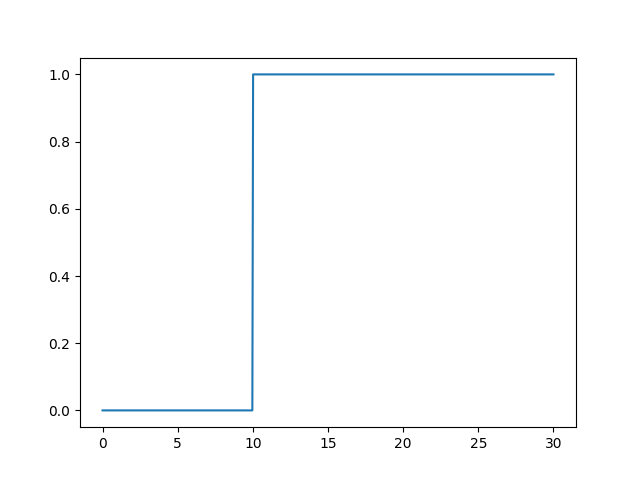
\includegraphics[scale=0.5]{images/classic_logic.png}
	\caption{``Viel größer als 1'' in der klassischen Logik}\label{class_dar}
\end{figure}

Aus der Abbildung \ref{class_dar} kann man feststellen, dass alle Werte kleiner als $10$ eine Zugehörigkeit von $0$ und solche größer oder gleich $10$ - eine Zugehörigkeit von $1$ besitzen. Diese Repräsentation entspricht jedoch die Realität nicht. Es ist eindeutig, dass $9.9$ als Wert schon größer als $1$ ist, aber der Abbildung \ref{class_dar} nach wird das nicht klar. Würde man diese Menge in der Fuzzy-Logik darstellen, ergibt sich folgende Abbildung.

% Hier Graphik f�r die Fuzzy-Set "viel gr��er als 1"
\begin{figure}[htbp]
	\centering
	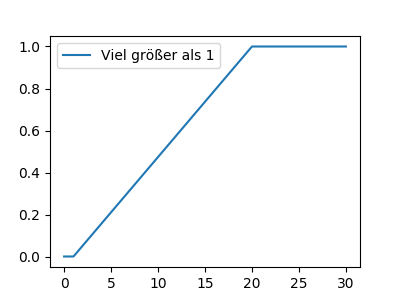
\includegraphics[scale=0.5]{images/fuzz_logic.png}
	\caption{``Viel größer als 1'' in der Fuzzy-Logik}\label{fuzzy_dar}
\end{figure}

Hier beschreibt die Ausbildung \ref{fuzzy_dar} genauer, wie die Zahlen im Vergleich zu $1$ stehen. Die Zugehörigkeit nimmt Werte zwischen $0$ und $1$. Zum Beispiel der Wert $10$ hat die Zugehörigkeit von ca. $0.5$ und für Werte größer als $20$ liefert die Funktion $\mu (x)$ einen Wert von $1$ (volle Zugehörigkeit).


\subsection{Fuzzy-Sets}\label{fs_section}%Eventuell hier beschreiben
Fuzzy-Sets, oder Fuzzy-Mengen, beschreiben in der Fuzzy-Logik Eigenschaften von Elementen. Die Idee ist, dass Elemente zu einem rationallen Wert einer Menge gehören, beziehungsweise eine Eigenschaften besitzen. In der Literatur wird folgende Definition für Fuzzy-Mengen gegeben \cite{CIKruse:15}:

\begin{definition}
	Eine Fuzzy-Menge oder Fuzzy-Teilmenge $\mu$ der Grundmenge $X$ ist eine
	Abbildung $\mu : X \rightarrow [0, 1]$, die jedem Element $x \in X$ seinen Zugehorigkeitsgrad $\mu(x)$ zu
	$\mu$ zuordnet. Die Menge aller Fuzzy-Mengen von $X$ bezeichnen wir mit $F(X)$. \cite{CIKruse:15}
\end{definition}

Mengen aus der klassischen Logik können als spezielle Fuzzy-Mengen aufgefasst werden. Also sind Fuzzy-Sets verallgemeinerte charakteristische Funktionen \cite{CIKruse:15}.

In der Praxis werden mehrere Arten von Fuzzy-Mengen entwickelt. Die bekanntesten davon sind Dreiecksfunktion, Trapezfunktion und Gaußfunktion. Ihre Namensgebung ergibt sich aus der Funktion, die sie berechnet. Drei Beispielfunktionen sind unten gegeben.

\begin{figure}[htbp]
	\centering
	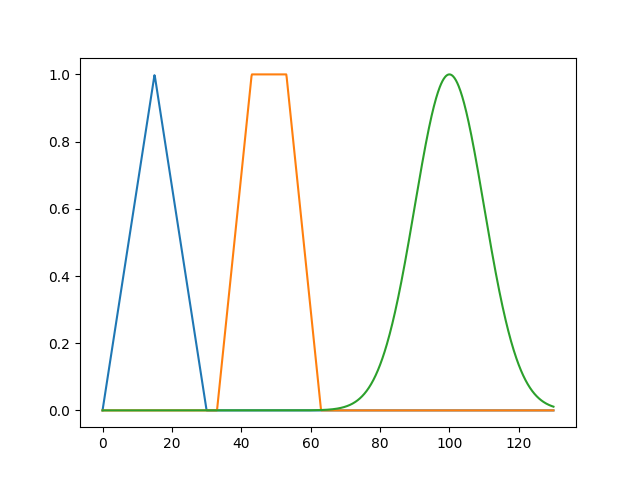
\includegraphics[scale=0.5]{images/mf_types.png}
	\caption{Dreiecks-, Trapez- und Gaußfunktion von Fuzzy-Mengen}\label{mf_types}
\end{figure}

Die Form einer Fuzzy-Menge ist durch ihre Funktion bestimmt. Die Berechnung der Dreiecksfunktion wird in \ref{dreieckfunc} .

\begin{equation}
\mu_{tri}(x) = \begin{cases}
\frac{x - a}{b - a} & \text{falls $a \leq x \leq b$}\\
\frac{c - x}{c - b} & \text{falls $b \leq x \leq c$}\\
0 & \text{sonst}
\end{cases}\label{dreieckfunc}
\end{equation}

Der Index der Funktion verdeutlicht, dass es sich um die Dreiecksfunktion handelt. Die Funktion hat drei Parametern $a, b$ und $c$, für die $a < b < c$ gelten muss. Die Dreiecksfunktion ist ein besonderer Fall der Trapezfunktion, wo die Punkte, bzw. Parametern, der oberen Grudseite gleich sind. Deswegen ist die Gleichung \ref{trap_mf} für die Trapezfunktion sehr ähnlich \cite{CIKruse:15}.

\begin{equation}
\mu_{trap}(x) = \begin{cases}
\frac{x - a}{b - a} & \text{falls $a \leq x \leq b$}\\
1 & \text{falls $b \leq x \leq c$}\\
\frac{d - x}{d - c} & \text{falls $c \leq x \leq d$}\\
0 & \text{sonst}

\label{trap_mf}
\end{cases}
\end{equation}

Die Glockefunktion ist, wie ihrer Name andeutet, eine Funktion, die die Form einer Glocke hat. Die Darstellung dieser Funktion ähnelt sich sehr der Gaußsche Funktion. Die Berechnung wird in \ref{bell_mf} gegeben. 

\begin{equation}
\mu_{bell}(x) = \frac{1}{1 + [(\frac{x - c}{a})^2]^b}
\label{bell_mf}
\end{equation}

Die letzte Funktion, die vorgestellt werden soll, ist die gaußsche Funktion. Die Formel wird öfters in der Statistik für Darstellung von Nominalverteilungen, aber auch in der Fuzzy-Logik, benutzt. Die Gaußfunktion ist in \ref{gauss_mf} gegeben \cite{CIKruse:15}:

\begin{equation}
\mu_{gauss}(x) = exp(\frac{-(x - m)^2}{s^2})
\label{gauss_mf}
\end{equation}

Die Parametern $m und q$ sind entsprechend der Mittelwert (Mittelpunkt) und die Abweichung von der Mitte, oder als $\sigma$ (Sigma) in der Statistik bekannt.




%[Fuzzy-Logik und Fuzzy-Control, Jörg Kahlert; Hubert Frank,]
%
%
%   [Fuzzy-Logik und Fuzzy-Control, Jörg Kahlert; Hubert Frank, Computational Intelligence]

\section{Operationen auf Fuzzy-Sets} \label{operatoren}
In dem vorherigen Unterkapitel \ref{fuzzy_logik} wurde die Fuzzy-Logik eingeführt, so wie auf die Repräsentation von Fuzzy-Mengen eingegangen. Um nun unscharfe Informationen verarbeiten zu können, wie Schlüsse daraus zu ziehen oder mehrere Fuzzy-Mengen zu kombinieren, brauchen wir eine Reihe von Operatoren. Da es um Mengen geht, eignen sich die Durchschnitt-, Vereinigung- und Komplementbildung aus der klassischen Logik gut. Im folgenden Kapitel werden die einzelnen Operationen beschrieben.
%\cite{} [Computational Intelligence]
\subsection{Durchscnitt}\label{AND}

In der klassischen Logik ist der Durchschnitt durch einen Logischen-UND eingesetzt. die Menge aller Elementen, die zu einer Menge $M_1$ und einer Menge $M_2$ gehören,  ist als Schnittmenge definiert. Gegeben seien die Mengen:

\begin{align}
M_1 = \{ x \ | \ x \in\Re, \ 1 \ \leq \ x \ \leq \ 3 \} 
\end{align}
\begin{align}
M_2 = \{ x \ | \ x \in\Re, \ 2 \ \leq \ x \ \leq \ 4 \} 
\end{align}

Der Durchschnitt der beiden Mengen ergibt sich aus:

\begin{align}
M_1 \cap M_2 = \{ x \ | \ x \in \Re, \ 2 \ \leq \ x \ \leq \ 3 \}
\end{align} 

Der UND-Operator lässt sich analog auf die Fuzzy-Mengen anwenden. Es wird die Fläche bestimmt, die für beide Mengen erfüllt ist. Aus methematischer Sicht sprechen wir von dem Minimum-Operator(MIN).

%\theoremstyle{definition}
\begin{definition}
	Seien $\mu_1$ und $\mu_2$ zwei Fuzzy-Mengen auf der Grundmenge $G$. Dann heißt:
	\begin{center}
		$\mu_1$ $\cap$ $\mu_2$ : $G$ $\rightarrow$ [0,1] $\text{mit}$ ($\mu_1$ $\cap$ $\mu_2$)($x$) $=$ MIN($\mu_1$($x$) , $\mu_2$($x$)) 
	\end{center}
	der \textbf{Durchschnitt} der Fuzzy-Mengen $\mu_1$ und $\mu_2$.
\end{definition} 

Zur Veranschaulichung wird unten die Grafik angegeben. Da sind zwei Fuzzy-Sets dargestellt. Die zwei Ausdrücke, die betrachtet werden, sind $mittlere$ und $hohe$ Temperatur. Der rote gestrichene Bereich stellt die Ergebnismenge dar.

\begin{figure}[htbp]
	\centering
	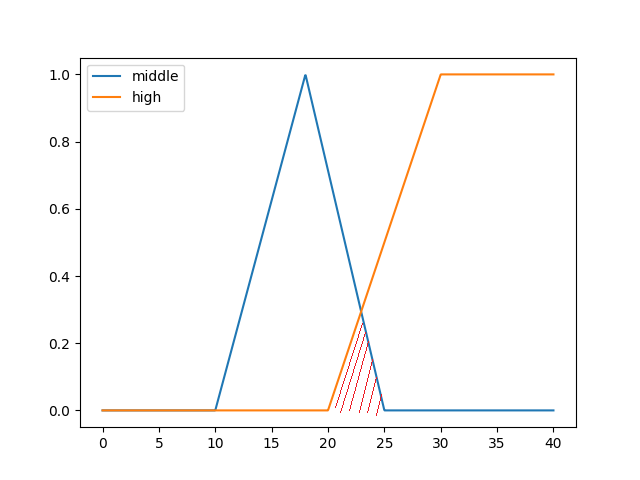
\includegraphics[scale=0.5]{images/und_high_middle_temp.png}
	\caption{Durchschnitt von zwei Fuzzy-Mengen (roter gestrichener Bereich)}\label{high_low_temp_intersection}
\end{figure}

%hier Grafik f�r die Mittlere und Hohe Temperatur mengen.


\subsection{Vereinigung}

Nehmen wir ganz einfach die Definition der Vereinigung aus der klassischen Mengenlehre:
\begin{center}
	$x$  $\in$ $M_1$ $\cup$ $M_2$ $\Leftrightarrow$ $x$ $\in$ $M_1$ $\vee$ $x$ $\in$ $M_2$
\end{center}

Ziemlich eindeutig und klar. Die Vereinigungsmenge enthält alle diese Elemente aus dem Grundbereich, die entweder in der Menge $M_1$ oder $M_2$ enthalten sind. Im nächsten Schritt wird dieser Operator an die Fuzzy-Mengen angepasst.

In der Mathematik ist dieser Operator als ODER-Verknüpfung angegeben. Die Anwendung der ODER-Operator auf Fuzzy-Mengen wird wie folgt dann definiert:

%\theoremstyle{definition}

\begin{definition}
	Seien $\mu_1$ und $\mu_2$ zwei Fuzzy-Mengen auf der Grundmenge $G$. Dann heißt:
	\begin{center}
		$\mu_1$ $\cup$ $\mu_2$ : $G$ $\rightarrow$ [0,1] $\text{mit}$  ($\mu_1$ $\cap$ $\mu_2$)($x$) $=$ $MIN$($\mu_1$($x$)), $\mu_2$($x$)) 
	\end{center}
	die $\textbf{Vereinigung}$ der Fuzzy-Mengen $\mu_1$ und $\mu_2$.
\end{definition}

Betrachten wir den selben Beispiel aus vorherigen Unterkapitel. Seien also wieder die Fuzzy-Mengen für \textit{``mittlere''} und \textit{``hohe''} Temperatur. Wenn wir den ODER-Operator auf die beiden Mengen anwenden, ergibt sich eine Ergebnismenge, die sich auf beiden Mengenflächen aufstellt. Dies wurde graphisch zunächst aufgezeichnet.

\begin{figure}[htbp]
	\centering
	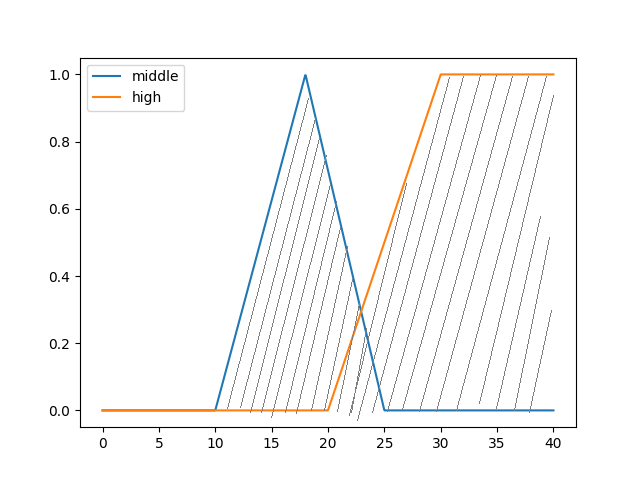
\includegraphics[scale=0.5]{images/oder_mid_high_temp.png}
	\caption{Union von Fuzzy-Mengen (gestrichener mit Blau Bereich)}
\end{figure}\label{high_low_temp_union}
% Hier Graphik f�r Oder verkn�pfung  

\subsubsection{Komplement}

Der dritte wichtige Operator ist das Komplement einer Menge. In der klassischen Mengenlehre ist dieser Operation ziemlich einfach anzuwenden. Der Operator beschreibt die Negation einer Aussage - zum Beispiel die Wahrscheinlichkeit eine 6 zu würfeln wäre $\frac{1}{6}$, die Gegenwahrscheinlichkeit, oder die Wahrscheinlichkeit etwas anderes als 6 zu würfeln wäre: (1 - $\frac{1}{6}$) = $\frac{5}{6}$. Das Komplement ist in der Fuzzy-Logik dann wie folgt definiert: 

\begin{definition}
	Sei $\mu$ eine Fuzzy-Menge auf der Grundmenge $G$. Dann heißt:
	\begin{center}
		$\mu^c$  : $G$ $\rightarrow$ [0,1] $\text{mit}$  ($\mu^c$)($x$) $=$ $1$ - $\mu$($x$)) 
	\end{center}
	die $\textbf{Vereinigung}$ der Fuzzy-Mengen $\mu_1$ und $\mu_2$.
\end{definition}

Zur Veranschaulichung die Menge \textit{hohe} Temperatur negiert. Die Negierung ist in der Graphik unten zu sehen.

%Hier Grafik f�r das Komplement-Beispiel

\begin{figure}[htbp]\label{not_high_temp}
	\centering
	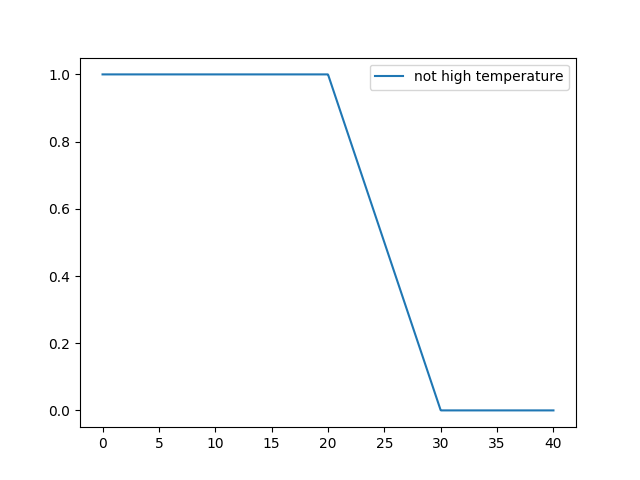
\includegraphics[scale=0.5]{images/not_high_temp.png}
	\caption{Komplement der Menge hohe Temperatur}
\end{figure}

\subsubsection{Zusammenfassung}

In diesem Unterkapitel \ref{operatoren} habe ich die drei wichtigsten Operatoren auf Fuzzy-Mengen vorgestellt. Neben den Grundverknüpfungen gibt es eine weitere Sammlung von Verknüpfungsoperatoren.

\begin{enumerate}
	\item Algebraisches Produkt: ($\mu_1$$\mu_2$) = $\mu_1$($x$) $\cdot$ $\mu_2$($x$)
	\item direkte Summe: ($\mu_1$ $\bigoplus$ $\mu_2$) = $\mu_1$($x$) + $\mu_2$(x) - $\mu_1$($x$) $\cdot$ $\mu_2$($x$)
	\item abgeschnittene Differenz: ($\mu_1$ $\sqfrowneq$ $\mu_2$) = MAX(0, $\mu_1$(x) + $\mu_2$(x) - 1)
	\item abgeschnittene Summe: ($\mu_1$ \^{+} $\mu_2$) = MIN(1, $\mu_1$(x) + $\mu_2$(x))
	\item ($\mu_1$$\dotminus$ $\mu_2$) = MIN($\mu_1$(x), 1 - $\mu_2$(x))
	\item ...
\end{enumerate}

Dies ist eine Vorbereitung auf die folgenden Kapiteln. Wir analysieren mehrere Fuzzy-Mengen und ziehen daraus bestimmte Schlüsse. Ein Beispiel dafür wäre: Wenn eine Tomate rot ist, dann ist die reif. Folgende Logische Aussagen können sehr einfach mit Fuzzy-Logic modelliert werden. In der Literatur taucht die Name Fuzzy-Regeln. Diese können dann zusammengestellt werden, um Fuzzy-Regel-Systeme aufzubauen. Das nächste Unterkapitel \ref{fuzzy_systeme} stellt Fuzzy-Systeme vor. 

\section{Fuzzy-Systeme}\label{fuzzy_systeme}

Ein Fuzzy-System, auch Fuzzy-Regler oder Fuzzy-Inferenz-System, ist ein bekannter Framework basierend auf Fuzzy-Mengen-Theorie, Fuzzy Wenn-Dann-Regeln und Fuzzy Reasoning. Konzeptionell besteht ein Fuzzy-System aus drei Grundteile - die Regelbasis, welche die Wenn-Dann-Regeln beinhaltet; die Datenbank(oder das Wörterbuch), die alle Zugehörigkeitsfunktionen definiert; und der Entscheidungmechanismus, wer die Inferenz durchführt und eine angemessene Schlussfolgerung erkundet.   

Folglich werden zwei Arten von Fuzzy-Systeme erläutert - Mamdani- und Takagi-Sugeno-Kang-Systeme.

\subsection{Mamdani-Regler}

Der Mamdani-Regler wurde im Jahr 1975 von Mamdani auf der Basis einer Veröffentlichung von Zadeh aus der Anfang der siebziger Jahren entwickelt. 

Der Mamdani-Regler ist eine endliche Menge von Wenn-Dann-Regeln $R$ der Form:
\begin{equation}
R: \text{If } x_1 \text{ is } A_1 \text{ and ... and } x_n \text{ is } A_n
\text{ then } y^\prime \text{ is } B
\end{equation}

In der Regel sind $x_1$, ..., $x_n$ die Eingangsgrößen und $y^\prime$ die Ausgabe. $A_i$ und $B$ sind  linguistischen Werte. Jede Regel besteht aus zwei Teilen - Prämissen und Konklusionen. Jede Vorbedingung untersucht spezifische Eigenschaften. Es wird geprüft, ob der Eingangwert diese Eigenschaften erfüllt. Anhand diese Merkmale schließt sich eine Konklusion. 

Sei $W$ die Menge aller linguistischen Konklusionen $B_i$, so dass $B_1, \dots, B_m \in W$ gilt. Der Regler kann als eine n-Stellige Funktion mit $f: \mathbb{G^n} \mapsto W$ dargestellt werden. Die Funktion ordnet eine Eingabe zu einem linguistischen Term $B_i$.

\begin{equation}
f(x_1, ..., x_n) \approx 
\left\{
\begin{array}{ll}
B_1 & \mbox{ falls } x_1 \mbox{ is } A_1^{(1)} \mbox{ und ..., und } x_{n} \mbox{ is } A_n^{(1)}\\
\vdots \\
B_{m} & \mbox{ falls } x_1 \mbox{ is } A_1^{(m)} \mbox{ und ... und } x_{n} \mbox{ is } A_n^{(m)}
\end{array}
\right.
\end{equation}

In der Funktion gibt es genau so viele Ausgaben, wie es Regeln gibt - $m$.

Mit einem Mamdani-Regler können viele Probleme aus der reellen Welt definiert werden. Als kleines Beispiel eignet sich die Farben der Tomaten. Wir betrachten die Farbe als Eingabe. Die Ausgabe würde uns sagen, wie reif eine Tomate ist. Wir teilen unsere Eingangsgrößen in drei Farben: rot, gelb und grün. Daraus lassen sich entsprechend 3 Fuzzy-Mengen definieren. Als Ausgabe wird die Reife einer Tomate bestimmt. Das Ergebnis kann in drei Mengen anfallen: reif, halbreif oder unreif. Auf dieser Weise haben wir ein Mamdani-Fuzzy-Model, das aus 3 Fuzzy-Sets und aus 3 Regeln besteht. Die Regelbasis sieht wie folgt aus:

\begin{itemize}
	\item $R_1$: if x is rot, then y is reif.
	\item $R_2$: if x is gelb, then y is halbreif.
	\item $R_3$: if x is grün, then y is unreif.
\end{itemize}

Eine Tabelle für die Fuzzy-Relationen ist unten gegeben

\begin{table}\label{tomato:1}
	\centering
	\begin{tabular}{c|c c c}
		
		x \diagdown \ y & \ unreif & \ halbreif & \ reif \\ [0.5ex]
		\hline
		grün & 1 & 0 & 0 \\ 
		gelb & 0 & 1 & 0\\
		rot  & 0 & 0 & 1\\
		
	\end{tabular}
	\caption{Beispiel für Tomaten}
	
\end{table}

Wie man sieht die Tabelle ist ziemlich einfach zu lesen, wenn die Tomate grün ist, wird immer angenommen dass sie unreif ist. Man könnte entsprechend die Fuzzy-Mengen aus der Konklusion verfeinern. Das würde bedeuten, dass die Mengen sich überlappen. Unsere Tabelle könnte dann wie Tabelle \ref{table:1} aussehen:

\begin{table}
	\centering
	\begin{tabular}{c|c c c}
		
		x \diagdown \ y & \ unreif & \ halbreif & \ reif \\ [0.5ex]
		\hline
		grün & 1 & 0.5 & 0 \\ 
		gelb & 0.3 & 1 & 0.3\\
		rot  & 0 & 0.5 & 1\\
		
	\end{tabular}
	\caption{Beispiel für Tomaten}
	\label{table:1}
\end{table}

Abhängig davon wie man die Ausgangsmengen definiert, wie weit die Mengen überlappen, ergibt sich eine unterschiedliche Interpretation der Werte. Je mehr Fuzzy-Sets für eine Größe(Maß) definiert sind, desto besser könnte ihr Zustand repräsentiert werden. Mit der Anzahl der Fuzzy-Sets steigt die Komplexität eines Systems proportional.

Den oberen kleinen Beispiel zeigt wie einfach Mamdani-Modelle zu modellieren sind. Mamdani-Reglern finden in der Praxis öfters Einsetzung.

\section{Takagi-Sugeno-Kang-Modell} \label{TSK}

Das Takagi-Sugeno-Kang-Modell ist dem Mamdani-Modell sehr ähnlich. Der Unterschied erweist sich in der Konklusion. TSK-Regler verwenden Regeln der Form:

\begin{align}
R: \text{ If } x_1 \text{ is } \mu_R^{(1)} \text{ and \ldots and } x_n \text{ is } \mu_R^{(n)} \text{ then } y = f_R(x_1,\ldots,x_n).
\end{align}}

In den Prämissen der beiden Fuzzy-Systeme liegt kein Unterschied. Die Besonderheit des TSK-Modells liegt in der Konklusion. Da steht eine lineare Funktion, anstatt eine Fuzzy-Menge. In der Konklusion kann jede beliebige Funktion $f$ mit belibiger Eingabe berechnet werden. Die Form der linearen Funktion ist in \ref{lin_func} gegeben:
\begin{align}
f(x_1, \ldots, x_n) = p_0 + p_1\cdot x_1 + \ldots + p_n\cdot x_n,
\label{lin_func}
\end{align}
$p_0, \ldots, p_n$ sind die Parametern der Konklusionsfunktion. Für geeignet ausgewählte Parameterwerte beschreibt das TSK-Modell eine belibige mathematische Funktion, dies kann z.B. die Quadratfunktion sein. Für den Fall, dass die Parametern $p_1, \ldots p_n$ den Wert 0 haben, erhält man einen Mamdani-Modell mit scharfer Ausgabe. Solche Modelle heißen in der Literatur auch \textbf{zero-order Sugeno-Fuzzy-Modelle} \cite{SCTemassi:01, NFMBothe:98, NFSC:97}.
Als Beispiel kann folgende Regelbasis betrachtet werden:
\begin{align*}
&R_1: \text{ If } x \text{ is ``sehr klein'' then } y = 0\\
&R_2: \text{ If } x \text{ is ``klein'' then } y = 1\\
&R_3: \text{ If } x \text{ is ``groß'' then } y = 2\\
&R_4: \text{ If } x \text{ is ``sehr groß'' then } y = 3. \\
\end{align*}
Die Fuzzy-Sets sind ``sehr klein'', ``klein'', ``groß'' und ``sehr groß'' und die Ergebnisswerte entsprechend \textit{0, 1, 2 und 3}.

\subsubsection{Fuzzifizierung und Defuzzifizierung}\label{FDF} 

Der Vorgang eines Modells zerlegt sich in zwei Teilen - Fuzzifizierung und Defuzzifizierung. Der erste Begriff beschreibt den Prozess für die Evaluierung der Eingangswerte in Fuzzyinferenzsysteme. Es gibt mehrere Evaluierungsmethoden, beziehungsweise Fuzzifizierungsmechanismen, wie zum Beispiel die Gaußsche Funktion (\ref{fs_section}). Der zweite Begriff bezeichnet die Vorgehensweise bei der Berechnung der Ausgabe, oder Inferenz, eines Fuzzy-Systems. Die Reihenfolge der beiden Prozesse ist somit bestimmt. Da im vorrigen Kapitel schon Beispiele für Fuzzifizierungsverfahren vorgestellt werden, wird demnächst in den unterschiedlichen Arten von Defuzzifizierung eingestiegen.

Bei der Regelaktivierung unterscheidet man zwei Fällen. Wenn die Eingabe eine volle Zugehörigkeit zu einer Fuzzy-Menge ergibt, dann liefert das Modell ganz normal den Wert der entsprechenden Konklusionsfunktion. Bei partielle Aktivierung mehreren Regeln ergibt sich das Inferenzergebnis aus einem spezifischen Verfahren. Dafür werden bestimmte Inferenzmethoden angewendet, zum Beispiel das Center of Gravity, oder Center of Area. Einige dieser Methoden werden inden folgenden Unterkapiteln vorgestellt. In allen Verfahren handelt es sich, um Mamdani-Reglern, wo die Konklusion einer Regel aus einer Fuzzy-Mengen besteht. Die letzte vorgestellte Methode ist spezifisch für Takagi-Sugeno-Kang-Modelle anzuwenden.

\subsubsection{Height Method}
Bei dieser Methode, auch als \textit{maximum membership principle} bekannt, wird der Regelaktievierung mit den größten Wert ausgewählt. Die Vorgehensweise könnte in Systeme verwendet werden, wo der größte Zutreffer nur wichtig ist. Als Beispiel könnte ein System mit entsprechenden Gegenmaßnahmen genannt werden, wo der größte Risiko Vorgang haben soll \cite{SCTemassi:01}.

\subsubsection{Center of Gravity}

Center of Gravity, auch als Center of Area bekannt, ist die prominenteste Methode von allen, wo sich das Ergebniss als schärfer Wert ergibt. Das Endergebniss berechnet sich aus folgender Formel:
\begin{align}
y^* = \frac{\int y \cdot \mu_R(y)dy}{\int \mu_R(y)dy}
\end{align}

Der Wert \textit{y} hier ist das Ergebnis der aktivierte Regel \textit{R} und \textit{$y^*$} ist das Endergebniss. \cite{SCTemassi:01}

\subsubsection{Weighted Average Method}

Die gewichtete Durchschnittsmethode, oder Weighted Average Method, ist nur für Ausgangszugehörigkeitsfunktionen, die aus mehreren symmetrischen Zugehörigkeitsfunktionen $\mu_i$ besteht. Die Formel lautet:

\begin{align}
	y^* = \frac{\sum_{i} \=y \cdot \mu_i(\=y)}{\sum \mu_i(\=y)}
\end{align}

Das Modus jeder Zugehörigkeitsfunktion $\mu_i$ wird durch den Wert von $\=y$ beschrieben. \cite{SCTemassi:01}

\subsubsection{Takagi-Sugeno-Kang-Defuzzifizierungsmethode}
Die Defuzzifizierungsmethode von TSK-Modelle berechnet eine Interpolation zwischen den Ausgangswerten. Das Endergebnis ergibt sich aus dem Ausgabewert jeder Regel und dessen Multilizierung mit dem Gewicht der entsprechenden Regel und geteilt durch die Summe der Wahrheitsrate jeder Regel. Die Formel ist gegeben:
\begin{align}\label{TSK_defuzz}
y = \frac{\sum_{i} \mu_i \cdot f_i(x_1, ..., x_n)}{\sum \mu_i},
\end{align} wo $\mu_i$ die Wahrheitsrate, bzw. Aktievierungswert, einer Regel $i$ ist und $f_i$ liefert den Ergebniswert für die Regel bei Eingabe $x_1, ..., x_n$.

Zum Schluss wird eine Abbildung gegeben, die den gesammten Prozess, Fuzzifizierung und Defuzzifizierung, darstellt. Die Abbildung \ref{TSK_Modell} beschreibt, wie das Endergebnis berechnet wird.

\begin{figure}[htbp]
\centering
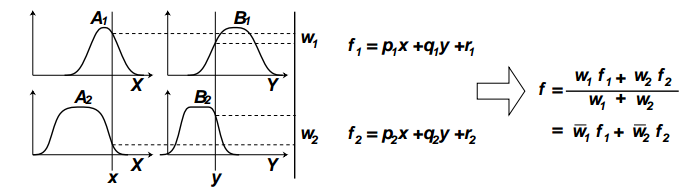
\includegraphics[scale=0.5]{images/TSK_Modell.png}
\caption{Inferenzschritt eines TSK-Modells \cite{Jang:93}}\label{TSK_Modell}
\end{figure}

In der Abbildung \ref{TSK_Modell} wird ein Model mit zwei Eingangsgrößen und zwei Fuzzy-Mengen pro Eingabe dargestellt. Die Regelbasis besteht aus zwei Regeln. Die Fuzzy-Mengen werden durch die Glockenfunktion berechnet. Die Variablen $w_1$ und $w_2$ liefern die Regelaktievierungen für die Regeln mit entsprechenden Indexen. Das Endergebnis ergibt sich aus der oben definierten Funktion \ref{TSK_defuzz}.

%Unsicher ob ich darauf eingehen soll

%Die Gliederung h�ngt nat�rlich vom Thema und von der L�sungsstrategie ab. Als n�tzliche
%Anhaltspunkte k�nnen die Entwicklungsstufen oder - schritte z.B. der Softwareentwicklung betrachtet werden. N�tzliche Gesichtspunkte erh�lt und erkennt man, wenn man sich
%\begin{itemize}
%  \item in die Rolle des Lesers oder
%  \item in die Rolle des Entwicklers, der die Arbeit z.B. fortsetzen, erg�nzen oder pflegen soll,
%\end{itemize}
%versetzt. In der Regel wird vorausgesetzt, dass die Leser einen fachlichen Hintergrund haben - z.B. Informatik studiert haben. D.h. nur in besonderen, abgesprochenen F�llen schreibt man in popul�rer Sprache, so dass auch Nicht-Fachleute die Ausarbeitung prinzipiell lesen und verstehen k�nnen.
%
%Die �u�ere Gestaltung der Ausarbeitung hinsichtlich Abschnittformate, Abbildungen, mathematische Formeln usw. wird in \hyperref[Stile]{Kapitel~\ref*{Stile}} kurz dargestellt.











%% KI Kapitel
\section{Künstliche Neuronale Netze} \label{ANN}

Künstliche Neuronale Netze (engl. artificial neural networks) sind Systeme, die auf dem Gehirn von Tieren und Menschen basieren und besteht aus endlich viele Einheiten, Neuronen. Der Datenaustausch geschieht über gerichtete Verbindungen zwischen den Neuronen. Forscher beschäftigen sich mit Neuronalen Netzen aus unterschiedlichen Gründen. In der Biologie simulieren Forscher diese, um sich den Prozess des Lernens und weitere Mechaniscmen zu untersuchen. In der Informatik wird aber versucht, die Lernfähigkeit des Gehirns nachzubilden und auszunutzen.

In den folgenden Kapiteln wird zuerst auf den Neuronen sowohl in der Biologie als auch in der Künstliche Intelligen eingegangen. Weiterhin werden die Eigenschaften von Neuronalen Netzen erklärt. Zum Schluss stelle ich den Gradientenvarfahren vor, anhand dessen diese Netze lernen.

\section{Biologische Grundlagen}

Das tierische Gehirn leitet jede einzelne Aktivität in dem Körper eines Tieres, inklusive die Verarbeitung von Daten. Laut \cite{GEHIRN:12} besteht das Gehirn aus 86 Milliarden Neuronen, die in Cliquen verbunden sind. Neuronen in einer Clique komunizieren untereinander, indem sie Signale über ihre Axone weiterleiten und Signale über ihren Dendrit empfangen. Eine Verbindung zwischen Neuronen existiert, wenn die Axonterminale eines Neurons den Dendrit eines anderen berührt. Zur Veranschaulichung ist den Aufbau eines Neurons in Abbildung \ref{neuron} gegeben. Jeder Signal wird in dem Soma verarbeitet und durch die Axone weitergeschickt.

\begin{figure}[!htbp]
	\centering
	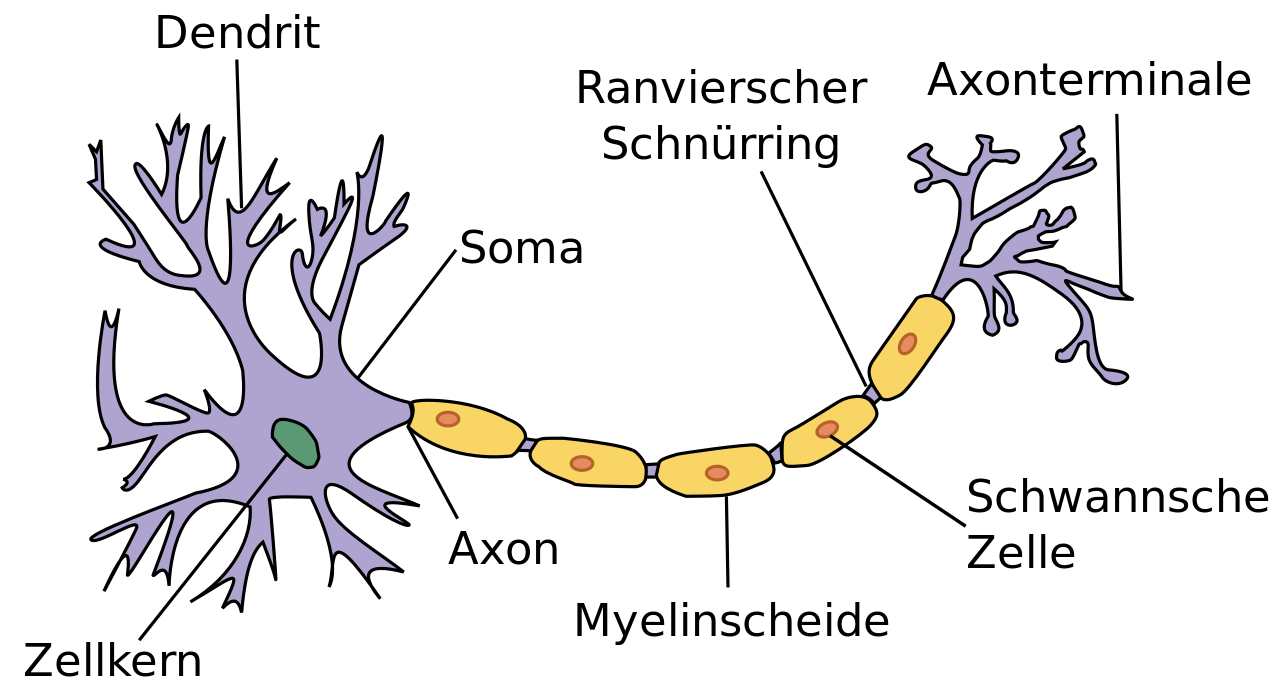
\includegraphics[scale=0.2]{images/Neuron_(deutsch)-1.png}
	\caption{Neuron \cite{NWIKI:19}}\label{neuron}
\end{figure}

Auf dem selben Prinzip funktionieren auch Neuronen in Künstlichen Neuronalen Netzen (KNN). Im folgenden Kapitel wird mehr darauf eingegangen. \cite{NWIKI:19} \cite{GEHIRN:12}

\subsection{Neuron in Künstlichen Neuronalen Netzen}

Neuronale Netze sind streng genommen gerichtete Graphen, wo jeder Knoten ein Neuron ist und jede Kante eine Verbindung zwischen Neuronen beschreibt. Die Neuronen können in drei Gruppen, oder auch als Schichten (\textit{engl.} Layers) bekannt, unterteilt werden - Eingabe-, Ausgabe- und versteckte Neuronen. Die Ein- und Ausgabeknoten sind die Einheiten, die mit der Umgebung verbunden sind, dabei ist klar welche Knoten was sind. Die übrigen Elemente werden in dem Netz eingebaut und kommunizieren nur mit anderen Neuronen. Daraus ergibt sich auch ihren Namen ``versteckt''.

Jede Verbindung zwischen Neuronen in KNN erhält ein Wert. Der Verbindungswert wird meistens als Gewicht bekannt. Bei einem Gewicht von 0 existiert keine Verbindung zwischen Neuronen. In einem KNN werden nur die Gewichte gelernt, während die Neuronen nur eine mathematische Funktion beschreiben. Eine übliche Repräsentation der Gewichte ist die Matrix \ref{knnmat}.

\begin{align}
\centering
\bordermatrix{ 	
	& u_1 			& u_2			 & \dots & u_r			    \cr
	u_1    & w_{u_{1}u_{1}} & w_{u_{1}u_{2}} & \dots & w_{u_{1}u_r}		\cr
	u_2	   & w_{u_{2}u_{1}} & w_{u_{2}u_{1}} & 	     & w_{u_{2}u_{1}}	\cr
	\vdots & \vdots	      	& 			     &       & \vdots			\cr
	u_r    & w_{u_{r}u_{1}} & w_{u_{r}u_{2}} & \dots & w_{u_{r}u_r}  	\cr 
}
\label{knnmat}
\end{align}

Die Beziehungen zwischen Neuronen aus zwei Schichten wird außerdem ganz gut in der Matrix dargestellt. Sie ist von oben nach rechts zu lesen, also die Spalten sind es dem Neuronen zugeordnet, aus denen die Verbindungen ausgehen. Das heißt der Knoten $u_1$ hat eine Verbindung zu sich selbst und dem Neuron $u_2$ und die Gewichtwerte sind entsprechend $w_{u_{1}u_{1}}$ und $w_{u_{1}u_{2}}$. Die Darstellung als Matrix erlaubt es alle mathematischen Operationen durchzuführen, indem der Ausgabe eines Neurons, oder die Eingabe aus der Umgebung, rechts an der Matrix dranmultipliziert. \cite{CIKruse:15} \cite{NFMBothe:98} \cite{SCTemassi:01} \cite{CISCNFI:98}

\section{Lernen} % s. 58 Book 2; s.40 Computational Intelligence s. 21
Die erstaunlichste Eigenschaft Neuronaler Netze ist ihre Möglichkeit, eine Aufgabe, bzw. Fähigkeit, zu erlernen. Gewichtswerte und/oder weitere Parameter unterliegt Änderungen nach jeder Iterationsschritt während des Lernprozesses. In Bezug auf dem Iterationsschritt wird es zwischen ``Offline-'' und ``Onlinelernen'' unterschieden. Außerdem unterscheidet man zwei weiteren Gruppen in der Lernmethode eines Neuronalen Netzes - überwachtes (\textit{engl.} supervised) und unüberwachtes (\textit{engl.} unsupervised) Lernen. Demnächst werden die Begriffe einzeln untersucht. Danach werden nur beaufsichtigte Algorithmen vorgestellt, da die relevant für mein Projekt sind. Zum Schluss werden die Offline- und Online-Lernverfahren vorgestellt, die insgesammt drei sind.  \cite{SCTemassi:01} \cite{CIKruse:15} \cite{NFSC:97} %Nach jedem Schritt können Gewichtswerte und/oder weitere Parameter optimiert werden.

\subsection{Unsupervised Learning}
Unsupervised Learning (\textit{deutsch} unbeaufsichtigtes Lernen) besteht immer noch eine Ein-/Ausgabe beziehung, jedoch wird kein Fehlerfunktion eingesetzt. In diesem Fall muss das Netz Mustern aus den Ein-/Ausgabepaare erkennen und zusammengruppieren.

\subsection{Supervised Learning}

Unter Supervised Learning versteht man den Verfahren, bei dem das Netz anahand von Ein-/Ausgabepaare trainiert wird. Das Lernenprozess beinhaltet die allmäliche Anpassung der Gewichtparametern bei jedem Iterationsschritt, so dass bei gegebener Eingabe $x$ der Fehler, der aus der Ausgabe und dem Erwartungswert berechnet wird, minimiert wird. Die Fehlerfunktion wird in vielen Fällen auch als ``Kritiker'' und das Modell als ``Kritisierender'' bekannt. Ein Speziallfall des überwachtes Lernen ist ``reinforcement Learning''. In dem Lernverfahren wird jede Berechnung ``richtig'' oder ``falsch'' bewertet, ohne dass ein Fehler unbedingt berechnet wird. \cite{SCTemassi:01} \cite{CIKruse:15} \cite{NFSC:97}

\subsubsection{Least Mean Square Method}
Die Kleinste Quadrate Methode (\textit{engl.} Least Mean Square Method) wurde von den B. Widrow und M.Hoff für ein Projekt namens ADALINE oder ADAptive LINear Element entwickelt. Die Methode versucht die Fehlerrate mit dem Gradientenverfahren zu verringern. Die Fehlerrate wird mit dem Mean Squared Error (MSE) geteilt durch die Anzahl der Elementen im Trainingsdaten berechnet. Die Formel ist gegeben:

\begin{align}
E(w) = \frac{1}{2} \sum_{i=1}^{m}(d_i - y_i)^2 \label{MSE}, 
\end{align}

wobei $w$ ist der Gewichtsvektor, und $d_i$ und $y_i$ entsprechend - Erwartungs- und Ausgabewert. Die Ableitung der Funktion ergibt den nächsten Iterationsschritt:

\begin{align}
w^{t+1} = w^t + \mu(d_k^t - y_k^t)x_k^t.
\end{align}

Die Konstante $\mu$ kontrolliert die Konvergenz und Stabilität, \textbf{w} und textbf{x} sind Gewichtsvektor und Eingabe. Der Schritt wird durch den Exponent $t$ bestimmt - $t+1$ ist der nächste Schritt. Solange die Konstante entsprechend gewählt wird, konvergiert der Verfahren und der gesuchte Gewichtvektor kann gelernt werden. \cite{SCTemassi:01}

\subsubsection{Backpropagation Algorithm}
Der Backpropagation Algorithmus, oder auch als Gradient Descent bekannt, wurde laut \cite{SCTemassi:01} am Ende der 70er Jahren von Paul J. Warbos entwickelt. Dieses Verfahren hat die Interesse an Neuronalen Netzen wiederbelebt.

Der Algorithmus ist der bekannteste Lernalgorithmus für beaufsichtigtes Lernen. In dem Verfahren stecken zwei wichtige Konzepte. Zum einen liegt der Feedforwardphase vor, die dann folgendes Verhalten beschreibt: die Eingabe-/Erwartungswerte dem Neuronalen Netz gegeben werden und anschließend eine Ausgabe berechnet wird. Danach wird der Fehler berechnet, für den eine bestimmte Fehlerfunktion verwendet wird, z.B. der Mean Squared Error (siehe Gleichung \ref{MSE}). In der zweiten Phase, auch Rückwertsphase genannt, werden die Knoten rückwerts anfangend von der Ausgabe- über die versteckten Schichten bis zum Eingabeschicht angepasst. Das Ziel der Rückwertsschritt ist es den Fehlre zu minimieren. Hinter dem Verfahren stecken einfache Mathematische Operationen, wurde aber in dieser Ausarbeitung nicht betrachtet. In dem Buch \cite{SCTemassi:01} wird jedoch eine sehr ausführliche Beschreibung des Algorithmus in Schritten angegeben, welche auch hier figuriert.

\begin{enumerate}\label{BPA}
	\item Die Gewichte werden zufällig initialisiert.
	\item Eine Ein-/Ausgabe paar wird dem Netz vorgestellt.
	\item Liefer die Ausgabe des Netzes.
	\item Berechne die Fehlerrate (z.B. durch die Mean Squared Error \ref{MSE}).
	\item Beginnend mit der letzten Schicht berechne den Wert der Ableitung $\delta_j$ rückwerts.
	\item Passe die Gewichte nach in dem Netz.
	\item Wiederhole ab 2. Schritt für angegebene Anzahl an Iterationen, oder bis die Fehlerrate kleiner als ein Betrag wird.
\end{enumerate}

% Hier das Algorithmus, wie es im Buch figuriert, angeben

\subsection{Schlüsse}

Es werden zwei Bibliotheken für Neuronale Netze berücksichtigt - Tensorflow und SciKit. Biobliotheken sind in der Regel sehr ähnlich. In diesem Fall bieten die betrachteten APIs die nötigten Funktionalitäten, um das Projekt umzusetzen. Jedoch das Ursprüngliche Gedacht war, dass ich die erstellten Neuronalen Modelle in C++ exportiere. Das würde erfordern, dass eventuell das ANFIS-Model mit Hilfe von andere Bibliotheken gegenüber C++ kompilieren müsste. Der Grund, warum ich dann zu Tensorflow geneigt habe, ist, weil Tensorflow geschriebene Modelle, einfach in Dateien zu exportieren sind. Was wiederum mich erlaubt das Model in C++ ohne weiteres zu importieren.

%% Neuro Fuzzy








\section{Neuro-Fuzzy-Systeme}

Im vorletzten Kapitel wurden zwei Arten von Fuzzy-Systeme, oder Reglern, vorgestellt. Solche Systeme werden in der Praxis öfters mit Konzepte aus der Künstliche Intelligenz kombiniert. Zum einen bietet sich Kombinationen mit Neural Networks \ref{ANN}, Evolutionäralgorithmen und vielen weiteren. Im folgenden Kapitel wird besonders die Kombination mit Neuronalen Netzen untersucht. Die Zusammenarbeit von Fuzzy-Reglern und Neuronalen Netzen ist atraktiv, weil die Interpretierbarkeit von Fuzzy-Systeme mit den Lernmöglichkeit von Neuronalen Netzen effektiv zu verbinden ist. In den nächsten Unterkapiteln werden zwei Arten von Modelle mit jeweils einer Beispielstruktur - Modelle für feste Lernaufgaben und solche mit verstärkendem Lernen. Die Modelle werden außerdem in der Literatur als Neuro-Fuzzy-Systeme, bzw. Neuro-Fuzzy-Regler, bezeichnet. \cite{CIKruse:15}
\section{Neuro-Fuzzy-Regler}

Neuro-Fuzzy-Regler, oder Neuro-Fuzzy-Systeme, sind Modelle, bei denen konzeptionelle Teile von Neuronalen Netzen und Fuzzy-Systeme kombiniert werden. Das Ziel dieser Reglern ist es das beste aus beiden Welten zu kombinieren - Lernbarkeit von Neuronalen Netzen und Interpretierbarkeit von Fuzzy-Systeme. Außerdem bietet Fuzzy-Systeme die Möglichkeit Vorwissen einzubrigen, was hingegen die Lernzeit der Neuronalen Netze verkürzt. Am Ende des Lernprozesses erhält man ein Modell, dessen Regelungsstragie interpretierbar ist und dessen Regelung überprüft und eventuell noch angepasst werden können \cite{CIKruse:15}. Demnächst werden zwei Arten von Neuro-Fuzzy-Modelle, die unterschiedliche Anwendungsfälle haben.

\subsection{Modell f\"{u}r feste Lernaufgaben}
%(Muss Änderungen unterliegen)

Neuro-Fuzzy-Modell für feste Lernaufgaben versuchen, Fuzzy-Mengen und, bei TSK-Modelln, die Parameter der Ausgabefunktion unter Einreichung einer Mengen von Ein-/Ausgabe-Tupeln zu optimieren. Diese Modell sind genau dann sinnvoll, wenn schon eine Fuzzy-Regelbasis vorliegt. Die Regelbasis unterliegt infolge des Lernens eine Verarbeitung, die als Ziel eine Optimierung hat. %Dafür sind geieignete Ein-/Ausgabedaten gebraucht.

Ein weiteres Anwendungsbeispiel ist bei bereits existierender Regelbasis, dass dieser mit einer neuen ausgetauscht wird. Falls die Basis schon errechnete Werte geliefert hat, können diese zusammen mit den zugehörigen Eingabewerten dem Neuro-Fuzzy-System zum Lernen gegeben werden. Am Ende erhält man eine optimierte Fuzzy-Regel-Basis, die die alte Basis ``ersetzt''.

Falls es keine angemessene Lernaufgabe bereits gegeben ist, dann eignet sich dieses Verfahren nicht. Es existieren natürlich Ansätze, die es ermöglichen, einen initialen Regelbasis aus Eingabedaten zu erstellen. Ein solcher Verfahren wird später noch vorgestellt.

Folglich wird ein Beispiel von einem Modell, das sich für feste Lernaufgaben eignet, vorgestellt. Es geht nämlich um das ANFIS-Modell.

\subsubsection{Das ANFIS-Modell}

Im Frühjahr von 1993 wurde das Neuro-Fuzzy-System ANFIS (Adaptive Neuro-Fuzzy Inference System oder Adaptive Network-based Fuzzy Inference System) entwickelt. Das Modell wurde in mehrere Software-Pakete schon eingesetzt. Die ANFIS basiert auf einer hybriden Struktur, sodass es sowohl als ein Neuronales Netz, als auch als ein Fuzzy-System interpretiert werden kann. In dem System sind Regeln angelegt, die nach dem TSK-Modell definiert sind (Takagi-Sugeno-Kang-Reglern \ref{TSK}). Die Abbildung \ref{ANFIS_Abb} zeigt einen Modell mit folgender Regelbasis:%(Abbildung hier zitieren aus Buch 2)

\begin{minipage}{\textwidth}

\begin{center}
	$\newline$
	$R_1$: Falls $x_1$ ist $A_1$ und $x_2$ ist $B_1$, dann ist $y$=$f_1$($x_1$,$x_2$)\\
	
	$R_2$: Falls $x_1$ ist $A_1$ und $x_2$ ist $B_2$, dann ist $y$=$f_2$($x_1$,$x_2$)\\
	
	$R_3$: Falls $x_1$ ist $A_2$ und $x_2$ ist $B_2$, dann ist $y$=$f_3$($x_1$,$x_2$),
\end{center}
\end{minipage}
dabei sind $A_1$, $A_2$, $B_1$ und $B_2$ linguistische Termen, die den entsprechenden Fuzzy-Mengen $\mu_i^{(j)}$ zugeordnet sind. Die Funktionen $f_i$ sind linear und sehen wie folgt aus (siehe \ref{FDF}):
\begin{equation}
f_i(x_1, x_2) = p_0^{i} + p_1^{i}\cdot x_1 + p_2^{i}\cdot x_2
\end{equation}

Der Konklusionsfunktion $f_i$ entspricht die Regel $R_i$. Somit hat jede Regel eine eindeutige Ausgangsfunktionen mit eindeutigen Parametern $p_0^{i}, p_1^{i}, p_2^{i}$.

Die Ausgabe eines ANFIS-Modells berechnet sich genau so wie ein TSK-Modell (siehe \ref{FDF}). %Zuerst wird der Zugehörigkeitsgrad einer Regel mit dem entsprechenden Konklusionsfunktion multipliziert. WeiterhinAnschließend normiert man das Resultat  summiert man das Resultat aus allen Regeln und teilt die Summe durch die Summe aller Anktivierungsgraden. 
Für den genannten Beispiel lautet die Ausgabe:
\begin{align}
f = \dfrac{\sum_{i}^{3} \tilde{w_i}\cdot f_i(x_1, x_2)}{\sum_{i}^{3} \tilde{w_i}}
\end{align}

Der ANFIS-Ansatz besteht aus 5 Schichten. Die Abbildung \ref{ANFIS_Abb} veranschaulicht die Struktur.

\begin{figure}[htbp]
	\centering
	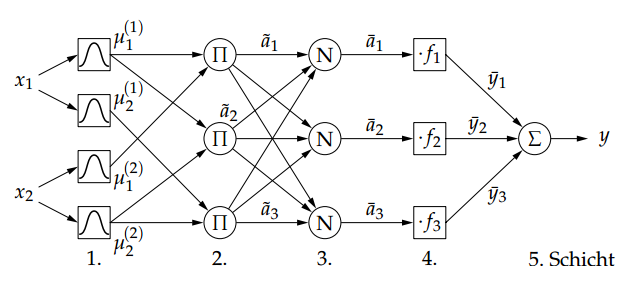
\includegraphics[scale=0.5]{images/ANFIS_Abb.png}
	\caption{ANFIS-Model \cite{CIKruse:15}}\label{ANFIS_Abb}
\end{figure}

In der \textbf{ersten Schicht} werden die Eingabewerte eingereicht und entsprechend die Zugehörigkeiten zu den Fuzzy-Sets ausgegeben. Weiterhin werden in der \textbf{zweiten Schicht} die Aktivierungswerte jeder Regel ausgewertet. Die Neuronen werden mit $\prod$ gekennzeichnet. Einzelnen Fuzzyzugehörigkeitswerte werden mittels Operatoren kombiniert, um die Aktivierungsgrad jeder Regel zu berechnen. Hier dürfen Operatoren zur Verknüpfung von Fuzzy-Mengen eingesetzt werden, üblicherweise der UND-Operator (siehe \ref{AND}). Die Gleichung \ref{eq3_3} ergibt die Berechnung bei gegebener UND-Verknüpfung:

\begin{equation}\label{eq3_3}
\tilde{w}_i = \prod \mu_i^j(x_j)
\end{equation}

Die Variable $\tilde{w}_i$ ergibt die Aktivierung, oder Erf\"{u}llungsgrad, des Regels $R_i$ und $\mu_i^j$ ist die $j.$ Zugehörigkeitsfunktion in der Regel $R_i$.

Im \textbf{dritten Schicht} findet die Normalisierung aller Aktivierungswerte $\tilde{w}_i$ statt. Mit einfachen Worten wird der Beitrag berechnet, den jeder Regel für den Gesamtausgabe beiträgt. Nach der Normalisierung erhält man Aktivierungsgrößen zwischen $0$ und $1$. Die Gleichung \ref{barwi} berechnet die normalisierten Werten für jeden Regel $R_i$:

\begin{equation}\label{barwi}
\bar{w}_i = \frac{\tilde{w}_i }{\sum_j \tilde{w}_j } 
\end{equation}

Im \textbf{vierten Schicht} berechnen die mit $N$ markierten Neuronen die gewichteten Ausgabewerte. Das ``Gewicht'' (Ergebnis) aus dem letzten Layer wird mit der entsprechenden Ausgabefunktion multipliziert:

\begin{equation}
\bar{y}_i = net_i = \bar{w}_i\cdot f_i(x_1, ..., x_n). 
\end{equation}

Im \textbf{fünften Schicht} steht ein einziges Neuron, der mit $\sum$ beschriftet ist. Im letzten Schicht berechet man die Ausgabe, indem alle Werte aus dem \textbf{vierten Schicht} zusammenaddiert werden:

\begin{equation}
y = y_{out} = \sum_i \bar{y}_i = \frac{\tilde{w}_i\cdot f_i(x_1, ..., x_n)}{\sum_j \tilde{w}_j}.
\end{equation}

Diese Struktur ähnelt sich der von TSK-Modell. Für die Optimierung von Parametern der Zugehörigkeitsfunktionen und Konklusionsfunktionen eignet sich der ANFIS-Ansatz.

Das ANFIS-Modell ermöglicht die Optimierung von Modellparametern - die Fuzzy-Mengen- und Ausgabefunktionsparametern. Diese können erlernt werden, wenn eine angemessene Lernaufgabe vorliegt. Außerdem muss eine ausreichende Menge von Ein-/Ausgabe-Werten zur Verfügung stehen. Es bieten sich mehrere Lernmethoden zur Optimierung der Parametern. Zwei davon sind Gradientenverfahren(analog zur Fehler-Rückpropagation-Verfahren aus Neuronalen Netzen) und die Kleinste-Quadrate-Methode. \cite{CIKruse:15} \cite{Jang:93}

\subsection{Modell mit verstärkendem Lernen}

Bei Modellen mit verstärkendem Lernen wird versucht, die Menge der Daten für das Lernen möglichst gering zu halten. Der Unterschied zwischen Modell mit verstärkendem Lernen und solchen für feste Lernaufgaben besteht darin, dass bei dem Erstgenannten keine Vorwissen bekannt werden müssen, was öfters der Fall sein kann. Es reicht nur, wenn im Laufe des Lernens angegeben wird, ob die Richtung der Optimierung sinnvoll ist.

Ein großes Problem beim verstärkendem Lernen besteht darin, vorzusagen, wie groß der Einfluss einer Regelaktion auf das Gesamtsystem ist. Dieses Problem wird als \textit{Credit Assignment Problem} bezeichnet.

Es existiert eine große Mengen von Modelln mit verstärkendem Lernen, alle aber basieren auf dem gleichen Prinzip. Das System wird zwei Teilsysteme aufgeteilt: zum einen der ``Kritiker''(das ``kritisierende'' System) und der Aktor(zuständig für die Anwendung und Abspeicherung der Regelungsstrategie). Der Kritiker ``äußert'' seine Meinung über den jetzigen Zustand unter Berücksichtigung der vorhergehenden Zustände und somit entscheidet der Aktor anhand der Bewertung, ob eine Korrektur der Regelbasis gemacht werden soll. \cite{CIKruse:15}  \cite{UNIMAG:97}

\subsubsection{Das NEFCON-Modell}

Ziel des NEFCON-Modell, Neuro-Fuzzy Control Modell, ist es, eine interpretierbare Fuzzy-Regelbasis mit möglichst kleinen Trainingsschritten zu erlernen. Das Modell unterscheidet sich von dem ANFIS, indem es erlaubt einen Regelbasis, ohne Vorwissen zu erlernen. Dieses Modell bietet natürlich auch die Möglichkeit, Vorwissen mitzubringen. Das heißt sowohl Fuzzy-Systeme mit vorhandenen Regelbasis, als auch solche mit unvollständiger Fuzzy-Regelbasis. Alle diese Vorteilen sprechen für das NEFCON gegenüber andere Modelle.

Das NEFCON-Modell basiert auf ein Mamdani-Regler. Zum Veranschaulichung wird hier einen kleinen Beispiel mit Grafik \ref{NEFCON_Abb} und Regelbasis gegeben: \cite{CIKruse:15}
\begin{minipage}{\textwidth}
	

\begin{center}\label{nef_regelbasis}
	$\newline$
	$R_1$: IF $x_1$ in $A_1^{(1)}$ AND $x_2$ in $A_1^{(2)}$, THEN y is $B_1$ \\
	
	$R_2$: IF $x_1$ in $A_1^{(1)}$ AND $x_2$ in $A_2^{(2)}$, THEN y is $B_1$ \\
	
	$R_3$: IF $x_1$ in $A_2^{(1)}$ AND $x_2$ in $A_2^{(2)}$, THEN y is $B_2$\\
	
	$R_4$: IF $x_1$ in $A_3^{(1)}$ AND $x_2$ in $A_2^{(2)}$, THEN y is $B_3$\\
	
	$R_4$: IF $x_1$ in $A_3^{(1)}$ AND $x_2$ in $A_3^{(2)}$, THEN y is $B_3$
	
\end{center} 
\end{minipage}

\begin{figure}[htbp]
	\centering
	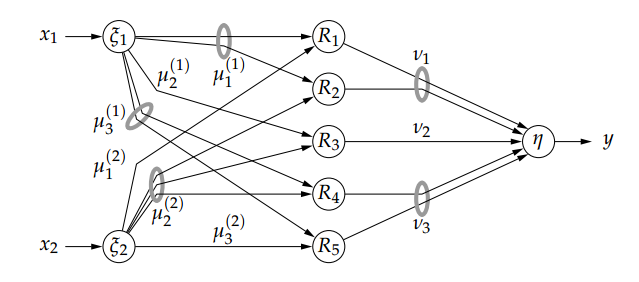
\includegraphics[scale=0.5]{images/nefcon_abb.png}
	\caption{NEFCON-Modell \cite{CIKruse:15}}\label{NEFCON_Abb}
\end{figure}

%\begin{align}

%\end{align}
% Hier Grafik einfügen

Das NEFCON-Modell basiert auf einem generischen Fuzzy-Perzeptron. Das Modell konnte in drei Schichten aufgeteilt werden. Die \textit{erste Schicht} besteht natürlich aus den Eingangsneuronen. Die ist eindeutig und will nicht weiter darauf eingehen. In der \textit{zweiten Schicht} befinden sich die inneren Neuronen, die die Regeln einer Fuzzy-System widerspiegeln. Im Beispiel sind insgesamt fünf Regeln gegeben. Die Fuzzy-Mengen $\mu_r^{(i)}$, die in Mehrere Regeln vorhanden sind, werden durch Ellipse zusammengeführt. Falls beim Lernen eine Anpassung an einem Gewicht durchgeführt werden soll, muss dies in allen Verbindungen gemacht werden, wo die Menge figuriert.

Der eigentliche Lernprozess besteht aus zwei Phasen. In der erste Phase wird versucht, eine Regelbasis erlernt zu werden. Diese Phase wurde weggelassen, falls schon eine existiert. Es lassen sich auch unvollständige sogar fehlende Regelbasen lernen. Für das Letztere ist ein weiterer Algorithmus erforderlich.

In der zweiten Phase findet die Optimierung statt. Dabei werden Fuzzy-Sets modifiziert oder selbst die Verbindungen zu den Regeln umgetauscht. In dem NEFCON-Modell wird als Bewertungsmaß, der ``Kritiker'', ein Fuzzy-Error verwendet. Damit die Optimierung optimal ausgeführt werden kann, sollte das Vorzeichen des Ausgabewertes bekannt sein. Darüber hinaus wird ein erweiterter Fuzzy-Error $E^*$ berechnet:
\begin{equation}\label{EFE}
E^* = sgn(y_{out})\cdot E(x_1, \ \ldots , \ x_n)
\end{equation}
\cite{CIKruse:15} \cite{UNIMAG:97}
\section{Erlernen einer Regelbasis}

Es existieren mehrere Algorithmen zum Erlernen von Regelbasis. Die Methoden können in drei Kategorien aufgeteilt werden: solche, die ohne vordefinierte Regelbasis startet; solche mit vollständiger Regelbasis und solche mit zufälliger Basis  starten. In den folgenden zwei Unterkapiteln werden Methode für die ersten zwei Kategorien vorgestellt. Bei den Methoden wird keine feste Lernaufgabe benötigt. Tatsächlich geht es darum, dass eine Initialbasis aufgebaut wird, ohne eine große Datenmenge mit optimalen Werten bekannt zu sein. \cite{CIKruse:15} \cite{UNIMAG:97}% Bis Hier drübergeguckt

\subsection{Top-Down- oder Reduktionsmethode zum Erlernen einer Regelbasis}

Zum Einen wird die Methode der Top-Down-Methode (in der Literatur auch als NEFCON I bekannt) genannt. Das Verfahren erfordt, dass eine vollständige Regelbasis vorhanden ist. Die Regelbasis beinhaltet auch widersprüchliche Regeln, die in Laufe des Prozesses ausgefiltert werden.

Der Prozess kann in zwei Phasen aufgeteilt werden. In der ersten Phase werden alle die Regeln eliminiert, die bei ihrer Ausgabe den falschen Vorzeichen aufweisen. Die auszufilternden Regeln werden mit der erweiterten Fuzzy-Fehler-Funktion (siehe \ref{EFE}) bestimmt. In der zweiten Phase werden Regeln mit identischer Prämisse zufällig ausgewählt. Folglich wird der Fehler für die bestimmte Regel berechnet. Zum Schluss wird die Regel ausgewählt, die die kleinste Fehlerrate aufweist. Die restlichen Regeln werden verworfen.

Eins der Nachteile der Top-Down-Methode ist die Aufwändigkeit, weil es mit einer großen Regelbasis gestartet wird. Das nächste Verfahren ist das Gegenteil von Top-Down-Methode, zwar Bottom-Up-Methode. \cite{CIKruse:15}


\subsection{Bottom-Up- oder Eliminationsmethode zum Erlernen einer Regelbasis}

Der Bottom-Up-Algorithmus beginnt mit einer leeren Regelbasis. Jedoch muss eine initiale Aufteilung(Intervall) der Ein- und Ausgabewerten gegeben sein. Analog zur Top-Down besteht diese Methode auch aus zwei Phasen. 

Erste Phase beginnt mit der Bestimmung der Prämisse für die Regeln. Der Prozess evaluiert jede Fuzzy-Menge mit bestimmten Eingaben und die Mengen, die den höchsten Zugehörigkeitsgrad aufweisen, werden ausgewählt. Aus den ausgewählten Fuzzy-Mengen werden neue Regeln gebaut. Danach versucht der Algorithmus eine geeignete Ausgabe aus dem aktuellen Fuzzy-Fehler zu ``raten''. Dabei wird vorausgesetzt, dass Eingaben mit ähnlichen Fehlerwerten ähnliche Ausgaben liefern.

In der zweiten Phase werden die Fuzzy-Mengen in den Konklusionen optimiert. Dabei werden nicht die Parametern der Konklusionen angepasst, sondern bei Bedarf die Fuzzy-Menge durch eine andere ersetzt.

Wegen des inkrementellen Lernen lässt sich einfach Vorwissen in dem Regelbasis einführen. Bei den Fällen mit unvollständigen Regelbasen werden passende Regeln hinzugefügt. Das Verfahren garantiert jedoch nicht, dass immer eine geeignete Regelbasis aufgebaut wird. Aus diesem Grund ist es empfohlen, dass die Regelbasis manuell am Ende des Lernens überprüft und entsprechend angepasst wird. \cite{CIKruse:15} \cite{UNIMAG:97}

\section{Optimierung der Regelbasis}

Die Optimierung bei NEFCON verwendet die Methode ``Back Propagtion Method'', oder Rückpropagationsmethode. Der Fehler wird rückwirkend durch das Netz geführt und lokal bei jeder Fuzzy-Menge angewendet.

Eine Änderung darf sowohl in den Prämissen, als auch in den Konklusionen. Es wird das Prinzip des verstärkenden Lernens angewendet. Das bedeutet, dass für jede Änderung eine Fuzzy-Menge entweder ``bestraft'' oder ``belohnt'' wird. Bestrafung und Belohnung werde in Änderungen wie Verschiebung, Vergrößerung oder Verkleinerung des Bereichs einer Fuzzy-Menge ausgedrückt. Änderungen werden entsprechend iterativ in Beziehung zum Fuzzy-Fehler gemacht. \cite{CIKruse:15} \cite{UNIMAG:97}

\section{Schlussworte}

% Zusammenfassung der zwei Methoden,
Die Methoden unterscheiden sich in ihrem Kern kaum. Beide Architekturen besitzen entsprechend Vorteile und Nachteile. Der größte Unterschied liegt in der Ausbau ihrer Struktur. ANFIS basiert auf TSK-Modellen, währen NEFCON auf die Mamdani-Reglern. Beide Modelle bieten sie sich gut für das Lernen von Fuzzy-Systeme, jedoch entspricht nur das ANFIS meinem Anwendungsfall - Optimierung von TSK-Modelle.
%% !TeX spellcheck = en_US
\chapter{Unscharfe Daten und Fuzzy-Logik}
In dem normallen Alltag eines Menschen werden ständig Aussagen über Ereignisse getroffen. Diese Aussagen können möglichst exakt sein, oder auch nicht. In manchen Situationen werden solche genannt, die für den Menschen adäquat ein Ereignis beschreiben. Man würde zum Beispiel sagen, dass es gerade sehr stark regnet, oder es sehr heiß ist. Diese Information kann von dem menschlichen Gehirn angemessen vearbeitet werden. Maschinen, wie Komputern, sind jedoch nicht mit dieser Funktionalität ausgestattet. Die sogenannten unscharfe Daten müssen somit anders repräsentiert werden, damit auch Maschinen diese verarbeiten können. Auf dieser Weise können wir den Vorteil der Maschinen gegenüber Menschen ausnutzen - ihre große Kapazität und die Möglichkeit komplexere Strukturen und Systeme darzustellen. In diesem Kapitel wird eine Erweiterung der klassischen Logik vorgestellt, die es den Komputern ermöglicht, unscharfe Daten darzustellen und darauf Operationen durchzuführen. Diese Logik ist als Fuzzy-Logik bekannt.

\section{Fuzzy-Logik}

%Eine Menge beschreibt ein Zusammenhang von Elementen, oder Objekte. Jedes Element erf�llt eine bestimmte Eigenschaften. In der klassischen Mengenlehre geh�rt ein Element entweder vollst�ndig oder nicht.

In der Literatur bezeichnet man die präzise Darstellung von unscharfen Daten als Fuzzy-Logic. Fuzzy-Logic unterscheidet sich von der klassischen Mengenlehre darin, dass Elemente graduell einer Menge gehören und nicht nur bivalente Zugehörigkeit erweisen können.

Zum Verdeutlichen betrachten wir die Menge M der reellen Zahlen, die viel größer sind als 1. 

\begin{align}
\centering
	M = \{ x \ |\ x \in \Re,\ x >> 1\}
\end{align}

Wird diese Menge mit der klassischen Logik modelliert, ergibt sich die Problematik: Der Vergleich ``viel größer'' ist mathematisch nicht eindeutig definiert. Auf die Grafik unten kann man die Modellierung mit der klassischen Logik sehen.

%Hier Graphik f�r die Set mit klassiche Darstellung viel gr��er als 1

\begin{figure}[htbp]
	\centering
	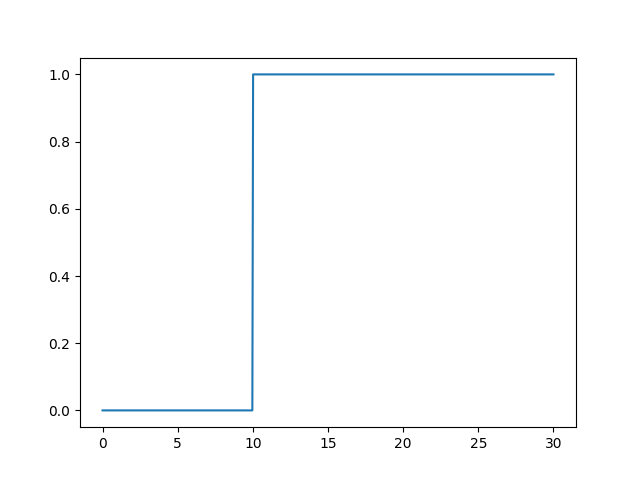
\includegraphics[scale=0.5]{images/classic_logic.png}
	\caption{``Viel größer als 1'' in der klassischen Logik}\label{class_dar}
\end{figure}

Aus der Graphik kann man feststellen, dass alle Werte kleiner als $10$ eine Zugehörigkeit von $0$ und solche größer oder gleich $10$ - eine Zugehörigkeit von $1$ besitzen. Diese Repräsentation entspricht jedoch die Realität nicht so ganz. Es ist eindeutig, dass ja $9.9$ als Wert schon größer als $1$ ist, aber der Graphik nach wird das nicht klar. Würde man diese Menge in der Fuzzy-Logik darstellen, ergibt sich folgendes Graph.

% Hier Graphik f�r die Fuzzy-Set "viel gr��er als 1"
\begin{figure}[htbp]
	\centering
	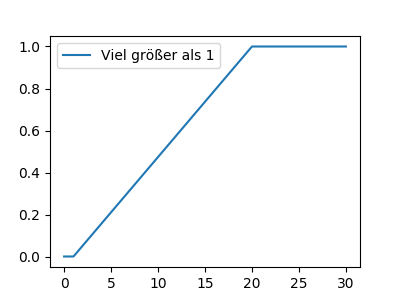
\includegraphics[scale=0.5]{images/fuzz_logic.png}
	\caption{``Viel größer als 1'' in der Fuzzy-Logik}\label{fuzzy_dar}
\end{figure}

Hier beschreibt die Graphik genauer, wie die Zahlen im Vergleich zu $1$ stehen. Die Zugehörigkeit nimmt Werte zwischen $0$ und $1$. Zum Beispiel der Wert $10$ hat die Zugehörigkeit von ca. $0.3$ und für Werte größer als $20$ liefert die Funktion $\mu (x)$ einen Wert von $1$ (volle Zugehörigkeit).


\subsection{Fuzzy-Sets}\label{fs_section}%Eventuell hier beschreiben
Fuzzy-Sets, oder Fuzzy-Mengen, beschreiben in der Fuzzy-Logik Eigenschaften von Elementen. Die Idee ist, dass Elemente zu einem rationallen Wert einer Menge gehören, beziehungsweise eine Eigenschaften besitzen. In der Literatur wird folgende Definition für Fuzzy-Mengen gegeben \cite{CIKruse:15}:

\begin{definition}
	Eine Fuzzy-Menge oder Fuzzy-Teilmenge $\mu$ der Grundmenge $X$ ist eine
	Abbildung $\mu : X \rightarrow [0, 1]$, die jedem Element $x \in X$ seinen Zugehorigkeitsgrad $\mu(x)$ zu
$\mu$ zuordnet. Die Menge aller Fuzzy-Mengen von $X$ bezeichnen wir mit $F(X)$. \cite{CIKruse:15}
\end{definition}

Normallen Mengen können als spezielle Fuzzy-Mengen aufgefasst werden. Also sind Fuzzy-Sets verallgemeinerte charakteristische Fuktionen \cite{CIKruse:15}.

In der Literatur tauchen unterschiedliche Arten von Fuzzy-Mengen. Die bekanntesten davon sind Dreiecksfunktion, Trapezfunktion und Gaußfunktion. Die Namensgebung kommt aus ihrer Form. Vier Beispielfunktionen sind unten gegeben.

\begin{figure}[htbp]
	\centering
	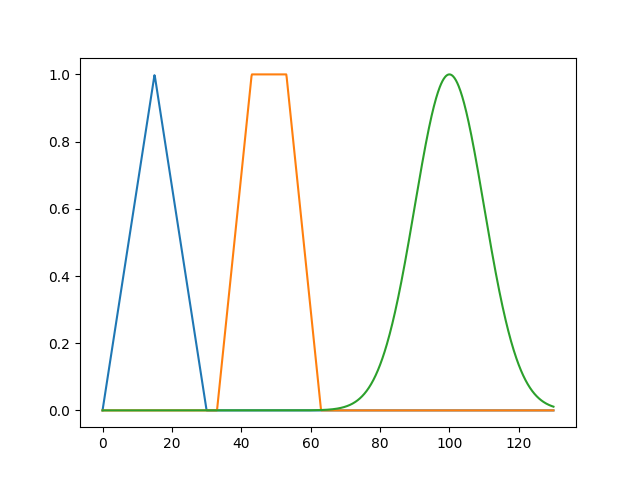
\includegraphics[scale=0.5]{images/mf_types.png}
	\caption{Arten von Fuzzy-Mengen}\label{mf_types}
\end{figure}

Die Form einer Fuzzy-Menge ist durch ihre Funktion bestimmt. Die Berechnung der Mengen wird folglich definiert.

\begin{equation}
	\mu_{tri}(x) = \begin{cases}
						\frac{x - a}{b - a} & \text{falls $a \leq x \leq b$}\\
						\frac{c - x}{c - b} & \text{falls $b \leq x \leq c$}\\
						0 & \text{sonst}
					\end{cases}
\end{equation}

Der Index der Funktion verdeutlicht, dass es sich um die Dreiecksfunktion handelt. Die Funktion hat drei Parametern, wo $a und c$ die Grenzenparametern sind und $b$ - der Gipfelpunkt. Außerdem muss $a < b < c$ gelten. Die Dreiecksfunktion ist ein besonderer Fall der Trapezfunktion, wo die Punkte, bzw. Parametern, der oberen Grudseite gleich sind. Deswegen ist die Gleichung \ref{trap_mf} für die Trapezfunktion sehr ähnlich \cite{CIKruse:15}.

\begin{equation}
\mu_{trap}(x) = \begin{cases}
\frac{x - a}{b - a} & \text{falls $a \leq x \leq b$}\\
1 & \text{falls $b \leq x \leq c$}\\
\frac{d - x}{d - c} & \text{falls $c \leq x \leq d$}\\
0 & \text{sonst}

\label{trap_mf}
\end{cases}
\end{equation}

Die Glockefunktion ist, wie ihrer Name andeutet, eine Funktion, die die Form einer Glocke hat. Die Darstellung dieser Funktion ähnelt sich sehr der Gaußsche Funktion. Die Berechnung wird untern gegeben. 

\begin{equation}
\mu_{bell}(x) = \frac{1}{1 + [(\frac{x - c}{a})^2]^b}
\label{bell_mf}
\end{equation}

Die letzte Funktion, die vorgestellt werden soll, ist die gaußsche Funktion. Die Formel wird öfters in der Statistik für Darstellung von Nominalverteilungen, aber auch in der Fuzzy-Logik. Die Gaußfunktion ist wie folgt definiert \cite{CIKruse:15}:

\begin{equation}
	\mu_{gauss}(x) = exp(\frac{-(x - m)^2}{s^2})
	\label{gauss_mf}
\end{equation}

Die Parametern $m und q$ sind entsprechend der Mittelwert (Mittelpunkt) und die Abweichung von der Mitte, oder als $\sigma$ (Sigma) in der Statistik bekannt.




%[Fuzzy-Logik und Fuzzy-Control, Jörg Kahlert; Hubert Frank,]
%
%
%   [Fuzzy-Logik und Fuzzy-Control, Jörg Kahlert; Hubert Frank, Computational Intelligence]

\section{Operationen auf Fuzzy-Sets}
In den vorherigen Kapiteln wurde auf die Wichtigkeit von Fuzzy-Logik, genau so wie Repräsentation von Fuzzy-Mengen eingegangen. Um nun unscharfe Informationen verarbeiten zu können, wie Schlüsse daraus zu ziehen oder mehrere Fuzzy-Mengen zu kombinieren, brauchen wir eine Reihe von Operatoren. Da es um Mengen geht, eignen sich die Durchschnitt-, Vereinigung- und Komplementbildung aus der klassischen Logik gut. Im folgenden Kapitel werden die einzelnen Operationen beschrieben [Computational Intelligence].

\subsection{Durchscnitt}\label{AND}

In der klassische Logik ist der Durchschnitt durch einen Logischen-UND eingesetzt. In der klassischen Mengenlehre ist die Menge aller Elementen, die zu einer Menge $M_1$ und einer Menge $M_2$ gehören, als Schnittmenge definiert. Gegeben seien die Mengen:

\begin{align}
M_1 = \{ x \ | \ x \in\Re, \ 1 \ \leq \ x \ \leq \ 3 \} 
\end{align}
\begin{align}
 M_2 = \{ x \ | \ x \in\Re, \ 2 \ \leq \ x \ \leq \ 4 \} 
\end{align}

Der Durchschnitt der beiden Mengen ergibt sich:

\begin{align}
M_1 \cap M_2 = \{ x \ | \ x \in \Re, \ 2 \ \leq \ x \ \leq \ 3 \}
\end{align} 

Der UND-Operator lässt sich analog auf die Fuzzy-Mengen anwenden. Es wird die Fläche bestimmt, die für beide Mengen erfüllt ist. Aus methematischer Sicht sprechen wir von dem Minimum-Operator(MIN).

%\theoremstyle{definition}
\begin{definition}
	Seien $\mu_1$ und $\mu_2$ zwei Fuzzy-Mengen auf der Grundmenge $G$. Dann heißt:
		\begin{center}
			$\mu_1$ $\cap$ $\mu_2$ : $G$ $\rightarrow$ [0,1] $\text{mit}$ ($\mu_1$ $\cap$ $\mu_2$)($x$) $=$ MIN($\mu_1$($x$) , $\mu_2$($x$)) 
		\end{center}
	der \textbf{Durchschnitt} der Fuzzy-Mengen $\mu_1$ und $\mu_2$.
\end{definition} 

Zur Veranschaulichung wird unten die Grafik angegeben. Da sind zwei Fuzzy-Sets dargestellt. Die zwei Ausdrücke, die betrachtet werden, sind $mittlere$ und $hohe$ Temperatur. Der rote gestrichene Bereich stellt die Ergebnismenge dar.

\begin{figure}[htbp]
	\centering
	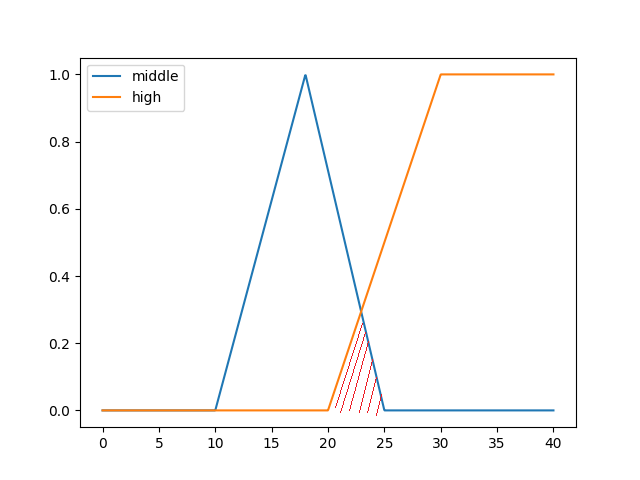
\includegraphics[scale=0.5]{images/und_high_middle_temp.png}
	\caption{Durchschnitt von zwei Fuzzy-Mengen (blauer gestrichener Bereich)}\label{high_low_temp_intersection}
\end{figure}

%hier Grafik f�r die Mittlere und Hohe Temperatur mengen.


\subsection{Vereinigung}

Nehmen wir ganz einfach die Definition der Vereinigung aus der klassischen Mengenlehre:
	\begin{center}
	$x$  $\in$ $M_1$ $\cup$ $M_2$ $\Leftrightarrow$ $x$ $\in$ $M_1$ $\vee$ $x$ $\in$ $M_2$
	\end{center}

Ziemlich eindeutig und klar. Die Vereinigungsmenge enthält alle diese Elemente aus dem Grundbereich, die entweder in der Menge $M_1$ oder $M_2$ enthalten sind. Im nächsten Schritt wird dieser Operator an die Fuzzy-Mengen angepasst.

In der Mathematik ist dieser Operator als ODER-Verknüpfung angegeben. Die Anwendung der ODER-Operator auf Fuzzy-Mengen wird wie folgt dann definiert:

%\theoremstyle{definition}

\begin{definition}
	Seien $\mu_1$ und $\mu_2$ zwei Fuzzy-Mengen auf der Grundmenge $G$. Dann heißt:
	\begin{center}
		$\mu_1$ $\cup$ $\mu_2$ : $G$ $\rightarrow$ [0,1] $\text{mit}$  ($\mu_1$ $\cap$ $\mu_2$)($x$) $=$ $MIN$($\mu_1$($x$)), $\mu_2$($x$)) 
	\end{center}
	die $\textbf{Vereinigung}$ der Fuzzy-Mengen $\mu_1$ und $\mu_2$.
\end{definition}

Betrachten wir den selben Beispiel aus vorherigen Unterkapitel. Seien also wieder die Fuzzy-Mengen für \textit{``mittlere''} und \textit{``hohe''} Temperatur. Wenn wir den ODER-Operator auf die beiden Mengen anwenden, ergibt sich eine Ergebnismenge, die sich auf beiden Mengenflächen aufstellt. Dies wurde graphisch zunächst aufgezeichnet.

\begin{figure}[htbp]
	\centering
	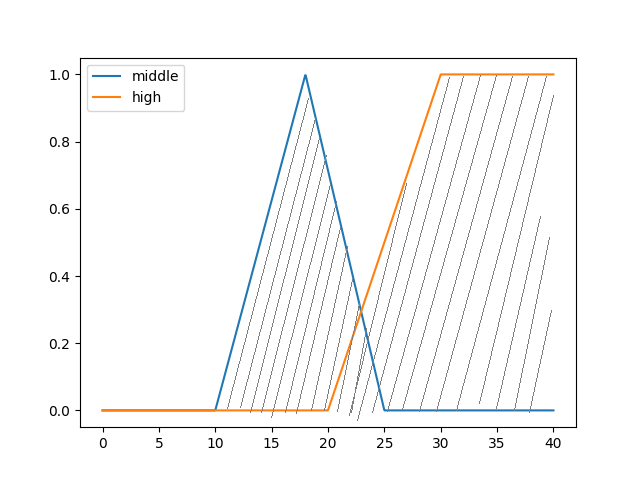
\includegraphics[scale=0.5]{images/oder_mid_high_temp.png}
	\caption{Union von Fuzzy-Mengen (gestrichener mit Rot Bereich)}
\end{figure}\label{high_low_temp_union}
% Hier Graphik f�r Oder verkn�pfung  

\subsection{Komplement}

Der dritte wichtige Operator ist das Komplement einer Menge. In der klassischen Mengenlehre ist dieser Operation ziemlich einfach anzuwenden. Der Operator beschreibt die Negation einer Aussage - zum Beispiel die Wahrscheinlichkeit eine 6 zu würfeln wäre $\frac{1}{6}$, die Gegenwahrscheinlichkeit, oder die Wahrscheinlichkeit etwas anderes als 6 zu würfeln wäre: (1 - $\frac{1}{6}$) = $\frac{5}{6}$. Das Komplement ist in der Fuzzy-Logik dann wie folgt definiert: 

\begin{definition}
	Sei $\mu$ eine Fuzzy-Menge auf der Grundmenge $G$. Dann heißt:
	\begin{center}
		$\mu^c$  : $G$ $\rightarrow$ [0,1] $\text{mit}$  ($\mu^c$)($x$) $=$ $1$ - $\mu$($x$)) 
	\end{center}
	die $\textbf{Vereinigung}$ der Fuzzy-Mengen $\mu_1$ und $\mu_2$.
\end{definition}

Zur Veranschaulichung die Menge \textit{hohe} Temperatur negiert. Die Negierung ist in der Graphik unten zu sehen.

%Hier Grafik f�r das Komplement-Beispiel

\begin{figure}[htbp]\label{not_high_temp}
	\centering
	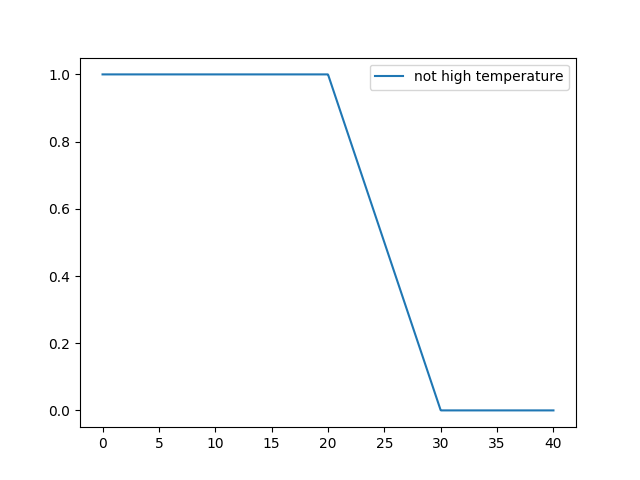
\includegraphics[scale=0.5]{images/not_high_temp.png}
	\caption{Komplement der Menge hohe Temperatur}
\end{figure}

\subsection{Zusammenfassung}

In diesem Kapitel habe ich die drei wichtigsten Operatoren auf Fuzzy-Mengen vorgestellt. Neben den Grundverknüpfungen gibt es eine weitere Sammlung von Verknüpfungsoperatoren.

\begin{enumerate}
	\item Algebraisches Produkt: ($\mu_1$$\mu_2$) = $\mu_1$($x$) $\cdot$ $\mu_2$($x$)
	\item direkte Summe: ($\mu_1$ $\bigoplus$ $\mu_2$) = $\mu_1$($x$) + $\mu_2$(x) - $\mu_1$($x$) $\cdot$ $\mu_2$($x$)
	\item abgeschnittene Differenz: ($\mu_1$ $\sqfrowneq$ $\mu_2$) = MAX(0, $\mu_1$(x) + $\mu_2$(x) - 1)
	\item abgeschnittene Summe: ($\mu_1$ \^{+} $\mu_2$) = MIN(1, $\mu_1$(x) + $\mu_2$(x))
	\item ($\mu_1$$\dotminus$ $\mu_2$) = MIN($\mu_1$(x), 1 - $\mu_2$(x))
	\item ...
\end{enumerate}

Dies ist eine Vorbereitung auf die folgenden Kapiteln. Wir analysieren mehrere Fuzzy-Mengen und ziehen daraus bestimmte Schlüsse. Ein Beispiel dafür wäre: Wenn eine Tomate rot ist, dann ist die reif. Folgende Logische Aussagen können sehr einfach mit Fuzzy-Logic modelliert werden. In der Literatur taucht die Name Fuzzy-Regeln. Diese können dann zusammengestellt werden, um Fuzzy-Regel-Systeme aufzubauen. Die nächste Kapitel stellt Fuzzy-Systeme vor. 

\section{Fuzzy-Systeme}

Ein Fuzzy-System, auch Fuzzy-Regler oder Fuzzy-Inferenz-System, ist ein bekannter Framework basierend auf Fuzzy-Mengen-Theorie, Fuzzy Wenn-Dann-Regeln und Fuzzy Reasoning. Konzeptionell besteht ein Fuzzy-System aus drei Grundteile - die Regelbasis, welche die Wenn-Dann-Regeln beinhaltet; die Datenbank(oder das Wörterbuch), die alle Zugehörigkeitsfunktionen definiert; und der Entscheidungmechanismus, wer die Inferenz durchführt und eine angemessene Schlussfolgerung erkundet.   

Folglich werden zwei Arten von Fuzzy-Systeme erläutert.

\subsection{Mamdani-Regler}

Der Mamdani-Regler wurde im Jahr 1975 von Mamdani auf der Basis einer Veröffentlichung von Zadeh aus der Anfang der siebziger Jahren entwickelt. 

Der Mamdani-Regler ist eine endliche Menge von Wenn-Dann-Regeln $R$ der Form:
\begin{equation}
	R: \text{If } x_1 \text{ is } A_1 \text{ and ... and } x_n \text{ is } A_n
	\text{ then } y^\prime \text{ is } B
\end{equation}

In der Regel sind $x_1$, ..., $x_n$ die Eingangsgrößen und $y^\prime$ die Ausgabe. $A_i$ und $B$ sind  linguistischen Werte. Jede Regel besteht aus zwei Teilen - Prämissen und Konklusionen. Jede Vorbedingung untersucht spezifische Eigenschaften. Es wird geprüft, ob der Eingangwert diese Eigenschaften erfüllt. Anhand diese Merkmale schließt sich eine Konklusion. 

Sei $W$ die Menge aller linguistischen Konklusionen $B_i$, so dass $B_1, \dots, B_m \in W$ gilt. Der Regler kann als eine n-Stellige Funktion mit $f: \mathbb{G^n} \mapsto W$ dargestellt werden. Die Funktion ordnet eine Eingabe zu einem linguistischen Term $B_i$.

\begin{equation}
	f(x_1, ..., x_n) \approx 
	\left\{
		\begin{array}{ll}
			B_1 & \mbox{ falls } x_1 \mbox{ is } A_1^{(1)} \mbox{ und ..., und } x_{n} \mbox{ is } A_n^{(1)}\\
			\vdots \\
			B_{m} & \mbox{ falls } x_1 \mbox{ is } A_1^{(m)} \mbox{ und ... und } x_{n} \mbox{ is } A_n^{(m)}
		\end{array}
	\right.
\end{equation}

In der Funktion gibt es genau so viele Ausgaben, wie es Regeln gibt - $m$.

Mit einem Mamdani-Regler können viele Probleme aus der reellen Welt definiert werden. Als kleines Beispiel eignet sich die Farben der Tomaten. Wir betrachten die Farbe als Eingabe. Die Ausgabe würde uns sagen, wie reif eine Tomate ist. Wir teilen unsere Eingangsgrößen in drei Farben: rot, gelb und grün. Daraus lassen sich entsprechend 3 Fuzzy-Mengen definieren. Als Ausgabe wird die Reife einer Tomate bestimmt. Das Ergebnis kann in drei Mengen anfallen: reif, halbreif oder unreif. Auf dieser Weise haben wir ein Mamdani-Fuzzy-Model, das aus 3 Fuzzy-Sets und aus 3 Regeln besteht. Die Regelbasis sieht wie folgt aus:

\begin{itemize}
	\item $R_1$: if x is rot, then y is reif.
	\item $R_2$: if x is gelb, then y is halbreif.
	\item $R_3$: if x is grün, then y is unreif.
\end{itemize}

Eine Tabelle für die Fuzzy-Relationen ist unten gegeben

\begin{table}\label{tomato:1}
	\centering
	\begin{tabular}{c|c c c}
		
		x \diagdown \ y & \ unreif & \ halbreif & \ reif \\ [0.5ex]
		\hline
		grün & 1 & 0 & 0 \\ 
		gelb & 0 & 1 & 0\\
		rot  & 0 & 0 & 1\\
		
	\end{tabular}
\caption{Beispiel für Tomaten}

\end{table}

Wie man sieht die Tabelle ist ziemlich einfach zu lesen, wenn die Tomate grün ist, wird immer angenommen dass sie unreif ist. Man könnte entsprechend die Fuzzy-Mengen aus der Konklusion verfeinern. Das würde bedeuten, dass die Mengen sich überlappen. Unsere Tabelle könnte dann wie folgt aussehen:

\begin{table}
	\centering
	\begin{tabular}{c|c c c}
		
		x \diagdown \ y & \ unreif & \ halbreif & \ reif \\ [0.5ex]
		\hline
		grün & 1 & 0.5 & 0 \\ 
		gelb & 0.3 & 1 & 0.3\\
		rot  & 0 & 0.5 & 1\\
		
	\end{tabular}
	\caption{Beispiel für Tomaten}
	\label{table:1}
\end{table}

Abhängig davon wie man die Ausgangsmengen definiert, wie weit die Mengen überlappen, ergibt sich eine unterschiedliche Interpretation der Werte. Je mehr Fuzzy-Sets für eine Größe(Maß) definiert sind, desto besser könnte ihr Zustand repräsentiert werden. Mit der Anzahl der Fuzzy-Sets steigt die Komplexität eines Systems proportional.

Den oberen kleinen Beispiel zeigt wie einfach Mamdani-Modelle zu modellieren sind. Mamdani-Reglern finden in der Praxis öfters Einsetzung.

\subsection{Takagi-Sugeno-Kang-Modell} \label{TSK}

Das Takagi-Sugeno-Kang-Modell ist dem Mamdani-Modell sehr ähnlich. TSK-Regler verwenden Regeln der Form:

\begin{align}
	R: \text{ If } x_1 \text{ is } \mu_R^{(1)} \text{ and \ldots and } x_n \text{ is } \mu_R^{(n)} \text{ then } y = f_R(x_1,\ldots,x_n).
\end{align}}

In den Prämissen ist kein Unterschied zu erkennen. Die Besonderheit des TSK-Modells liegt in der Konklusion. Da steht eine linear Funktion, anstatt eine Fuzzy-Menge. In der Konklusion kann im Allgemeinfall jede beliebige Funktion $f$ in der Eingabe von $x$ berechnet werden. Normalerweise ist $f$ eine linear Funktion, die wie folgt aussieht:
\begin{align}
	f(x_1, \ldots, x_n) = p_0 + p_1\cdot x_1 + \ldots + p_n\cdot x_n,
\end{align}
$p_0, \ldots, p_n$ sind die Parametern der Konklusionsfunktion. Für geiegnete ausgewählte Parameterwerte modelliert das TSK-Modell eine mathematische Funktion, dies kann z.B. die Quadratfunktion sein. Für den Fall, dass die Parametern $p_1, \ldots w_n$ den Wert 0 haben, erhält man einen Mamdani-Modell mit scharfer Ausgabe. Solche Modelle heißen in der Literatur auch \textbf{zero-order Sugeno-Fuzzy-Modelle} \cite{SCTemassi:01, NFMBothe:98, NFSC:97}.
Als Beispiel kann folgende Regelbasis betrachtet werden:
\begin{align}
R_1: \text{ If } x \text{ is ``sehr klein'' then } y = 0\\
R_2: \text{ If } x \text{ is ``klein'' then } y = 1\\
R_3: \text{ If } x \text{ is ``groß'' then } y = 2\\
R_4: \text{ If } x \text{ is ``sehr groß'' then } y = 3.
\end{align}
Die Fuzzy-Sets sind ``sehr klein'', ``klein'', ``groß'' und ``sehr groß'' und die Ergebnisswerte entsprechend \textit{0, 1, 2 und 3}.

\subsection{Fuzzifizierung und Defuzzifizierung}\label{FDF} 

Der Vorgang eines Modells zerlegt sich in zwei Teilen - Fuzzifizierung und Defuzzifizierung. Der erste Begriff beschreibt den Prozess für die Evaluierung der Eingangswerte in Fuzzyinferenzsysteme. Es gibt mehrere Evaluierungsmethoden, beziehungsweise Fuzzifizierungsmechanismen, wie zum Beispiel die Gaußsche Funktion (\ref{fs_section}). Der zweite Begriff bezeichnet die Vorgehensweise bei der Berechnung der Ausgabe, oder Inferenz, eines Fuzzy-Systems. Die Reihenfolge der beiden Prozesse ist somit bestimmt. Da im vorrigen Kapitel schon Beispiele für Fuzzifizierungsverfahren vorgestellt werden, steige ich demnächst in den unterschiedlichen Arten von Defuzzifizierung.

Bei der Regelaktivierung unterscheidet man zwei Fällen. Wenn die Eingabe einer volle Zugehörigkeit ergibt, dann liefert das Modell ganz normal den Wert der entsprechenden Konklusionsfunktion. Bei partielle Aktivierung mehreren Regeln ergibt sich das Inferenzergebnis aus einem spezifischen Verfahren. Dafür werden bestimmte Inferenzmethoden angewendet, zum Beispiel das Center of Gravity, oder Center of Area. Einige dieser Methoden werden inden folgenden Unterkapiteln vorgestellt. In allen Verfahren handelt es sich, um Mamdani-Reglern, wo die Konklusion einer Regel aus einer Fuzzy-Mengen besteht. Die letzte vorgestellte Methode ist spezifisch für Takagi-Sugeno-Kang-Modelle anzuwenden.

\subsubsection{Height Method}
Bei dieser Methode, auch als \textit{maximum membership principle} bekannt, wird der Regelaktievierung mit den größten Wert ausgewählt. Die Vorgehensweise könnte in Systeme verwendet werden, wo der größte Zutreffer nur wichtig ist. Als Beispiel könnte ein System mit entsprechenden Gegenmaßnahmen genannt werden, wo der größte Risiko Vorgang haben soll \cite{SCTemassi:01}.

\subsubsection{Center of Gravity}

Center of Gravity, auch als Center of Area bekannt, ist die prominenteste Methode von allen, wo sich das Ergebniss als schärfer Wert ergibt. Das Endergebniss berechnet sich aus folgender Formel:
\begin{align}
	y^* = \frac{\int y \cdot \mu_R(y)dy}{\int \mu_R(y)dy}
\end{align}

Der Wert \textit{y} hier ist das Ergebnis der aktivierte Regel \textit{R} und \textit{$y^*$} ist das Endergebniss. \cite{SCTemassi:01}

\subsubsection{Weighted Average Method}

Die gewichtete Durchschnittsmethode, oder Weighted Average Method, ist nur für Ausgangszugehörigkeitsfunktionen, die aus mehreren symmetrischen Zugehörigkeitsfunktionen $\mu_i$ besteht. Die Formel lautet:
\begin{align}
y^* = \frac{\sum_{i} \=y \cdot \mu_i(\=y)}{\sum \mu_i(\=y)}
\end{align}

Das Modus jeder Zugehörigkeitsfunktion $\mu_i$ wird duch den Wert von $\=y$ beschrieben. \cite{SCTemassi:01}

\subsubsection{Takagi-Sugeno-Kang-Defuzzifizierungsmethode}
Die Defuzzifizierungsmethode von TSK-Modelle berechnet eine Interpolation zwischen den Ausgangswerte. Die Formel nimmt den Ausgabewert jeder Regel und multipliziert den mit dem Gewicht, der Regelaktievierung, der entsprechenden Regel und gewichtet durch die Wahrheitsrate jeder Regel. Die Formel ist gegeben:
\begin{align}\label{TSK_defuzz}
y = \frac{\sum_{i} \mu_i \cdot f_i(x_1, ..., x_n)}{\sum \mu_i},
\end{align} wo $\mu_i$ die Wahrheitsrate, bzw. Aktievierungswert, einer Regel $i$ ist und $f_i$ liefert den Ergebniswert für die Regel bei Eingabe $x_1, ..., x_n$.

Zum Schluss wird eine Abbildung gegeben, die den gesammten Prozess, Fuzzifizierung und Defuzzifizierung, darstellt. Die Abbildung beschreibt, wie das Endergebnis berechnet wird.

\begin{figure}[htbp]
	\centering
	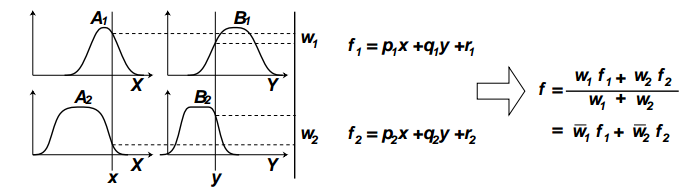
\includegraphics[scale=0.5]{images/TSK_Modell.png}
	\caption{Inferenzschritt eines TSK-Modells \cite{Jang:93}}\label{TSK_Modell}
\end{figure}

In der Figur wird ein Model mit zwei Eingangsgrößen und zwei Fuzzy-Mengen pro Eingabe dargestellt. Die Regelbasis besteht aus zwei Regeln und sind in der Reihe zu lesen. Die Fuzzy-Mengen werden durch die Glockefunktion berechnet. Die Variablen $w_1$ und $w_2$ liefern die Regelaktievierungen für die Regeln mit entsprechenden Indexen. Das Endergebnis $f$ ergibt sich aus der oben definierte Funktion \ref{TSK_defuzz}, wobei $w_1$ und $w_2$ der Variablen $\mu_1$ $\mu_2$ entsprechen.

%Unsicher ob ich darauf eingehen soll

%Die Gliederung h�ngt nat�rlich vom Thema und von der L�sungsstrategie ab. Als n�tzliche
%Anhaltspunkte k�nnen die Entwicklungsstufen oder - schritte z.B. der Softwareentwicklung betrachtet werden. N�tzliche Gesichtspunkte erh�lt und erkennt man, wenn man sich
%\begin{itemize}
%  \item in die Rolle des Lesers oder
%  \item in die Rolle des Entwicklers, der die Arbeit z.B. fortsetzen, erg�nzen oder pflegen soll,
%\end{itemize}
%versetzt. In der Regel wird vorausgesetzt, dass die Leser einen fachlichen Hintergrund haben - z.B. Informatik studiert haben. D.h. nur in besonderen, abgesprochenen F�llen schreibt man in popul�rer Sprache, so dass auch Nicht-Fachleute die Ausarbeitung prinzipiell lesen und verstehen k�nnen.
%
%Die �u�ere Gestaltung der Ausarbeitung hinsichtlich Abschnittformate, Abbildungen, mathematische Formeln usw. wird in \hyperref[Stile]{Kapitel~\ref*{Stile}} kurz dargestellt.
%\chapter{Künstliche Neuronale Netze} \label{ANN}

Künstliche Neuronale Netze (engl. artificial neural networks) sind Systeme, die auf dem Gehirn von Tieren und Menschen basieren und besteht aus endlich viele Einheiten, Neuronen. Der Datenaustausch geschieht über gerichtete Verbindungen zwischen den Neuronen. Forscher beschäftigen sich mit Neuronalen Netzen aus unterschiedlichen Gründen. In der Biologie simulieren Forscher diese, um sich den Prozess des Lernens und weitere Mechaniscmen zu untersuchen. In der Informatik wird aber versucht, die Lernfähigkeit des Gehirns nachzubilden und auszunutzen.

In den folgenden Kapiteln wird zuerst auf den Neuronen sowohl in der Biologie als auch in der Künstliche Intelligen eingegangen. Weiterhin werden die Eigenschaften von Neuronalen Netzen erklärt. Zum Schluss stelle ich den Gradientenvarfahren vor, anhand dessen diese Netze lernen.

\section{Biologische Grundlagen}

Das tierische Gehirn leitet jede einzelne Aktivität in dem Körper eines Tieres, inklusive die Verarbeitung von Daten. Laut \cite{GEHIRN:12} besteht das Gehirn aus 86 Milliarden Neuronen, die in Cliquen verbunden sind. Neuronen in einer Clique komunizieren untereinander, indem sie Signale über ihre Axone weiterleiten und Signale über ihren Dendrit empfangen. Eine Verbindung zwischen Neuronen existiert, wenn die Axonterminale eines Neurons den Dendrit eines anderen berührt. Zur Veranschaulichung ist den Aufbau eines Neurons in Abbildung \ref{neuron} gegeben. Jeder Signal wird in dem Soma verarbeitet und durch die Axone weitergeschickt.

\begin{figure}[!htbp]
	\centering
	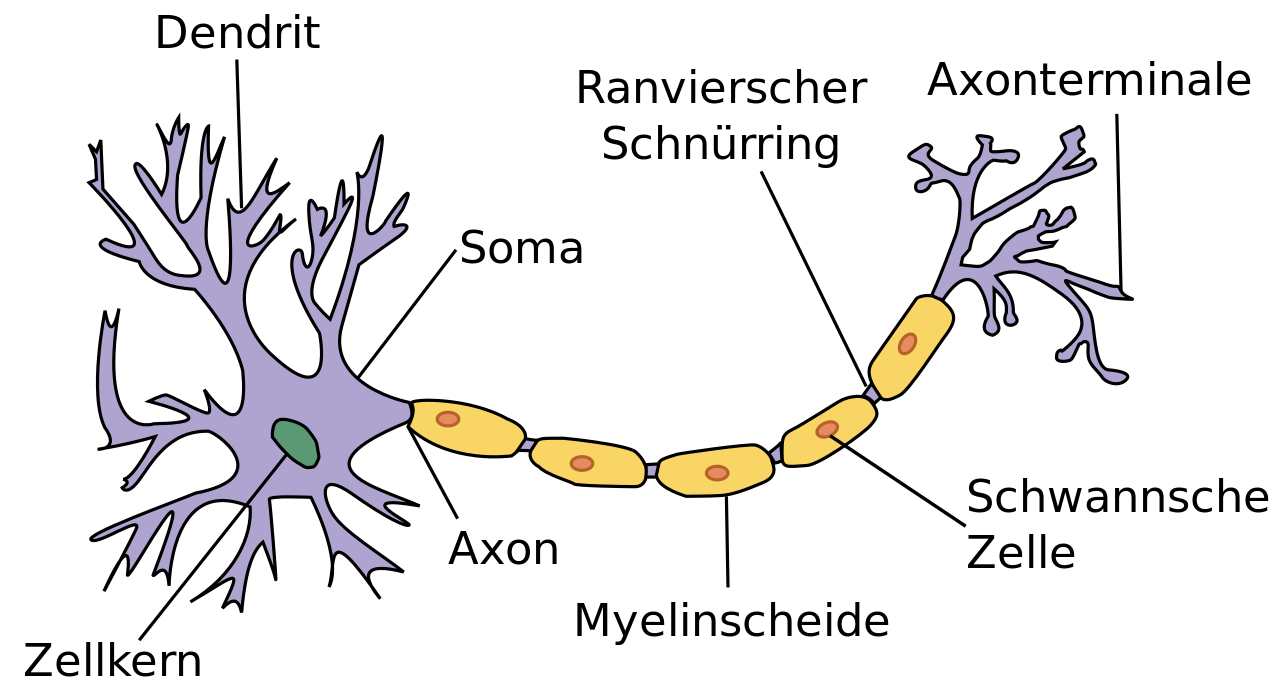
\includegraphics[scale=0.2]{images/Neuron_(deutsch)-1.png}
	\caption{Neuron \cite{NWIKI:19}}\label{neuron}
\end{figure}

Auf dem selben Prinzip funktionieren auch Neuronen in Künstlichen Neuronalen Netzen (KNN). Im folgenden Kapitel wird mehr darauf eingegangen. \cite{NWIKI:19} \cite{GEHIRN:12}

\section{Neuron in Künstlichen Neuronalen Netzen}

Neuronale Netze sind streng genommen gerichtete Graphen, wo jeder Knoten ein Neuron ist und jede Kante eine Verbindung zwischen Neuronen beschreibt. Die Neuronen können in drei Gruppen, oder auch als Schichten (\textit{engl.} Layers) bekannt, unterteilt werden - Eingabe-, Ausgabe- und versteckte Neuronen. Die Ein- und Ausgabeknoten sind die Einheiten, die mit der Umgebung verbunden sind, dabei ist klar welche Knoten was sind. Die übrigen Elemente werden in dem Netz eingebaut und kommunizieren nur mit anderen Neuronen. Daraus ergibt sich auch ihren Namen ``versteckt''.

Jede Verbindung zwischen Neuronen in KNN erhält ein Wert. Der Verbindungswert wird meistens als Gewicht bekannt. Bei einem Gewicht von 0 existiert keine Verbindung zwischen Neuronen. In einem KNN werden nur die Gewichte gelernt, während die Neuronen nur eine mathematische Funktion beschreiben. Eine übliche Repräsentation der Gewichte ist eine Matrix \ref{knnmat}.

\begin{align}
	\label{knnmat}
	\bordermatrix{ 	
			   & u_1 			& u_2			 & \dots & u_r			    \cr
		u_1    & w_{u_{1}u_{1}} & w_{u_{1}u_{2}} & \dots & w_{u_{1}u_r}		\cr
		u_2	   & w_{u_{2}u_{1}} & w_{u_{2}u_{1}} & 	     & w_{u_{2}u_{1}}	\cr
		\vdots & \vdots	      	& 			     &       & \vdots			\cr
		u_r    & w_{u_{r}u_{1}} & w_{u_{r}u_{2}} & \dots & w_{u_{r}u_r}  	\cr 
	}
\end{align}

Die Beziehungen zwischen Neuronen aus zwei Schichten wird außerdem ganz gut in der Matrix dargestellt. Sie ist von oben nach rechts zu lesen, also die Spalten sind es dem Neuronen zugeordnet, aus denen die Verbindungen ausgehen. Das heißt der Knoten $u_1$ hat eine Verbindung zu sich selbst und dem Neuron $u_2$ und die Gewichtwerte sind entsprechend $w_{u_{1}u_{1}}$ und $w_{u_{1}u_{2}}$. Die Darstellung als Matrix erlaubt es alle mathematischen Operationen durchzuführen, indem der Ausgabe eines Neurons, oder die Eingabe aus der Umgebung, rechts an der Matrix dranmultipliziert. \cite{CIKruse:15} \cite{NFMBothe:98} \cite{SCTemassi:01} \cite{CISCNFI:98}

\section{Lernen} % s. 58 Book 2; s.40 Computational Intelligence s. 21
Die erstaunlichste Eigenschaft Neuronaler Netze ist ihre Möglichkeit, eine Aufgabe, bzw. Fähigkeit, zu erlernen. Gewichtswerte und/oder weitere Parameter unterliegt Änderungen nach jeder Iterationsschritt während des Lernprozesses. In Bezug auf dem Iterationsschritt wird es zwischen ``Offline-'' und ``Onlinelernen'' unterschieden. Außerdem unterscheidet man zwei weiteren Gruppen in der Lernmethode eines Neuronalen Netzes - überwachtes (\textit{engl.} supervised) und unüberwachtes (\textit{engl.} unsupervised) Lernen. Demnächst werden die Begriffe einzeln untersucht. Danach werden nur beaufsichtigte Algorithmen vorgestellt, da die relevant für mein Projekt sind. Zum Schluss werden die Offline- und Online-Lernverfahren vorgestellt, die insgesammt drei sind.  \cite{SCTemassi:01} \cite{CIKruse:15} \cite{NFSC:97} %Nach jedem Schritt können Gewichtswerte und/oder weitere Parameter optimiert werden.

\subsection{Unsupervised Learning}
Unsupervised Learning (\textit{deutsch} unbeaufsichtigtes Lernen) besteht immer noch eine Ein-/Ausgabe beziehung, jedoch wird kein Fehlerfunktion eingesetzt. In diesem Fall muss das Netz Mustern aus den Ein-/Ausgabepaare erkennen und zusammengruppieren.

\subsection{Supervised Learning}

Unter Supervised Learning versteht man den Verfahren, bei dem das Netz anahand von Ein-/Ausgabepaare trainiert wird. Das Lernenprozess beinhaltet die allmäliche Anpassung der Gewichtparametern bei jedem Iterationsschritt, so dass bei gegebener Eingabe $x$ der Fehler, der aus der Ausgabe und dem Erwartungswert berechnet wird, minimiert wird. Die Fehlerfunktion wird in vielen Fällen auch als ``Kritiker'' und das Modell als ``Kritisierender'' bekannt. Ein Speziallfall des überwachtes Lernen ist ``reinforcement Learning''. In dem Lernverfahren wird jede Berechnung ``richtig'' oder ``falsch'' bewertet, ohne dass ein Fehler unbedingt berechnet wird. \cite{SCTemassi:01} \cite{CIKruse:15} \cite{NFSC:97}

\subsubsection{Least Mean Square Method}
Die Kleinste Quadrate Methode (\textit{engl.} Least Mean Square Method) wurde von den B. Widrow und M.Hoff für ein Projekt namens ADALINE oder ADAptive LINear Element entwickelt. Die Methode versucht die Fehlerrate mit dem Gradientenverfahren zu verringern. Die Fehlerrate wird mit dem Mean Squared Error (MSE) geteilt durch die Anzahl der Elementen im Trainingsdaten berechnet. Die Formel ist gegeben:

\begin{align}
	E(w) = \frac{1}{2} \sum_{i=1}^{m}(d_i - y_i)^2 \label{MSE}, 
\end{align}

wobei $w$ ist der Gewichtsvektor, und $d_i$ und $y_i$ entsprechend - Erwartungs- und Ausgabewert. Die Ableitung der Funktion ergibt den nächsten Iterationsschritt:

\begin{align}
	w^{t+1} = w^t + \mu(d_k^t - y_k^t)x_k^t.
\end{align}

Die Konstante $\mu$ kontrolliert die Konvergenz und Stabilität, \textbf{w} und textbf{x} sind Gewichtsvektor und Eingabe. Der Schritt wird durch den Exponent $t$ bestimmt - $t+1$ ist der nächste Schritt. Solange die Konstante entsprechend gewählt wird, konvergiert der Verfahren und der gesuchte Gewichtvektor kann gelernt werden. \cite{SCTemassi:01}

\subsubsection{Backpropagation Algorithm}
Der Backpropagation Algorithmus, oder auch als Gradient Descent bekannt, wurde laut \cite{SCTemassi:01} am Ende der 70er Jahren von Paul J. Warbos entwickelt. Dieses Verfahren hat die Interesse an Neuronalen Netzen wiederbelebt.

Der Algorithmus ist der bekannteste Lernalgorithmus für beaufsichtigtes Lernen. In dem Verfahren stecken zwei wichtige Konzepte. Zum einen liegt der Feedforwardphase vor, die dann folgendes Verhalten beschreibt: die Eingabe-/Erwartungswerte dem Neuronalen Netz gegeben werden und anschließend eine Ausgabe berechnet wird. Danach wird der Fehler berechnet, für den eine bestimmte Fehlerfunktion verwendet wird, z.B. der Mean Squared Error (siehe Gleichung \ref{MSE}). In der zweiten Phase, auch Rückwertsphase genannt, werden die Knoten rückwerts anfangend von der Ausgabe- über die versteckten Schichten bis zum Eingabeschicht angepasst. Das Ziel der Rückwertsschritt ist es den Fehlre zu minimieren. Hinter dem Verfahren stecken einfache Mathematische Operationen, wurde aber in dieser Ausarbeitung nicht betrachtet. In dem Buch \cite{SCTemassi:01} wird jedoch eine sehr ausführliche Beschreibung des Algorithmus in Schritten angegeben, welche auch hier figuriert.

\begin{enumerate}\label{BPA}
	\item Die Gewichte werden zufällig initialisiert.
	\item Eine Ein-/Ausgabe paar wird dem Netz vorgestellt.
	\item Liefer die Ausgabe des Netzes.
	\item Berechne die Fehlerrate (z.B. durch die Mean Squared Error \ref{MSE}).
	\item Beginnend mit der letzten Schicht berechne den Wert der Ableitung $\delta_j$ rückwerts.
	\item Passe die Gewichte nach in dem Netz.
	\item Wiederhole ab 2. Schritt für angegebene Anzahl an Iterationen, oder bis die Fehlerrate kleiner als ein Betrag wird.
\end{enumerate}

% Hier das Algorithmus, wie es im Buch figuriert, angeben

\section{Schlüsse}

Es werden zwei Bibliotheken für Neuronale Netze berücksichtigt - Tensorflow und SciKit. Biobliotheken sind in der Regel sehr ähnlich. In diesem Fall bieten die betrachteten APIs die nötigten Funktionalitäten, um das Projekt umzusetzen. Jedoch das Ursprüngliche Gedacht war, dass ich die erstellten Neuronalen Modelle in C++ exportiere. Das würde erfordern, dass eventuell das ANFIS-Model mit Hilfe von andere Bibliotheken gegenüber C++ kompilieren müsste. Der Grund, warum ich dann zu Tensorflow geneigt habe, ist, weil Tensorflow geschriebene Modelle, einfach in Dateien zu exportieren sind. Was wiederum mich erlaubt das Model in C++ ohne weiteres zu importieren.
%\chapter{Neuro-Fuzzy-Systeme}

Im vorletzten Kapitel wurden zwei Arten von Fuzzy-Systeme, oder Reglern, vorgestellt. Solche Systeme werden in der Praxis öfters mit Konzepte aus der Künstliche Intelligenz kombiniert. Zum einen bietet sich Kombinationen mit Neural Networks \ref{ANN}, Evolutionäralgorithmen und vielen weiteren. Im folgenden Kapitel wird besonders die Kombination mit Neuronalen Netzen untersucht. Die Zusammenarbeit von Fuzzy-Reglern und Neuronalen Netzen ist atraktiv, weil die Interpretierbarkeit von Fuzzy-Systeme mit den Lernmöglichkeit von Neuronalen Netzen effektiv zu verbinden ist. In den nächsten Unterkapiteln werden zwei Arten von Modelle mit jeweils einer Beispielstruktur - Modelle für feste Lernaufgaben und solche mit verstärkendem Lernen. Die Modelle werden außerdem in der Literatur als Neuro-Fuzzy-Systeme, bzw. Neuro-Fuzzy-Regler, bezeichnet. \cite{CIKruse:15}
\section{Neuro-Fuzzy-Regler}

Neuro-Fuzzy-Regler, oder Neuro-Fuzzy-Systeme, sind Modelle, bei denen konzeptionelle Teile von Neuronalen Netzen und Fuzzy-Systeme kombiniert werden. Das Ziel dieser Reglern ist es das beste aus beiden Welten zu kombinieren - Lernbarkeit von Neuronalen Netzen und Interpretierbarkeit von Fuzzy-Systeme. Außerdem bietet Fuzzy-Systeme die Möglichkeit Vorwissen einzubrigen, was hingegen die Lernzeit der Neuronalen Netze verkürzt. Am Ende des Lernprozesses erhält man ein Modell, dessen Regelungsstragie interpretierbar ist und dessen Regelung überprüft und eventuell noch angepasst werden können \cite{CIKruse:15}. Demnächst werden zwei Arten von Neuro-Fuzzy-Modelle, die unterschiedliche Anwendungsfälle haben.

\subsection{Modell f\"{u}r feste Lernaufgaben}
%(Muss Änderungen unterliegen)

Neuro-Fuzzy-Modell für feste Lernaufgaben versuchen, Fuzzy-Mengen und, bei TSK-Modelln, die Parameter der Ausgabefunktion unter Einreichung einer Mengen von Ein-/Ausgabe-Tupeln zu optimieren. Diese Modell sind genau dann sinnvoll, wenn schon eine Fuzzy-Regelbasis vorliegt. Die Regelbasis unterliegt infolge des Lernens eine Verarbeitung, die als Ziel eine Optimierung hat. %Dafür sind geieignete Ein-/Ausgabedaten gebraucht.

Ein weiteres Anwendungsbeispiel ist bei bereits existierender Regelbasis, dass dieser mit einer neuen ausgetauscht wird. Falls die Basis schon errechnete Werte geliefert hat, können diese zusammen mit den zugehörigen Eingabewerten dem Neuro-Fuzzy-System zum Lernen gegeben werden. Am Ende erhält man eine optimierte Fuzzy-Regel-Basis, die die alte Basis ``ersetzt''.

Falls es keine angemessene Lernaufgabe bereits gegeben ist, dann eignet sich dieses Verfahren nicht. Es existieren natürlich Ansätze, die es ermöglichen, einen initialen Regelbasis aus Eingabedaten zu erstellen. Ein solcher Verfahren wird später noch vorgestellt.

Folglich wird ein Beispiel von einem Modell, das sich für feste Lernaufgaben eignet, vorgestellt. Es geht nämlich um das ANFIS-Modell.

\subsubsection{Das ANFIS-Modell}

Im Frühjahr von 1993 wurde das Neuro-Fuzzy-System ANFIS (Adaptive Neuro-Fuzzy Inference System oder Adaptive Network-based Fuzzy Inference System) entwickelt. Das Modell wurde in mehrere Software-Pakete schon eingesetzt. Die ANFIS basiert auf einer hybriden Struktur, sodass es sowohl als ein Neuronales Netz, als auch als ein Fuzzy-System interpretiert werden kann. In dem System sind Regeln angelegt, die nach dem TSK-Modell definiert sind (Takagi-Sugeno-Kang-Reglern \ref{TSK}). Die Abbildung \ref{ANFIS_Abb} zeigt einen Modell mit folgender Regelbasis:(%Abbildung hier zitieren aus Buch 2)

\begin{center}
	$R_1$: Falls $x_1$ ist $A_1$ und $x_2$ ist $B_1$, dann ist $y$=$f_1$($x_1$,$x_2$)\\
	
	$R_2$: Falls $x_1$ ist $A_1$ und $x_2$ ist $B_2$, dann ist $y$=$f_2$($x_1$,$x_2$)\\
	
	$R_3$: Falls $x_1$ ist $A_2$ und $x_2$ ist $B_2$, dann ist $y$=$f_3$($x_1$,$x_2$)\\
\end{center}

Dabei sind $A_1$, $A_2$, $B_1$ und $B_2$ linguistische Termen, die den entsprechenden Fuzzy-Mengen $\mu_i^{(j)}$ zugeordnet sind. Die Funktionen $f_i$ sind linear und sehen wie folgt aus (siehe \ref{FDF}):
\begin{equation}
	f_i(x_1, x_2) = p_0^{i} + p_1^{i}\cdot x_1 + p_2^{i}\cdot x_2
\end{equation}

Der Konklusionsfunktion $f_i$ entspricht die Regel $R_i$. Somit hat jede Regel eine eindeutige Ausgangsfunktionen mit eindeutigen Parametern $p_0^{i}, p_1^{i}, p_2^{i}$.

Die Ausgabe eines ANFIS-Modells berechnet sich genau so wie ein TSK-Modell (siehe \ref{FDF}). %Zuerst wird der Zugehörigkeitsgrad einer Regel mit dem entsprechenden Konklusionsfunktion multipliziert. WeiterhinAnschließend normiert man das Resultat  summiert man das Resultat aus allen Regeln und teilt die Summe durch die Summe aller Anktivierungsgraden. 
Für den genannten Beispiel lautet die Ausgabe:
\begin{align}
	f = \dfrac{\sum_{i}^{3} \tilde{w_i}\cdot f_i(x_1, x_2)}{\sum_{i}^{3} \tilde{w_i}}
\end{align}

Der ANFIS-Ansatz besteht aus 5 Schichten. Die Abbildung \ref{ANFIS_Abb} veranschaulicht die Struktur.

\begin{figure}[htbp]
	\centering
	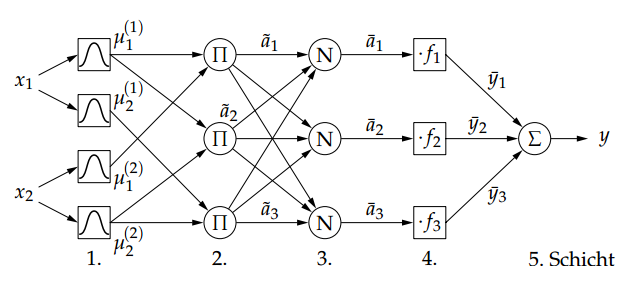
\includegraphics[scale=0.5]{images/ANFIS_Abb.png}
	\caption{ANFIS-Model \cite{CIKruse:15}}\label{ANFIS_Abb}
\end{figure}

In der \textbf{ersten Schicht} werden die Eingabewerte eingereicht und entsprechend die Zugehörigkeiten zu den Fuzzy-Sets ausgegeben. Weiterhin werden in der \textbf{zweiten Schicht} die Aktivierungswerte jeder Regel ausgewertet. Die Neuronen werden mit $\prod$ gekennzeichnet. Einzelnen Fuzzyzugehörigkeitswerte werden mittels Operatoren kombiniert, um die Aktivierungsgrad jeder Regel zu berechnen. Hier dürfen Operatoren zur Verknüpfung von Fuzzy-Mengen eingesetzt werden, üblicherweise der UND-Operator (siehe \ref{AND}). Die Gleichung \ref{eq3_3} ergibt die Berechnung bei gegebener UND-Verknüpfung:

\begin{equation}\label{eq3_3}
	\tilde{w}_i = \prod \mu_i^j(x_j)
\end{equation}

Die Variable $\tilde{w}_i$ ergibt die Aktivierung, oder Erf\"{u}llungsgrad, des Regels $R_i$ und $\mu_i^j$ ist die $j.$ Zugehörigkeitsfunktion in der Regel $R_i$.

Im \textbf{dritten Schicht} findet die Normalisierung aller Aktivierungswerte $\tilde{w}_i$ statt. Mit einfachen Worten wird der Beitrag berechnet, den jeder Regel für den Gesamtausgabe beiträgt. Nach der Normalisierung erhält man Aktivierungsgrößen zwischen $0$ und $1$. Die Gleichung \ref{barwi} berechnet die normalisierten Werten für jeden Regel $R_i$:

\begin{equation}\label{barwi}
\bar{w}_i = \frac{\tilde{w}_i }{\sum_j \tilde{w}_j } 
\end{equation}

Im \textbf{vierten Schicht} berechnen die mit $N$ markierten Neuronen die gewichteten Ausgabewerte. Das ``Gewicht'' (Ergebnis) aus dem letzten Layer wird mit der entsprechenden Ausgabefunktion multipliziert:

\begin{equation}
\bar{y}_i = net_i = \bar{w}_i\cdot f_i(x_1, ..., x_n). 
\end{equation}

Im \textbf{fünften Schicht} steht ein einziges Neuron, der mit $\sum$ beschriftet ist. Im letzten Schicht berechet man die Ausgabe, indem alle Werte aus dem \textbf{vierten Schicht} zusammenaddiert werden:

\begin{equation}
y = y_{out} = \sum_i \bar{y}_i = \frac{\tilde{w}_i\cdot f_i(x_1, ..., x_n)}{\sum_j \tilde{w}_j}.
\end{equation}

Diese Struktur ähnelt sich der von TSK-Modell. Für die Optimierung von Parametern der Zugehörigkeitsfunktionen und Konklusionsfunktionen eignet sich der ANFIS-Ansatz.

Das ANFIS-Modell ermöglicht die Optimierung von Modellparametern - die Fuzzy-Mengen- und Ausgabefunktionsparametern. Diese können erlernt werden, wenn eine angemessene Lernaufgabe vorliegt. Außerdem muss eine ausreichende Menge von Ein-/Ausgabe-Werten zur Verfügung stehen. Es bieten sich mehrere Lernmethoden zur Optimierung der Parametern. Zwei davon sind Gradientenverfahren(analog zur Fehler-Rückpropagation-Verfahren aus Neuronalen Netzen) und die Kleinste-Quadrate-Methode. \cite{CIKruse:15} \cite{Jang:93}

\subsection{Modell mit verstärkendem Lernen}

Bei Modellen mit verstärkendem Lernen wird versucht, die Menge der Daten für das Lernen möglichst gering zu halten. Der Unterschied zwischen Modell mit verstärkendem Lernen und solchen für feste Lernaufgaben besteht darin, dass bei dem Erstgenannten keine Vorwissen bekannt werden müssen, was öfters der Fall sein kann. Es reicht nur, wenn im Laufe des Lernens angegeben wird, ob die Richtung der Optimierung sinnvoll ist.

Ein großes Problem beim verstärkendem Lernen besteht darin, vorzusagen, wie groß der Einfluss einer Regelaktion auf das Gesamtsystem ist. Dieses Problem wird als \textit{Credit Assignment Problem} bezeichnet.

Es existiert eine große Mengen von Modelln mit verstärkendem Lernen, alle aber basieren auf dem gleichen Prinzip. Das System wird zwei Teilsysteme aufgeteilt: zum einen der ``Kritiker''(das ``kritisierende'' System) und der Aktor(zuständig für die Anwendung und Abspeicherung der Regelungsstrategie). Der Kritiker ``äußert'' seine Meinung über den jetzigen Zustand unter Berücksichtigung der vorhergehenden Zustände und somit entscheidet der Aktor anhand der Bewertung, ob eine Korrektur der Regelbasis gemacht werden soll. \cite{CIKruse:15}  \cite{UNIMAG:97}

\subsubsection{Das NEFCON-Modell}

Ziel des NEFCON-Modell, Neuro-Fuzzy Control Modell, ist es, eine interpretierbare Fuzzy-Regelbasis mit möglichst kleinen Trainingsschritten zu erlernen. Das Modell unterscheidet sich von dem ANFIS, indem es erlaubt einen Regelbasis, ohne Vorwissen zu erlernen. Dieses Modell bietet natürlich auch die Möglichkeit, Vorwissen mitzubringen. Das heißt sowohl Fuzzy-Systeme mit vorhandenen Regelbasis, als auch solche mit unvollständiger Fuzzy-Regelbasis. Alle diese Vorteilen sprechen für das NEFCON gegenüber andere Modelle.

Das NEFCON-Modell basiert auf ein Mamdani-Regler. Zum Veranschaulichung wird hier einen kleinen Beispiel mit Grafik \ref{NEFCON_Abb} und Regelbasis gegeben. \cite{CIKruse:15}

\begin{figure}[htbp]
	\centering
	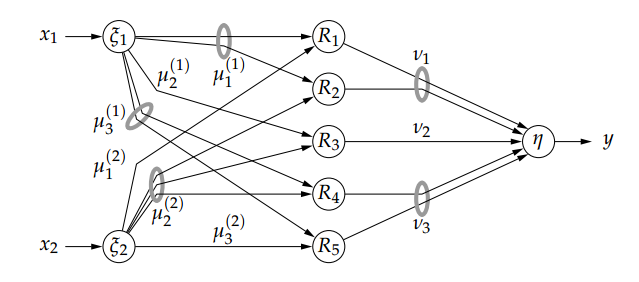
\includegraphics[scale=0.5]{images/nefcon_abb.png}
	\caption{NEFCON-Modell \cite{CIKruse:15}}\label{NEFCON_Abb}
\end{figure}

\begin{center}\label{nef_regelbasis}
	$R_1$: IF $x_1$ in $A_1^{(1)}$ AND $x_2$ in $A_1^{(2)}$, THEN y is $B_1$ \\
	$R_2$: IF $x_1$ in $A_1^{(1)}$ AND $x_2$ in $A_2^{(2)}$, THEN y is $B_1$ \\
	
	$R_3$: IF $x_1$ in $A_2^{(1)}$ AND $x_2$ in $A_2^{(2)}$, THEN y is $B_2$\\
	
	$R_4$: IF $x_1$ in $A_3^{(1)}$ AND $x_2$ in $A_2^{(2)}$, THEN y is $B_3$\\
	
	$R_4$: IF $x_1$ in $A_3^{(1)}$ AND $x_2$ in $A_3^{(2)}$, THEN y is $B_3$
\end{center} 

% Hier Grafik einfügen

Das NEFCON-Modell basiert auf einem generischen Fuzzy-Perzeptron. Das Modell konnte in drei Schichten aufgeteilt werden. Die \textit{erste Schicht} besteht natürlich aus den Eingangsneuronen. Die ist eindeutig und will nicht weiter darauf eingehen. In der \textit{zweiten Schicht} befinden sich die inneren Neuronen, die die Regeln einer Fuzzy-System widerspiegeln. Im Beispiel sind insgesamt fünf Regeln gegeben. Die Fuzzy-Mengen $\mu_r^{(i)}$, die in Mehrere Regeln vorhanden sind, werden durch Ellipse zusammengeführt. Falls beim Lernen eine Anpassung an einem Gewicht durchgeführt werden soll, muss dies in allen Verbindungen gemacht werden, wo die Menge figuriert.

Der eigentliche Lernprozess besteht aus zwei Phasen. In der erste Phase wird versucht, eine Regelbasis erlernt zu werden. Diese Phase wurde weggelassen, falls schon eine existiert. Es lassen sich auch unvollständige sogar fehlende Regelbasen lernen. Für das Letztere ist ein weiterer Algorithmus erforderlich.

In der zweiten Phase findet die Optimierung statt. Dabei werden Fuzzy-Sets modifiziert oder selbst die Verbindungen zu den Regeln umgetauscht. In dem NEFCON-Modell wird als Bewertungsmaß, der ``Kritiker'', ein Fuzzy-Error verwendet. Damit die Optimierung optimal ausgeführt werden kann, sollte das Vorzeichen des Ausgabewertes bekannt sein. Darüber hinaus wird ein erweiterter Fuzzy-Error $E^*$ berechnet:
	\begin{equation}\label{EFE}
	E^* = sgn(y_{out})\cdot E(x_1, \ \ldots , \ x_n)
	\end{equation}
\cite{CIKruse:15} \cite{UNIMAG:97}
\subsubsection{Erlernen einer Regelbasis}

Es existieren mehrere Algorithmen zum Erlernen von Regelbasis. Die Methoden können in drei Kategorien aufgeteilt werden: solche, die ohne vordefinierte Regelbasis startet; solche mit vollständiger Regelbasis und solche mit zufälliger Basis  starten. In den folgenden zwei Unterkapiteln werden Methode für die ersten zwei Kategorien vorgestellt. Bei den Methoden wird keine feste Lernaufgabe benötigt. Tatsächlich geht es darum, dass eine Initialbasis aufgebaut wird, ohne eine große Datenmenge mit optimalen Werten bekannt zu sein. \cite{CIKruse:15} \cite{UNIMAG:97}% Bis Hier drübergeguckt

\subsubsection{Top-Down- oder Reduktionsmethode zum Erlernen einer Regelbasis}

Zum Einen wird die Methode der Top-Down-Methode (in der Literatur auch als NEFCON I bekannt) genannt. Das Verfahren erfordt, dass eine vollständige Regelbasis vorhanden ist. Die Regelbasis beinhaltet auch widersprüchliche Regeln, die in Laufe des Prozesses ausgefiltert werden.

Der Prozess kann in zwei Phasen aufgeteilt werden. In der ersten Phase werden alle die Regeln eliminiert, die bei ihrer Ausgabe den falschen Vorzeichen aufweisen. Die auszufilternden Regeln werden mit der erweiterten Fuzzy-Fehler-Funktion (siehe \ref{EFE}) bestimmt. In der zweiten Phase werden Regeln mit identischer Prämisse zufällig ausgewählt. Folglich wird der Fehler für die bestimmte Regel berechnet. Zum Schluss wird die Regel ausgewählt, die die kleinste Fehlerrate aufweist. Die restlichen Regeln werden verworfen.

Eins der Nachteile der Top-Down-Methode ist die Aufwändigkeit, weil es mit einer großen Regelbasis gestartet wird. Das nächste Verfahren ist das Gegenteil von Top-Down-Methode, zwar Bottom-Up-Methode. \cite{CIKruse:15}


\subsubsection{Bottom-Up- oder Eliminationsmethode zum Erlernen einer Regelbasis}

Der Bottom-Up-Algorithmus beginnt mit einer leeren Regelbasis. Jedoch muss eine initiale Aufteilung(Intervall) der Ein- und Ausgabewerten gegeben sein. Analog zur Top-Down besteht diese Methode auch aus zwei Phasen. 

Erste Phase beginnt mit der Bestimmung der Prämisse für die Regeln. Der Prozess evaluiert jede Fuzzy-Menge mit bestimmten Eingaben und die Mengen, die den höchsten Zugehörigkeitsgrad aufweisen, werden ausgewählt. Aus den ausgewählten Fuzzy-Mengen werden neue Regeln gebaut. Danach versucht der Algorithmus eine geeignete Ausgabe aus dem aktuellen Fuzzy-Fehler zu ``raten''. Dabei wird vorausgesetzt, dass Eingaben mit ähnlichen Fehlerwerten ähnliche Ausgaben liefern.

In der zweiten Phase werden die Fuzzy-Mengen in den Konklusionen optimiert. Dabei werden nicht die Parametern der Konklusionen angepasst, sondern bei Bedarf die Fuzzy-Menge durch eine andere ersetzt.

Wegen des inkrementellen Lernen lässt sich einfach Vorwissen in dem Regelbasis einführen. Bei den Fällen mit unvollständigen Regelbasen werden passende Regeln hinzugefügt. Das Verfahren garantiert jedoch nicht, dass immer eine geeignete Regelbasis aufgebaut wird. Aus diesem Grund ist es empfohlen, dass die Regelbasis manuell am Ende des Lernens überprüft und entsprechend angepasst wird. \cite{CIKruse:15} \cite{UNIMAG:97}

\subsubsection{Optimierung der Regelbasis}

Die Optimierung bei NEFCON verwendet die Methode ``Back Propagtion Method'', oder Rückpropagationsmethode. Der Fehler wird rückwirkend durch das Netz geführt und lokal bei jeder Fuzzy-Menge angewendet.

Eine Änderung darf sowohl in den Prämissen, als auch in den Konklusionen. Es wird das Prinzip des verstärkenden Lernens angewendet. Das bedeutet, dass für jede Änderung eine Fuzzy-Menge entweder ``bestraft'' oder ``belohnt'' wird. Bestrafung und Belohnung werde in Änderungen wie Verschiebung, Vergrößerung oder Verkleinerung des Bereichs einer Fuzzy-Menge ausgedrückt. Änderungen werden entsprechend iterativ in Beziehung zum Fuzzy-Fehler gemacht. \cite{CIKruse:15} \cite{UNIMAG:97}

\subsubsection{Schlussworte}

% Zusammenfassung der zwei Methoden,
Die Methoden unterscheiden sich in ihrem Kern kaum. Beide Architekturen besitzen entsprechend Vorteile und Nachteile. Der größte Unterschied liegt in der Ausbau ihrer Struktur. ANFIS basiert auf TSK-Modellen, währen NEFCON auf die Mamdani-Reglern. Beide Modelle bieten sie sich gut für das Lernen von Fuzzy-Systeme, jedoch entspricht nur das ANFIS meinem Anwendungsfall - Optimierung von TSK-Modelle.
\chapter{Neuro-Fuzzy-Modelle: Implementierung des ANFIS-Ansatzes}

In der folgenden Kapitel stelle ich die Aufsetzung des ANFIS-Ansatzes in Python vor. Während der Ausarbeitungszeit habe ich mich mit der Bibliothek für Neuronale Netze Tensorflow gesetzt. Tensorflow ist ein Produkt von Google und eine API für Erstellung von Neuronalen Netzen. Eine weitere Funktionalität, die die Bibliothek anbietet, ist die einfache Migration von erstellten Neuronalen Netzen. Tensorflow bietet die Möglichkeit, einfach Modelle nach den unterstützten Programmiersprachen zu exportieren, in disem Sinne auch nach C++.

In diesem Kapitel wird so vorgegangen, dass zu jedem Programmcode eine Erklärung gegeben wird. Der vorrige Kapitel geht auf die eigentliche Struktur und theoretische Aufsetzung eines ANFIS-Models in einem Neuronalen Netz. Laut dem Kapitel \ref{ANFIS} besteht ein ANFIS-System aus sechs Schichten (zwei äußere und vier inneren Schichten). Über die erste Schicht erfolgt die Eingabe im Netz. Die weiteren fünf Schichten führen einfache mathematische Funktionen aus.

\section{ANFIS-Klasse}\label{anfis-klasse}

Das Neuro-Fuzzy-Model wird nach dem bekannten ANFIS-Model eingerichtet. Das Model hat insgesammt 6 Schichten, 2 Außen- und 4 Innenschichten. Das ANFIS-Model wird in einer Klassendatei ausgelagert. Die Klasse verfügt über mehrere Methoden, einige davon Hilfsmethoden. Folglich werden die Wichtigsten davon in Unterkapiteln gestellt.
\subsection{Konstruktor}\label{konstruktor}

Die ANFIS-Klasse vefügt über einen einzigen Konstruktor. 

\begin{lstlisting}[language=Python]
# gradient_type defines the batch size to be used for learning
# 0-type = Stochastic Gradient Descent
# 1-type = Mini-Batch Gradient Descent, 30 samples from the training data
# 2-type = Batch Gradient Descent
def __init__(self, num_sets, path=None, gradient_type=0, mf_type=0):
...
\end{lstlisting}

Er hat einen Pflicht- und drei Optionalparameter - \emph{num\_sets} und entsprechend \emph{path}, \emph{mf\_type}, \emph{gradient\_type}. Der Parameter \emph{num\_sets} besagt wie viele Fuzzy-Mengen pro Eingangsgröße zu erstellen sind. Der Pfad wird durch ein String - \emph{path} - gegeben. Weiterhin unterscheide ich zwischen zwei Weisen der Berechnung von Zugehörigkeit. Anschliesend ergibt die Variable \emph{gradient\_type} die Größe der Trainingsdaten, oder die Art des Gradient-Descents. Es unterscheiden sich drei Arten von Gradient Descent Verfahren -
Stochastic, Mini-Batch und Batch Gradient Descent Verfahren. Die gegebene Anordnung der Begriffe entspricht der in dem Programmcode, sprich \emph{gradient\_type=0} entspricht dem stochastischen Verfahren. Der Wert \emph{1} heißt, dass das Mini-Batch ausgewählt wird und \emph{2} - Batch Gradient Descent. Die drei Arten unterscheiden sich in dem Punkt, dass die Variablen zu Unterschiedlichen Zeitpunkten angepasst werden. Bei dem stochastischen Verfahren werden die Parameter nach jeder Bearbeitung von Trainingspaaren verändert. Bei dem Mini-Batch wird jeweils nach der Bearbeitung von gewisser Anzahl an Datenelementen. Eine übliche Anzahl ist meistens zwischen 30 und 500 Trainingsdaten pro Iteration, jedoch ist das weniger als der Gesamtmenge. Der Batch Gradient Verfahren nimmt die ganze Datenmenge und führt mit denen einen Lernzug. Die Erkenntnisse aus den Tests werde ich in dem nächsten Kapitel beschreiben.

Der Konstruktor umfasst Definition der benötigten Variablen und die Erstellung des Models. Zu beginn werden die Trainingsdaten aus einer Datei gelesen. Durch die Struktur des Datensatzes wird die Anzahl der Eingangvariablen in dem Netz bestimmt. Die Datenpaar sind zeileinweise aufgebaut. In der Zeile werden zu bestimten Eingaben die Soll-Ergebnisse gegeben. Die letzte Spalte liefert die Sollwerte und in den Spalten davor werden die Eingangswerte geschrieben, sodass zum Beispiel in der ersten Spalte \(\mathbf{x_1}\), in der zweiten \(\mathbf{x_2}\) usw. und in der letzen der Erwartungswert steht. Üblicherweise arbeite ich mit einer Eingangsgröße, somit hat eine Datei zwei Spalten. 
Falls das gegebene Pfad gültig ist, werden vier Felder erstellt, zwei jeweils fürs Lernen und die Prüfung. Falls der Parameter \(\textit{fulltrain}\) auf \(\textit{wahr}\) gesetzt ist, werden die Daten nicht aufgeteilt. Bei dem Vorderen werden die Daten so getrennt, dass drei viertel der Datensätze fürs Training und ein viertel der Daten für die Bewertung des gelernten Modells verwendet werden. 
Anschließend wird mit der Konstruktion des Neuronalen Netzes fortgefahren. Folglich werden sechs weiteren Hilfsmethoden ausgeführt, die die Schichten des Neuronalen Netzes ausbauen. Diese werde ich etwas ausführlicher vorstellen.

Ein Beispiel für einen Aufruf des Konstruktors:

\begin{lstlisting}[language=Python]
#...
# the default mf_type and gradient_type 
# are set to 0, although gradient_type 0 is not the most optimal
f = Anfis(num_sets=num_sets, 
	path="../utils/sinus.out", gradient_type=0, mf_type=0)
\end{lstlisting}

\subsection{Eingangsschicht (FirstLayer)}\label{eingangsschicht-first-layer}

Die Definition der Eingangsschicht erfolgt in der Funktion \emph{first\_layer()}. Die Methode erhält keine Parameter und initialisiert zwei Tensoren für die Eingangsgrößen \textbf{X} und \textbf{Y}. In Tensorflow können Eingaben an mehreren Stellen im Netzt eingeführt werden, was hier auch der Fall für die \textbf{Y-Variable} ist. Die \textbf{Y-Variable} wird in der Fehlerfunktion gebraucht und sie enthält alle Soll-Ergebnisse.


\begin{lstlisting}[language=Python]
#...
# three different types for gradient descent type
# so we have three types of batch size, 
# wich defines the amount of elements to be evaluated in one iteration
if self.gradient_type == 0:
	self.batch_size = self.num_inputs
elif self.gradient_type == 1:
	self.batch_size = int((1 / 5) * (len(self.train_x_arr)))  
elif self.gradient_type == 2:
	self.batch_size = len(self.train_x_arr)
# input variable
self.x = tf.placeholder(name="x", shape=(self.num_inputs, self.batch_size), 
	dtype=tf.float64)
# variable for expected result
# we define dtype=tf.float64, because of the size of the values
# that the model returns
self.y = tf.placeholder(name="y", shape=(self.batch_size), dtype=tf.float64)
#...
\end{lstlisting}

Die $\textbf{Variable X}$ ist ein Array, das eine Matrix mit $\textit{n (num\_inputs)}$ Zeilen (Werten) und $\textit{batch\_size}$ Spalten repräsentiert. Die Methode $\textit{placeholder}$ in Tensorflow erstellt einen Tensor, der keine zusätzliche Operation oder Funktion ausführt. $\textit{Placeholders}$ werden meistens als Eingangsvariablen verwendet. In der Variable $\textit{num\_inputs}$ wird die Anzahl der Eingangsvariablen geschrieben. Im normalen Fall entspricht der Wert von $\textit{n}$ gleich 1. Weitere Größen für $\textit{n}$ werden nicht betrachtet. Der $\textbf{Y-Placeholder}$ wird auch als Eingabe in dem Verlustfunktion genutzt, die später in dem Unterkapitel \ref{optimisierungsfunktion} gegeben wird. Der $\textbf{Tensor Y}$ enthält am Ende einer Iteration den Erwartungwert für gegebener $\textbf{Eingangswert X}$. Der eigentliche
Ausgangswert(Istwert) wird von der letzen Schicht berechnet.

\subsection{Konklusionsparameter}\label{konklusionsparameter}

Nach der Definition der Eingangsvariablen erfolgt die Erstellung von zwei Variablen, in denen die Konklusionsparametern gespeichert werden. In diesem Fall handelt es sich nicht mehr um $\textit{Placeholdern}$, sondern $\textit{Variablen}$. Ihre Konstruktion erfolgt über die Hilfsfunktion $\textit{get\_variables()}$. Die Funktion überprüft, ob eine Variable mit gegebener Name existiert. Variable wird erstellt, wenn das nicht der Fall ist, ansonsten wird die entsprechende Variable zurückgeliefert.

Im Kapitel 1 und in 2 aus der Dokumentation ist der Normalform der Konklusionsfunktionen eines Takagi-Sugeno-Kang-Modells definiert. Die Form der Gleichung ist hier nochmal gegeben:

\begin{align}
f_i(x_1, ..., x_m) & = w_0^i + w_1^i\cdot x_1 + ... w_m^i\cdot x_m
\label{konk_func}
\end{align}
Jede Konklusionsfunktion hat ihre eigene Parameter. Damit keine einzelnen Variablen definiert werden, können diese in einem Vektor, bzw. Matrix, gespeichert werden. Die Stelligkeit der ersten Variable $w_0^i$ in der Gleichung \ref{konk_func} hängt von der Anzahl der Regeln. Wir rechnen mit insgesammt $num\_sets^{num\_inputs}$-Viele Regeln ($\textit{num\_rules}$). Für die restlichen Konklusionsparametern $w_y^i$ wird eine Matrix mit Dimensionen $num\_rules\times num\_inputs$ erstellt. Beide Variablen sind trainierbar, was aus dem Parameter $\textit{trainable}$ ersichtlich wird. Folgendes Programmabschnitt stellt die Umsetzung dar.

\begin{lstlisting}[language=Python]
#...
	self.a_0 = tf.get_variable(name="a_0", dtype=tf.float64,
	initializer=np.ones(shape=(self.num_rules, 1)), trainable=1)
	self.a_y = tf.get_variable(name="a_y", dtype=tf.float64, 
	initializer=np.ones(shape=(self.num_rules, self.num_inputs)), 
trainable=1)
#...
\end{lstlisting}

\subsection{Zugehörigkeitsfunktion (Second and Third Layer)}\label{zugehuxf6rigkeitsfunktion-second-and-third-layer}

Die erste Aufgabe sei die Definition der
\textbf{Zugehörigkeitsfunktionen (ZGF)}. Die Gesamtzahl der ZGFs ergibt
sich aus dem Produkt der beiden Werten für Anzahl Fuzzy-Sets und
Eingangsgrößen (\(\textit{num\_sets}\) und \(\textit{num\_inputs}\)). Die
Erstellungsmethode wird \(\textit{mfs()}\) genannt. Zwei Operationen
werden in der Funktion ausgeführt - Erstellung der einzelnen ZGF und
deren Kombination in Premissen.

\subsubsection{Definition in Tensors aller Zugehörigkeitsfunktionen}\label{definition-in-tensors-aller-zugehuxf6rigkeitsfunktionen}

In meinem Projektes habe ich mich nur mit Dreiecksfunktionen
beschäftigt, in der Dokumentation werden weitere
Zugehörigkeitsfunktionen vorgestellt. Wie die Name verraten würde,
stellt die Dreiecksfunktion einen Bereich, der durch drei Punkten
aufgespannt ist, dar. In der Methode \(\textit{second\_layer}\) werden
zuerst alle Funktionsparametern iterativ mit einem Wert erstellt. Jeder
Parameter wird in einem trainierbaren Tensor gespeichert. Dies erfolgt
über die Hilffunktion \(\textit{triangular\_mf}\), die entsprechend so
aussieht:
\begin{lstlisting}[language=Python]
def triangular_mf(self, x, par, name):
	# we define the triangular function
	if self.mf_type == 0:
	# we split the traingular space into two
	# the left side
	# we calculate the membership of x to the left side
	# we get a negative value if x is not part of the space
		dividend_left = tf.subtract(x, par[0])
		divider_left = tf.subtract(par[1], par[0])
		division_left = tf.divide(dividend_left, divider_left)
	# we calculate the membership of x to the right side
		dividend_right = tf.subtract(par[2], x)
		divider_right = tf.subtract(par[2], par[1])
		division_right = tf.divide(dividend_right, divider_right)
	# we get the lowest value
		minim = tf.minimum(division_left, division_right)
	# then we calculate the highest of 0 and the previous value
		maxim = tf.maximum(minim, tf.cast(0.0, tf.float64))
	elif self.mf_type==1:
	# first we calculate the dividend. We subtract the middle parameter 
	#of the mf with x
	dividend = tf.abs(tf.subtract(par[1], x))
	# then we subtract the two boundary parameters of the membership function
		divider = tf.subtract(par[2], par[0])
	# we divide the two values to get the output of the memberhip function
		op = tf.divide(dividend, divider)
	# then we multiply it by 2, because we devide it by the whole length of
	#the triangle
	# and not just half of the length.
		mul = tf.multiply(tf.cast([2.], tf.float64), op)
	# we subtract 1 from it so we always either have a positive value when x
	#is a member
	# of the set, or we get a negative value
		sub = tf.subtract(tf.cast([1.], tf.float64), mul)
	# we calculate the maximum of the value from the mf and 0, this way we
	#don't take variables that are outside
	# the range of the membership function
		maxim = tf.maximum(tf.cast([0.], tf.float64), sub, name=name)
	return maxim

\end{lstlisting}

Die Hilfsfunktion \(\textit{triangular\_mf()}\) nimmt drei Argumente ein. Die \emph{Variable x} kann mehrere Einträge repräsentieren, abgesehen davon welcher Art der Gradienten Verfahren verwendet wird. Der zweite Methodenparameter speichert in sich die davor definierten Funktionsparametern. Schließlich wird eine Name als String gegeben. Jede Funktionsname ist eindeutig gewählt, so dass auf jede Funktion bei Bedarf über die \(\textit{get\_variable()}\)-Methode zugegriffen werden kann. Außerdem vereinfacht die Namensetzung das Debugging, weil alle Variablen eindeuting sind.

\subsubsection{Erster Programmteil (Second Layer)}\label{erster-programmteil-second-layer}

Im ersten Teil der Methode \(\textit{second\_layer()}\) erlangt die Definition aller Fuzzymengenparametern. Ich habe mich für diese Vorgehensweise entschieden, da die getrennte Erstellung der Variablen ermöglicht, dass jeder Parameter spezifisch definiert ist. Auf dieser Weise könnte ich mehr Einfluß auf einzelnen Ergebnisse und Vorgänge haben.

\begin{algorithm}
	\caption{Definition of Fuzzy member parameters}
	\begin{algorithmic}[1]
		\REQUIRE $value\_scope$
		\ENSURE $val\_inc \leftarrow increment$
		\FORALL{$par$}
			\IF{$index\equal 0$}
				\STATE $par \leftarrow tensor(val=value\_scope[0],$ $trainable=0)$
			\ELSIF{$index\equal last$}
				\STATE $par \leftarrow tensor(val=value\_scope[1],$ $trainable=0)$
			\ELSE
				\STATE $par \leftarrow tensor(val\_inc)$
				\STATE increment $val\_inc$	
			\ENDIF
		\ENDFOR
 	\end{algorithmic}
\end{algorithm}

Das Pseudocode beschreibt die Erstellung eines Parameters. Es wird unterschieden, welcher Parameter definiert wird. Die ersten und letzen Parameter sind nicht trainierbar, um Definitionslücken zu verhindern.

Es wurde schon erwähnt, dass alle Parametern aufsteigend angeordnet sind. Aus der Abbildung \ref{mfs_urs} wird ersichtlich, wie diese Parametern, insbesondere die ZGF, am Anfang aussehen.

\begin{figure}
	\centering
	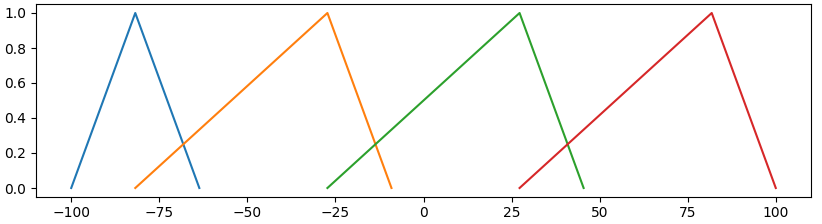
\includegraphics[scale=0.5]{images/mf_with_parameters.png}
	\caption{Ursprüngliche Fuzzy-Mengen}
	\label{mfs_urs}
\end{figure}

Die Anordnung ist gleich bei allen Mengen außer die Erste. Damit keine
Definitionslücken entstehen, verzichte ich auf die Trainierung der
beiden Grenzwertparametern. Neben dem Trainingsausschluß des ersten
Parameter der ersten Menge und des letzten der letzen Mengen, die die
Wertebereich bestimmen, werden auch weitere Einschränkungen angelegt.
Zum einen wird der Wert der Spitzenparameter (mittlerer Parameter) jeder
Funktion begrenzt, sodass er nicht kleiner als der linke Parameter, bzw.
größer als der rechte Parameter, wird. Der Spitzenparameter darf nicht gleich der linke oder rechte Parameter sein, weil es zur Undefiniertheit der Zugehörigkeitsfunktion führt.

Infolge des Austesten tauchten kritischen Fehler bezüglich der
Undefiniertheit der Zugehörigkeitsfunktionen auf. Diese Mangeln könnte
ich mit drei Einschränkungen aufheben. Die Beschränkungen fallen auf die
drei Parametern der Dreiecksfunktion.


\subsubsection{Zweiter Programmteil (Third Layer)}\label{zweiter-programmteil-third-layer}

Der zweite Programmteil enthält weniger Programmcode, aber dauert unter
Umständen länger. Die lange Laufzeit ergibt sich aus der Berechnung der
Permutationen der ZGF für alle Eingaben. Die Bibliothek
\(\textit{itertools}\) stellt mehrer Funktion bereit. Eine der Methoden
daraus berechnet das kartesische Produkt. Die Funktion kann mehrere
Mengen und einen \textbf{repeat}-Parameter entgegennehmen und liefert
eine Ergebnismenge. Die \textbf{repeat}-Variable gibt an, wie oft das
kartesische Produkt ausgeführt wird. Die Iteratorfunktion ist in der
Komplexitätsklasse \(TIME_{product()} \in O(n^k)\), mit \emph{n} gleich
die Anzahl der Elemente in der Angegebene Menge und \emph{k} gleich die
Anzahl der Ausführungen. Ein kleines Beispiel zur Verdeutlichung als
auch eine Implementierung des zweiten Programmteils wird unten gegeben.

\begin{lstlisting}[language=Python]
# itertools.product(l, r) builds the cartesian product of 
#the iterables (the list l).
# if r is equal to two, this would return the cartesian product 
#of the list l with itself (l x l).
# if r is three - (l x l x l). We use it here to get all 
#the combinations between the inputs
# Example: product((A, B), repeat=2) would result in the 
#list [(A, A), (A, B), (B, A), (B, B)]
for perm in it.product(range(self.num_sets), repeat=self.num_inputs):
	tmp = tf.ones(shape=(), dtype=tf.float64)
# loop from 0 to self.num_inputs and multiply the MF of an 
#input with index perm[i] with every other MF 
#with index from the permutation list
	for i in range(len(perm)):
		tmp = tf.multiply(premises[i][perm[i]], tmp)
	self.mf[index] = tmp
	index += 1
end = t.process_time()
\end{lstlisting}

Aus der Komplexitätsklasse ergibt sich, wie oft die äußere Schleife ausgeführt wird. Genauer gesagt, der Loop braucht so viele Iterationen bis zum Schluss wie die Gesamtzahl der Regeln. In der innere Schleife werden die Elemente in der Liste durchlaufen. Pro Iteration wird ein Element aus der Productliste betrachtet. Jeder Eintrag aus der Liste repräsentiert ein Index \textbf{perm{[}i{]}} einer Zugehörigkeitsfunktion für die entsprechende Eingabe \textbf{i}. Die Funktionen werden der Reihe nach mit einem Dummy-Tensor multiplizert. Auf dieser Weise werden die Prämisse jeder Regel definiert.

\subsection{Fourth Layer}\label{fourth-layer}

Im dritten Layer laut der Struktur des ANFIS-Models, werden alle Ergebnisse aus dem vorrigen Schicht normiert. Die Funktion besteht nur aus zwei Zeilen Code:
\begin{lstlisting}[language=Python]
def third_layer(self):
	# Reshape the MFs
	# Reshape the array, to be in the form of an array with 
	#num_rules items in it
	# sum the elements in the array along the 0th dimension
	self.mf_sum = tf.reduce_sum(tf.add(self.mf, [1e-10]), 0)
	# Normalize the MFs
	# Add all the items in the vector and divide every item in 
	#it with the sum of the elements
	# This way we get the normalized membership functions
	self.normalizedMFs = tf.divide(self.mf, self.mf_sum)
\end{lstlisting}

Mit der Funktion $\textbf{reduce\_sum()}$ werden die Einträge in einem Array, bzw. Matrix oder Vektor, zusammensumiert. Es kann einen zusätzlichen Parameter angegeben werden, der in der Dokumentation als $\textbf{axis}$ beschriftet ist und der angibt, welche Achse entlang die Elemente summiert werden sollen. Wie man am oberen Programmcode erkennt, werden hier die Elemente die 0. Achse entlang summiert. Wenn wir eine Matrix betrachten würden, heißt das für die Summe, dass die Elemente in einer Spalte summiert werden. Das Ergebnis der Summierung wird entsprechend in einer Variable abgespeichert, da wir einen zwei-Dimensionalen Array mit jeweils einen Eintrag in der zweite Dimension, erhalten wir eine Zahl. Schließlich werden alle Zugehörigkeitsfunktionen durch diesen Wert geteilt. Auf diesem Weg wird das Ergebnis der Prämissen normiert und ihre Summe gleich $\emph{1}$.

\subsection{Fifth Layer}\label{fifth-layer}

Die fünfte Schicht soll das Ergebnis aus jeder Konklusionsfunktion berechnen. Die Ausgabe erhalten wird, in dem die Eingangsgrößen in jeden Konklusionsfunktion eingesetzt werden und der Zutriffswert der Regeln an dem Funktionswert multipliziert werden. Durch die Normalisierung der Eintretungsgrößen erhalten wir eine Summe der Gewichte von 1, also ein Ergebnis mit Faktor kleiner 1 wird ausgegeben.

\begin{lstlisting}[language=Python]
def fifth_layer(self):
	# multiply every premis with its coresponding conclusion function
	# we get a vektor of results with each result having a factor less than 1
	self.outputs = tf.multiply(self.normalizedMFs, self.conclusions)
\end{lstlisting}

\subsection{Sixth Layer}\label{sixth-layer}

Die Summe aller Werten und das eigentliche Ergebnis für ein gegebenes Kandidat $\textbf{X}$ wird in der letzen (sechsten) Schicht berechnet. Dies erfolgt in einem Einzeiler:

\begin{lstlisting}[language=Python]
def sixth_layer(self):
	self.result = tf.reduce_sum(self.outputs, 0)
\end{lstlisting}

\section{Optimisierungsfunktion}\label{optimisierungsfunktion}

Nachdem das Neuronale Model aufgebaut wird, folgt die Definition des Optimierungsverfahren. In der Literatur, auch in der Praxis, wird die Kleinste-Quadrate Funktion verwendet. Auch hier habe ich diese eingesetzt. Als nächstes muss der Optimiser definiert werden. Die zwei bekanntesten sind $\emph{GradientDescentOptimizer}$ und $\emph{AdamOptimizer}$. Nach zahlreichem Testen der beidein Optimizer bin ich zu der überzeugung gekommen, dass der $\emph{AdamOptimizer}$ besser geeignet ist. Unten ist die Definition der Optimierungsfunktion gegeben.

\begin{lstlisting}[language=Python]
def optimize_method(self):
	self.loss = tf.losses.mean_squared_error(self.y, self.result)
	# self.loss = tf.losses.huber_loss(self.y, self.result)
	
	# self.optimizer =  
	#tf.train.GradientDescentOptimizer(learning_rate=0.01)
	#.minimize(self.loss)
	self.optimizer =
		 tf.train.AdamOptimizer(learning_rate=0.1).minimize(self.loss)
	# self.optimizer =
	# tf.train.RMSPropOptimizer(learning_rate=0.1).minimize(self.loss)
\end{lstlisting}
 
Wie üblich die Fehlerate ergibt sich aus dem Soll- und Istergebnis.
Weiterhin erhalten wir den Optimierer durch einen simplen Codeaufruf,
während dessen auch einen Lernrate gegeben wird. Normalerweise wird die
Lernrate mit einem Wert von 0.1 gesetzt.


\section{Trainingsfunktion}\label{trainingsfunktion}

Mit den oben erklärten Funktionen kann einen ANFIS-Model mit beliebigen
Eigenschaften erstellt werden. Nach dem Ausbau folgt das eigentliche
Lernen. Darum habe ich eine separate Methode definiert, die den Ablauf
beim Lernen beschreibt.
%\begin{lstlisting}
%	# PSEUDOCODE HERE
%	
%\end{lstlisting}

\begin{algorithm}
	\caption{Training function}
	\begin{algorithmic}[1]
		\REQUIRE initialize $statistic\_arrays$
		\STATE create $before\_training\_graphics$
		\IF{$gradient\_type\equal 0$}
			\STATE $train\_stocastic()$
		\ELSIF{$gradient\_type\equal 1$}
			\STATE $train\_mini\_batch()$
		\ELSE
			\STATE $train\_batch()$
		\ENDIF
		\STATE create $after\_training\_graphics$
		\STATE save data
	\end{algorithmic}
\end{algorithm}

Die Trainingsfunktion kann in vier Teile abgegrenzt werden. In dem ersten Teil fallen alle Operationen für die Aufzeichnung der Grafiken vor dem Lernen. Im zweiten Teil fällt der Lernzug. Danach kommt entsprechend die Zeichnung des 
geänderten Models. Zum Schluss werden alle Daten in Dateien abgespeichert.

Im nächsten Kapitel wird das beschriebene Programm getestet. Die Tests haben zum Ziel einen Verstand zu verschaffen, wie schell das Modell lernt und wie das Modell am besten konfiguriert werden kann.
\chapter{Analyse der Ergebnisse}

In diesem Kapitel findet man Informationen über die durchgeführten Programmtests. Ziel der Testfälle ist es zu bestimmen, wie gut meine Implementierung des ANFIS-Models lernt. In jedem Unterkapitel wird gegen eine bestimmte Eigenschaft getestet. Bei der Untersuchung nehme ich in Betrachtung zwei mathematischen Funktionen, zwar die Parabel- und Sinusfunktion. 

Bei den Tests werden drei Arten von Gradient-Descent-Verfahren angesetzt - Stochastischen, Mini-Batch und Batch Gradienten Verfahren. Deren Eigenschaften werden in den nächsten Unterkapiteln erläutert. 

Außerdem werde ich zwei unterschiedlichen Berechnungsweisen für die Zugehörigkeitsfunktionen verwenden. Die zwei Arten nenne ich MF-Typ 0 und MF-Typ 1. Wenn ich vom MF-Typ 0, oder nur Typ 0, spreche, meine ich, dass die Zugehörigkeitsberechnung in zwei Teilen untergegliedert ist. Man kann das Dreieck, das durch die drei Parametern der Zugehörigkeitsfunktion bestimmt ist, durch die Mitte teilen. Dann entstehen zwei Bereiche, die separat betrachtet werden. Auf dieser Weise entstehen zwei Gleichungen (Teilen). Bei dem Typ 1 erfolgt die Berechnung in einer Gleichung. Also da wird nicht unterschieden, wo der X-Wert auf der Hypothenuse liegt - kleiner oder größer als der Mittelpunkt. Die zwei Berechnungsweisen für MF-Typ 0 \ref{mf_typ0} und MF-Typ 1 \ref{mf_typ1} gebe ich als Gesammtformel an.
\begin{align}
	\begin{split}\label{mf_typ0}
		\mu(x) = \max[\min(\frac{x - a}{m - a}, \frac{b - x}{b - m}), 0.0]
	\end{split}\\
	\begin{split}\label{mf_typ1} 
		\mu(x) = \max[0, 1 - 2\frac{\lvert x - m\rvert}{b - a}]
	\end{split} 
\end{align}
%H. Bothe, Neuro-Fuzzy-Methoden zweite Gleichung
Die erste Berechung ist von MF-Typ 0 und die Zweite von Typ 1. In der Gleichung sind die Größen \textit{a, m und b} die Parametern der Zugehörigkeitsfunktion. Die Variable \textit{a und b} sind die zwei Grenzwerte entsprechend links und rechts, und \textit{m} ist der Gipfelpunkt, oder Mittelpunkt.

Alle unseren Lerndaten werden aus einer Datei, die einen spezifischen Aufbau hat, gelesen. Die Daten können in zwei Gruppen aufgeteilt werden - Eingaben und Soll-Ergebnisse. Jede Spalte beinhaltet Elemente aus einer der beiden Gruppen, wobei die Letzte immer die Soll-Ergebnisse enthält. Da in diesem Projekt einstellige Funktionen in betracht genommen werden, gibt es in der Datei nur zwei Spalten.

Nachdem alle Verfahren vorgestellt wurden, wird mit den Tests begonnen.Wegen der größe Anzahl an Tests werden nur bestimmte ausgewählt. Eine Tabelle und alle Modellgrafiken werden später am Ende der Ausarbeitung angehängt. 

Die Vorgehensweise bei der Beschriftung der Testfälle erfolgt für beide Funktionen gleich. Für ein Model wird seine Struktur und seine Eigenschaften gegeben. Weiterhin wird das Ergebnisgrafik gezeichnet. Zum Schluss werden die gelernten Konklusionsfunktionen vorgestellt. Zu jedem Teil wird eine Erläuterung zusätzlich aufgeführt. 
 
\subsubsection{Stochastic Gradient Descent}
Bei dem stochastischen gradienten Verfahren (Stochastic Gradient Descent) handelt es sich um eine spezifische Eingabenweise. Bei dieser Vorgehensweise werden einzelnen Einträgen aus dem Datensatz als Eingabe in das Model gegeben. Somit beschreibt ein Element eine Iteration (Epoche) in dem Lernprozess. Nach jeder Iterationen werden die betroffenen Gewichten (Parametern) angepasst. \cite{SBMB:19}


\subsubsection{Mini-Batch Gradient Descent} \label{mini_batch}
Bei dem Mini-Batch Verfahren werden kleine Sets, normalerweise zwischen 30 und 500 Elemente, aus der Menge der Daten genommen und diese an dem Model zum Lernen gegeben. Das heißt eine Iterationen wird erst dann durchgeführt, wenn alle Elemente aus dem Batch abgearbeitet werden. Dieses Verfahren wird öfters bei Lernaufgaben verwendet, bei dennen der Datensatz extrem groß ist. In meinem Programm baue ich Zufälligkeit, sodass die Lernmenge zufällig aus der Gesamtmenge auszuwählen ist. \cite{SBMB:19}

\subsubsection{Batch Gradient Descent}\label{batch}
Bei dem Batch Gradient Descent setzt man eine Architektur, bei der alle Daten in dem Lernprozess innerhalb eines Lernzugs fließen. Diese Art ist gut geeignet, bei Problemstellungen, wo die Datenbasis angemessen groß ist. In unseren zwei Fällen handelt es sich um relativ kleine Datenmengen (400 und 1000 Datensätze entsprechend für Sinus- und Parabelfunktion). Bei Lernaufgaben mit 100 Tausende von Datensätze ist diese Vorgehensweise ungeeignet. Da ist das Mini-Batch-Verfahren einzusetzen. \cite{SBMB:19}

\section{Lernen der Sinusfunktion mit Stochastic Gradient Descent}
In diesem Kapitel wird die Sinusfunktion untersucht. Hier erläutere ich die Ergebnisse, die bei den Lernvorgängen erschaffen wurden. Zum Schluss verschaffe ich einen Überblick über die besten Eigenschaften zum Lernen der Sinusfunktion.

Die Sinusfunktion ist als Zeichnung (siehe \ref{sinus}) angegeben.

\begin{figure}
	\centering
	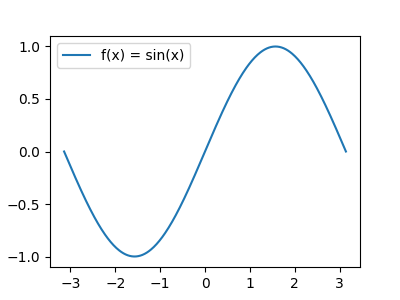
\includegraphics{images/sinus.png}
	\caption{Die  Sinusfunktion.}
	\label{sinus}
\end{figure} 

\subsubsection{Lernen eines Models mit 2 Fuzzy Sets und 1 Ablauf}

Anfangend lasse ich das Model einen Lauf durchführen. Wobei hier wichtig zu erwähnen ist, dass eine Iteration und ein Lauf nicht das selbe ist. Iteration im stochastischen Verfahren bedeutet, dass ein Element aus der Datenmenge verarbeitet wurde und ein Lauf - dass alle Elemente erarbeitet sind. Also heißt es für unsere Laufzeit, dass das Model bereits nach einem Lauf 400 Iterationen ausgeführt hat. Die 400 Epochen haben ca. 1.16s gebraucht, wenn wir MF-Typ 0 verwenden. Bei dem MF-Typ 2 werden etwa 0.3s gespart - ca. 0.86s Lerndauer. Die Ergebnisse aus beiden Lerngänge werden unten in zwei Grafiken (\ref{2Sets400_Stoch_0} und \ref{2Sets400_Stoch_1}) zuerst und dann Daten in einer Tabelle gegeben.

\begin{figure}[htbp]
	\centering
	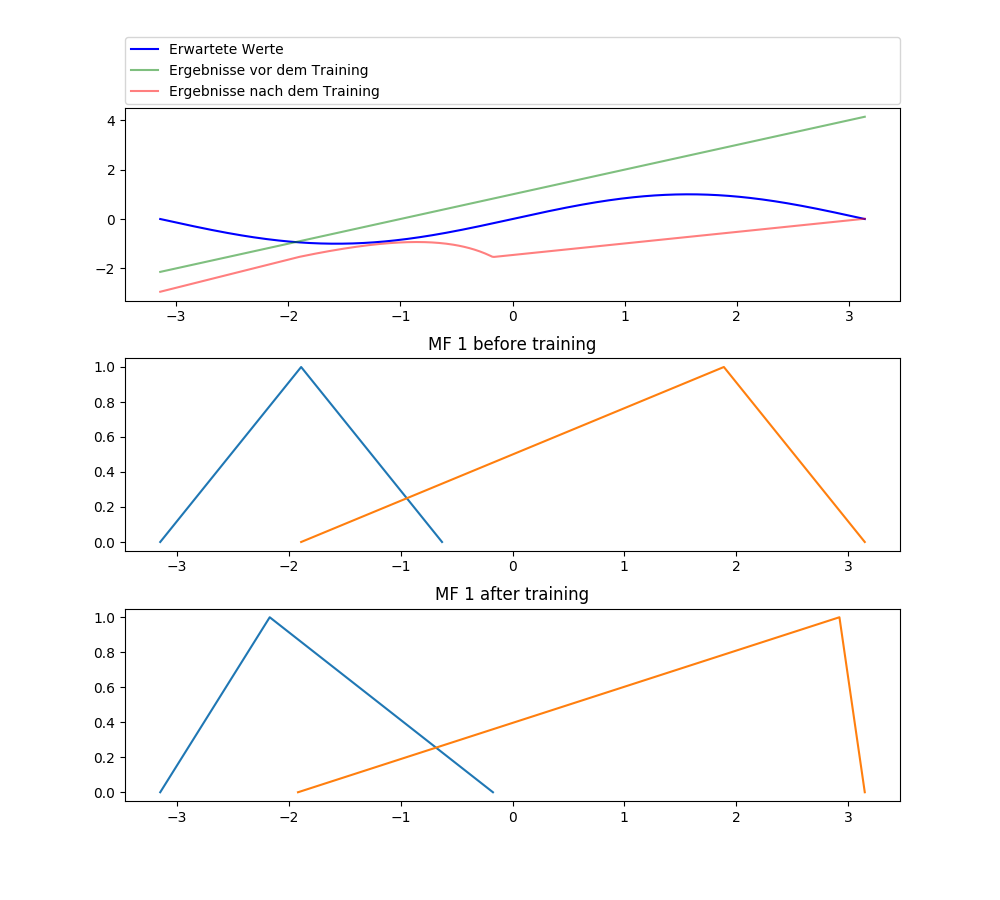
\includegraphics[width=0.65\textwidth]{images/sinus/Stochastic/sinus 1 Input 2 Sets 400 Epochs Stochastic Gradient Descent two equations mf.png}
	\caption{Zwei Fuzzy-Sets, 400 Iterationen, MF-Typ 0} \label{2Sets400_Stoch_0}
\end{figure}



\begin{figure}[htbp]
	\centering
	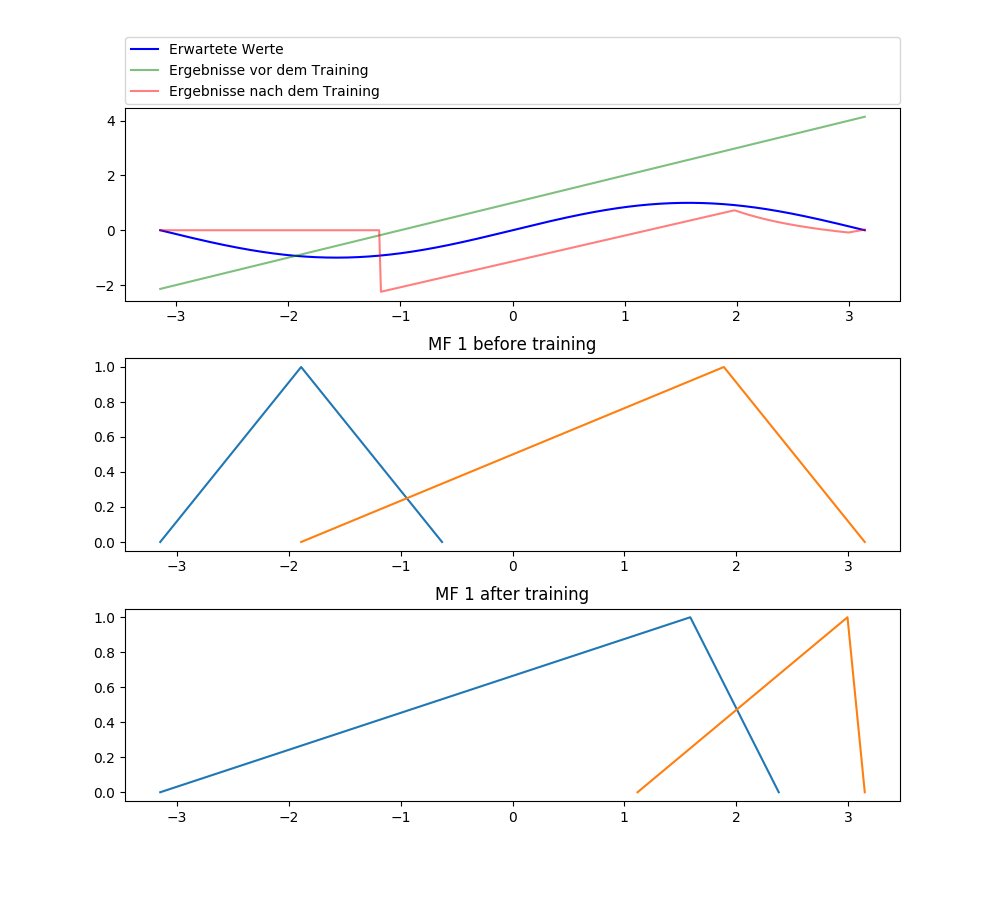
\includegraphics[width=0.65\textwidth]{images/sinus/Stochastic/sinus 1 Input 2 Sets 400 Epochs Stochastic Gradient Descent one equation mf.png}
	\caption{Zwei Fuzzy-Sets, 400 Iterationen, MF-Typ 1} \label{2Sets400_Stoch_1}
\end{figure}

Aus der beiden Abbildungen \ref{2Sets400_Stoch_0} und \ref{2Sets400_Stoch_1} ist es zu bestimmen, dass schon nach einem Lauf große Änderungen zu erkennen sind. In den Abbildungen sind die obersten Grafiken besonders wichtig. Jedoch aus der Abbildung \ref{2Sets400_Stoch_1} ist in der Grafik ein Fehler zu erkennen. Da hat die Funktion im Bereich zwischen -3.2 und -1.2 den 0-Wert. Dieses Fehler scheint weiter in den folgenden Testfällen aufzutauchen, aber verschwindet bei den Mini-Batch- und Batch-Lernverfahren. Interessanterweise erhalten wir zwei unterschiedlichen Endergebnisse, obwohl beide Zugehörigkeitsfunktionen die selbe Funktion berechnen. Man erkennt an den Grafiken weiter, dass die Fuzzy-Sets anders gestalltet sind.

In der Tabelle \ref{tab:2Sets400Epochs} unten ist die Fehlerrate und die Laufzeit abzulesen.

\begin{center}
	\begin{minipage}{\textwidth}
	\begin{tabular}{ | p{3cm} | l | l | p{3cm} | p{3cm} |}
		\hline
		Type & Time & Error & Gradient Type & MF Type \\ \hline
		sinus 1 Input 2 Sets 400 Epochs Stochastic Gradient Descent two equations mf&1.1651129310000004s&1.8500861&Stochastic Gradient Descent&two equations mf
		 \\ \hline
		sinus 1 Input 2 Sets 400 Epochs Stochastic Gradient Descent one equation mf&0.8567342689999995s&0.74594057&Stochastic Gradient Descent&one equation mf
		 \\ \hline
	\end{tabular}
\captionof{table}{Testergebnisse für Modelle mit 2 Fuzzy Sets und 400 Iterationen}\label{tab:2Sets400Epochs}
\end{minipage}
\end{center}

Die interessantesten Spalten aus der Tabelle sind \textit{Time} und \textit{Error}. Die Zahlen deuten, dass MF-Typ 1 die bessere Vorgehensweise sein soll. Jedoch ist das wegen des Fehlers nicht ganz richtig.

Als letztes sind noch die Konklusionsfunktionen der beiden Lernabläufe - Konklusionsfunktionen \ref{mf_0:1} für das Modell mit 2 Sets, 400 Iterationen und MF-Typ 0 und \ref{mf_1:1} für das Modell mit einer Gleichung.

% mf-type 1
%a_0 [[ 0.64128985]
%[-1.45790108]]
%a_y: [[1.14182867]
%[0.46766532]]

% mf-type 2
%a_0 [[-1.14182764]
%[-2.1789615 ]]
%a_y: [[0.94000338]
%[0.35914132]]

\begin{align}
	\begin{split}\label{mf_0:1}
		y_{mft0_1}(x) = 0.64128985 + 1.14182867\cdot x \\
		y_{mft0_2}(x) = -1.45790108 + 0.46766532\cdot x
	\end{split} \\
	\begin{split}\label{mf_1:1}
	y_{mft1_1}(x) = -1.14182764 - 0.94000338\cdot x \\
	y_{mft1_2}(x) = -2.1789615 + 0.35914132\cdot x
	\end{split}	
\end{align}

\subsubsection{Lernen eines Models mit 2 Fuzzy Sets und 10 Abläufe}\label{m2fs10ab}

Der nächste Test endet in 10 Läufe. Die Zwei Tests zeigen keine positiven Ergebnisse. Die Grafiken für die zwei MF-Typen sind sehr Unterschiedlich. Es werden insgesammt vier Tausend Iterationen pro Test durchgeführt, was etwa 7.3s und 6.9s für MF-Typ-0 und MF-Typ-1 entsprechend dauert. Die Abbildungen \ref{2Sets4000_Stoch_0} und \ref{2Sets4000_Stoch_1} stellen die Ergebnisse der Tests dar.

\begin{figure}[htbp]
	\centering
	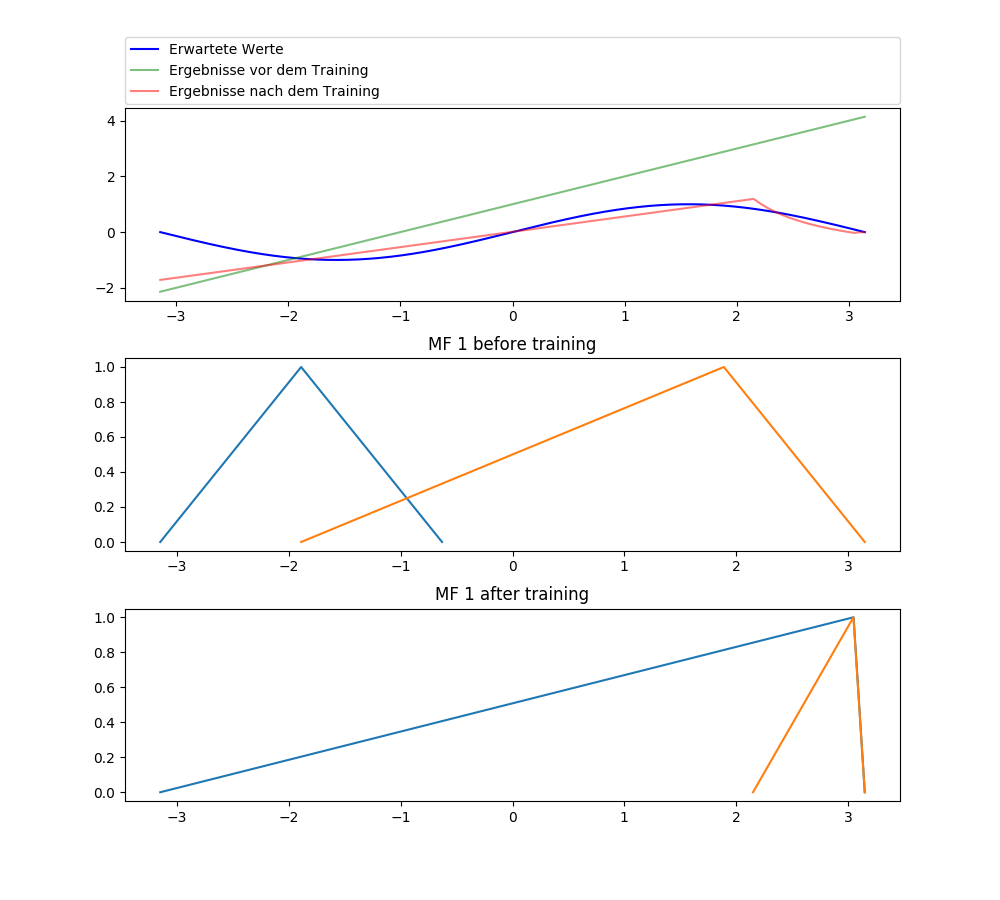
\includegraphics[width=0.65\textwidth]{images/sinus/Stochastic/sinus 1 Input 2 Sets 4000 Epochs Stochastic Gradient Descent two equations mf.png}
	\caption{Zwei Fuzzy-Sets, 4000 Iterationen, MF-Typ 0} \label{2Sets4000_Stoch_0}
\end{figure}
\begin{figure}[htbp]
	\centering
	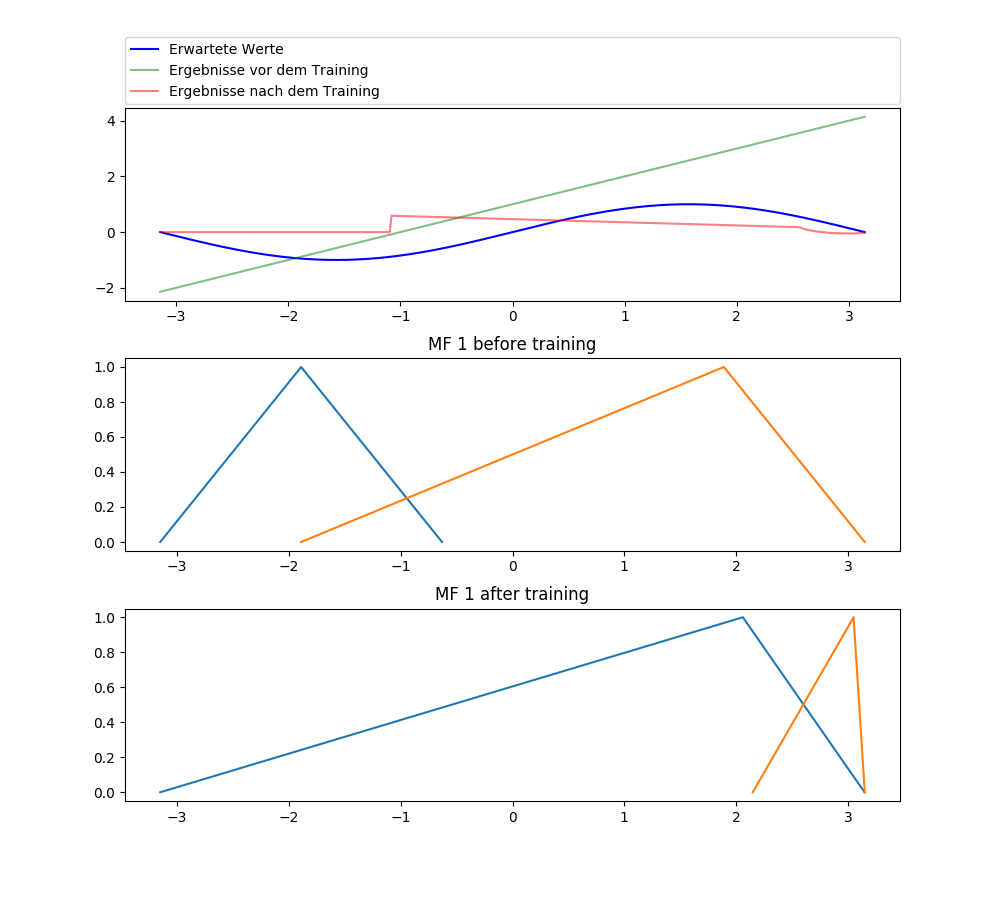
\includegraphics[width=0.65\textwidth]{images/sinus/Stochastic/sinus 1 Input 2 Sets 4000 Epochs Stochastic Gradient Descent one equation mf.png}
	\caption{Zwei Fuzzy-Sets, 4000 Iterationen, MF-Typ 1} \label{2Sets4000_Stoch_1}
\end{figure}

In der Abbildung \ref{2Sets4000_Stoch_1} ist wieder der Fehler in der Berechnung zu bemerken. Der Fehler ergibt sich daraus, dass die Katete der gelbe Zugehörigkeitsfunktion zu lang ist. Was bei kleinen X-Werten dazu führt, dass der rechte Teil der Maximumoperation in der Gleichung \ref{mf_typ1} negativ wird.

Die Konklusionsfunktionen sind für beide Modelle gegeben (\ref{mf_0:10} und \ref{\ref{mf_1:10} sind die Konklusionen entsprechend für die Modelle MF-Typ 0 und MF-Typ 1).
% one equation / MF-Type 0
%a_0 [[ 0.01042824]
%[-1.28822409]]
%a_y: [[ 0.54973926]
%[-0.15157128]]

% one equation / MF-Type 1
%a_0 [[ 0.46553119]
%[-1.52831088]]
%a_y: [[-0.11269253]
%[ 0.44669464]]

\begin{align}
	\begin{split}\label{mf_0:10}
		y_{mft1_1}(x) = 0.01042824 + 0.54973926\cdot x \\
		y_{mft1_2}(x) = -1.28822409 - 0.15157128\cdot x
	\end{split} \\	
	\begin{split}\label{mf_1:10}
		y_{mft2_1}(x) = 0.46553119 - 0.11269253\cdot x \\
		y_{mft2_2}(x) = -1.52831088 + 0.44669464\cdot x
	\end{split}	
\end{align}

Im folgenden Fall gibt es wieder keine Ähnlichkeit zwischen den Konklusionsfunktionen der beiden Modelle.

Die Zeiten und Name als auch die Fehlerrate für beide Modell sind in der Tabelle \ref{tab:2} angegeben. Daraus können zwei Schlüsse gezogen werden.

\begin{center}
	\begin{minipage}{\textwidth}
	\begin{tabular}{ | p{3cm} | l | l | p{3cm} | p{3cm} |}
		\hline
		Type & Time & Error & Gradient Type & MF Type \\ \hline
		sinus 1 Input 2 Sets 4000 Epochs Stochastic Gradient Descent two equations mf&7.308665848s&0.21568511&Stochastic Gradient Descent&two equations mf
		\\ \hline
		sinus 1 Input 2 Sets 4000 Epochs Stochastic Gradient Descent one equation mf&6.9275327529999995s&0.50803167&Stochastic Gradient Descent&one equation mf\\ \hline
	\end{tabular}
\captionof{table}{Testergebnisse für 2 Sets und 4000 Iterationen}\label{tab:2}
\end{minipage}
\end{center}

In der Tabelle können den Fehler und die Laufzeit ausgelesen werden. Anhand der Daten aus dieser Tabelle lässt sich sagen, dass die Berechnung für Modelle des Typs MF-1 kürzer ist, aber das Typ 0 Modell besser lernt.

\subsubsection{Lernen eines Models mit 8 Fuzzy Sets und 10 Abläufe}\label{m8fs10ab}
Im folgenden Testfall ist zu untersuchen, wie die Laufzeit beieinflußt wird, wenn sich die Anzahl der Fuzzymengen erhöht. Im Folgenden Unterkapitel wird der Test mit \textbf{8} Fuzzy-Sets ausgeführt.

Die Ergebnissgrafiken sind zunächst gegeben (\ref{8Sets4000_Stoch_0} und \ref{8Sets4000_Stoch_1}).

\begin{figure}[htbp]
	\centering
	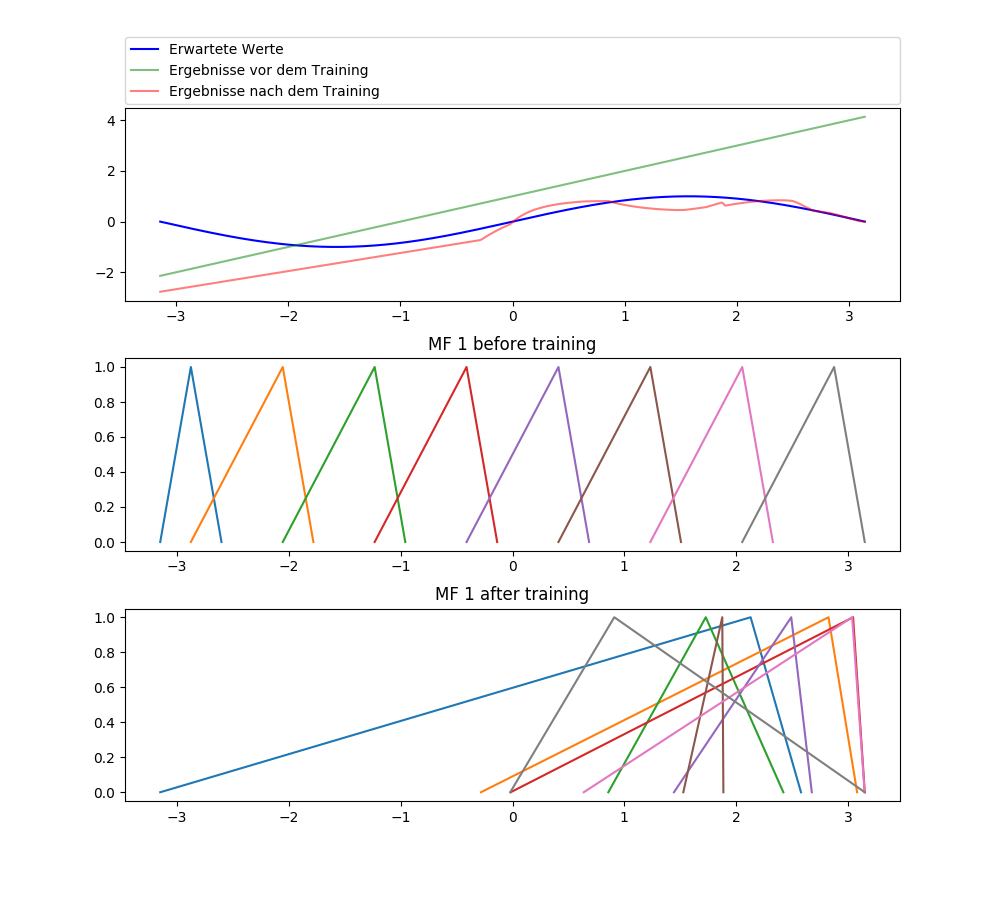
\includegraphics[width=0.65\textwidth]{images/sinus/Stochastic/sinus 1 Input 8 Sets 4000 Epochs Stochastic Gradient Descent two equations mf.png}
	\caption{Acht Fuzzy-Sets, 4000 Iterationen, MF-Typ 0} \label{8Sets4000_Stoch_0}
\end{figure}
\begin{figure}[htbp]
	\centering
	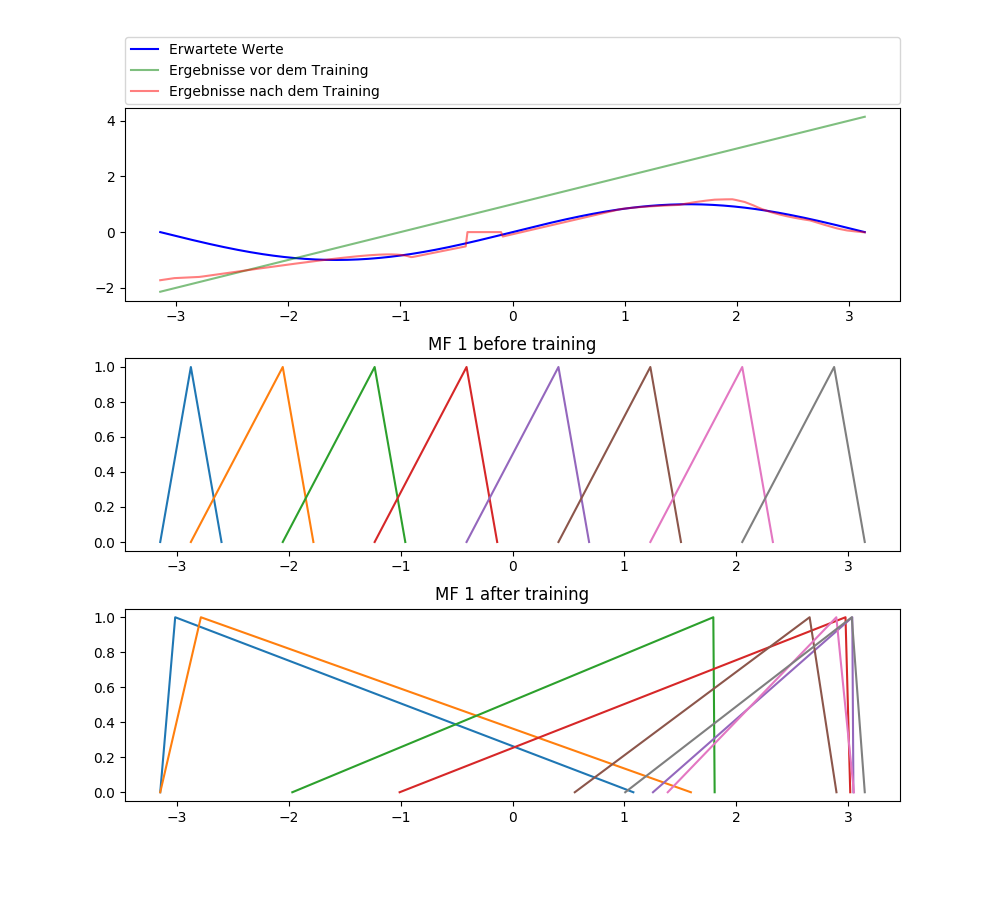
\includegraphics[width=0.65\textwidth]{images/sinus/Stochastic/sinus 1 Input 8 Sets 4000 Epochs Stochastic Gradient Descent one equation mf.png}
	\caption{Acht Fuzzy-Sets, 4000 Iterationen, MF-Typ 1} \label{8Sets4000_Stoch_1}
\end{figure}

An den Abbildugen erkennt man, dass sich die Funktion mit mehr Fuzzy-Mengen besser lernen lässt. Man sieht auch große Unterschiede in der Art der gelernten Fuzzymengen. Es ist zu bemerken, dass alle ab dem zweiten Fuzzyset in der ersten Abbildung in die zweite Hälfte des Wertebereichs vollgestopft werden. Während in der zweite Abbildung ab dem dritten Fuzzyset. Das ist nur deswegen geschehen, weil bei dem Lernen immer Einzelelemente aus der Datenmenge gezogen werden. Üblicherweise werden beim Lernen immer die betroffenen Parametern nach jeder Iteration angepasst. Also die erste Menge wird als erstes angesprochen und angepasst. Da der linke Parameter nicht geändert werden kann, bedeutet das, dass nur der Mittel- und rechten Grenzparameter nach rechts geschoben werden. Dies erklärt die Vollstopfung am rechten Rand des Wertebereichs.

Die Ergebnisse sind in Tabelle \ref{tab8_4000St} abzulesen.

\begin{center}
	\begin{minipage}{\textwidth}
	\begin{tabular}{ | p{3cm} | l | l | p{3cm} | p{3cm} |}
		\hline
		Type & Time & Error & Gradient Type & MF Type \\ \hline
		sinus 1 Input 8 Sets 4000 Epochs Stochastic Gradient Descent two equations mf&17.413568215999998&0.80348945&Stochastic Gradient Descent&two equations mf \\ \hline
		sinus 1 Input 8 Sets 4000 Epochs Stochastic Gradient Descent one equation mf&14.525632421000001&0.21442673&Stochastic Gradient Descent&one equation mf\\ \hline
	\end{tabular}
\captionof{table}{Testergebnisse für 8 Fuzzy-Sets und 4000 Iterationen}\label{tab8_4000St}
\end{minipage}
\end{center}

Aus der Tabelle lässt sich herauslesen, dass der zweite Test (siehe \ref{8Sets4000_Stoch_1}) deutlich schneller und akkurater lernt. Auf der Abbildung \ref{8Sets4000_Stoch_1} ist eine Stuffe im Mittleren Bereich zu erkennen, wo sich der Fehler zeigt. Es ist zu lesen, dass das Typ 1 \textit{3} Sekunden schneller ist. Man sieht auch, dass das Verfahren deutlich näher an dem Sollfunktion ist als Typ 0.

Ich gebe die Konklusionsfunktionen für MF-Typ 0 \ref{8mf_0:10} und MF-Typ 1 \ref{8mf_1:10} nur informative an. Daran können keine weitere Rückschlüsse genannt werden. 
% MF-Typ 0
%a_0 [[-0.5235794 ]
%[ 2.93676464]
%[-3.65265173]
%[ 2.85619127]
%[ 0.1644323 ]
%[-0.92605422]
%[ 0.26038533]
%[ 0.63168423]]
%a_y: [[ 0.71489089]
%[-0.78074253]
%[ 1.63942728]
%[-0.87280814]
%[ 0.55701768]
%[ 1.26660038]
%[-0.12738553]
%[-0.15357252]]
\begin{align}
\begin{split}\label{8mf_0:10}
y_{mft1_1}(x) = -0.5235794 + 0.71489089\cdot x \\
y_{mft1_2}(x) = 2.93676464 - 0.78074253\cdot x \\
y_{mft1_3}(x) = -3.65265173 + 1.63942728\cdot x \\
y_{mft1_4}(x) = 2.85619127 - 0.87280814\cdot x \\
y_{mft1_5}(x) = 0.1644323 + 0.55701768\cdot x \\
y_{mft1_6}(x) = -0.92605422 + 1.26660038\cdot x \\
y_{mft1_7}(x) = 0.26038533 - 0.12738553\cdot x \\
y_{mft1_8}(x) = 0.63168423 - 0.15357252\cdot x
\end{split} \\
% MF-Typ 1
%a_0 [[ 0.46676819]
%[-0.17691342]
%[-0.07739224]
%[ 1.28046489]
%[-1.72202347]
%[ 1.398913  ]
%[ 0.06231506]
%[-0.04088159]]
%a_y: [[ 0.41699012]
%[ 0.80520989]
%[ 0.93785577]
%[-0.94272644]
%[ 0.71823673]
%[ 0.30636544]
%[-0.17987376]
%[-0.28006114]]
\begin{split}\label{8mf_1:10}
y_{mft1_1}(x) = 0.46676819 + 0.41699012\cdot x \\
y_{mft1_2}(x) = -0.17691342 + 0.80520989\cdot x \\
y_{mft1_3}(x) = -0.07739224 + 0.93785577\cdot x \\
y_{mft1_4}(x) = 1.28046489 - 0.94272644\cdot x \\
y_{mft1_5}(x) = -1.72202347 + 0.71823673\cdot x \\
y_{mft1_6}(x) = 1.398913 + 0.30636544\cdot x \\
y_{mft1_7}(x) = 0.06231506 - 0.17987376\cdot x \\
y_{mft1_8}(x) = -0.04088159 - 0.28006114\cdot x
\end{split}	
\end{align}

\subsection{Schlussfolgerung}
Hier ist schwehr die beste Konfiguration fürs Lernen zu nennen. Ich würde sogar sagen, dass das Lernen mit dem stochastischen Verfahren ungeeignet ist. Im nächsten Kapitel wird das Mini-Batch-Verfahren ausgetestet.

Aus den Zahlreichen Tests, die durchgeführt worde, wurde beschlossen, dass MF-Typ 1 Modelle nicht geeignet ist, da auch asymmetrische Fuzzy-Mengen zugelassen sind die MF-Typ 1 Berechnung nicht dafür geeignet ist. 
%\begin{tabular}
%	
%\end{tabular}
\section{Lernen der Sinusfunktion mit Mini-Batch Gradient Descent}\label{lernen_mb}

In diesem Kapitel handelt es sich um die Mini-Batch Gradient Descent Verfahren. Das Verfahren wurde am Anfang dieses \ref{mini_batch}. Kapitels vorgestellt. Ziel der folgenden Untersuchungen ist es zu zeigen, welche die beste Konfiguration fürs Model ist. Außerdem werden im Fazit die beiden Verfahren (Mini-Batch und Stochastic) verglichen. 

\subsubsection{Lernen der Sinusfunktion mit 2 Fuzzy-Sets und 1 Ablauf}

Begonnen werden soll mit dem Lernen der Funktion mit zwei Fuzzymengen und der Ablauf verläuft über einen Gang. Die Testbeschreibung beinhaltet nur den MF-Typ 0.

\begin{figure}[htbp]
	\centering
	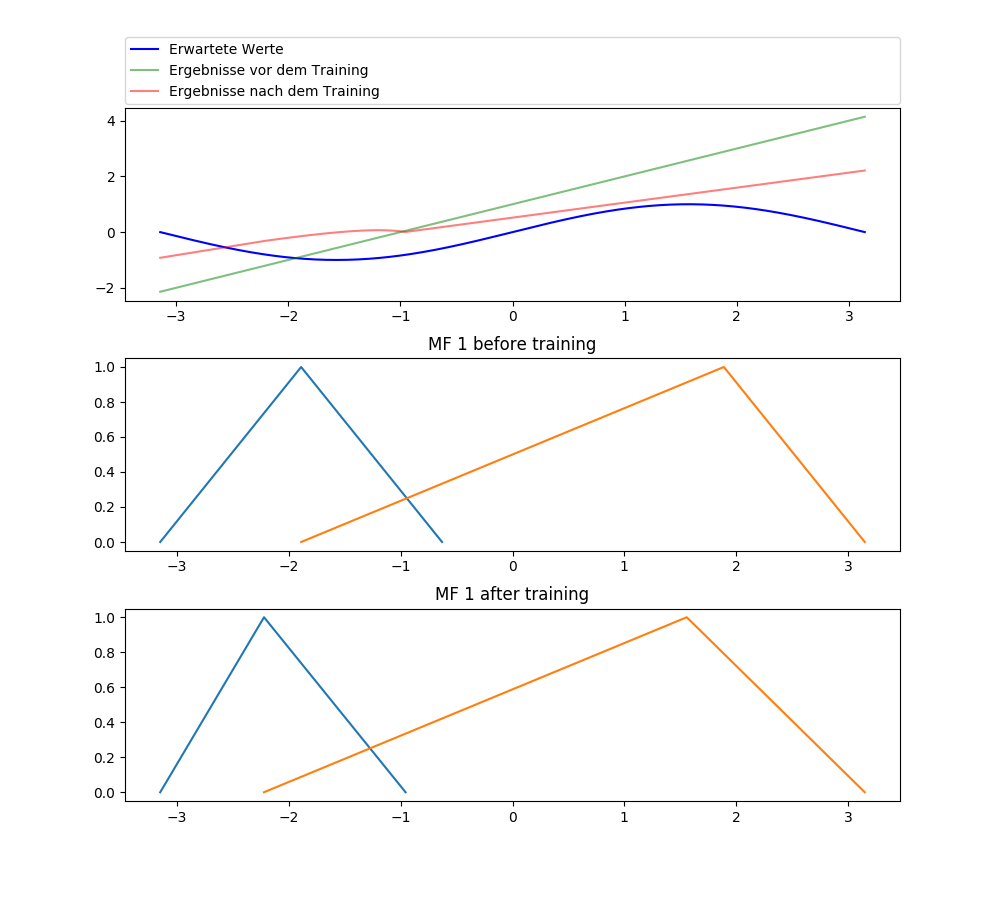
\includegraphics[width=0.75\textwidth]{images/sinus/Mini-Batch/sinus 1 Input 2 Sets 5 Epochs Mini-Batch Gradient Descent two equations mf.png}
	\caption{2 Fuzzy-Sets, 5 Iterationen, MF-Typ 0} \label{2mini_batch5:0}
\end{figure}

In der Abbildung \ref{2mini_batch5:0} sieht man keine große Änderung in den Fuzzy-Sets als auch in der Ergebnissfunktion. Das ist jedoch kein Wunder, da es nur 5 Iterationen durchgeführt werden. Die Dauer dieses Tests entspricht 14 ms.

Zur Abgleich habe ich die Ergebnisse aus dem vorrigen Unterkapitel und diesem Test in der Tabelle \ref{tab2_5MB} angegben.
\begin{center}
	\begin{minipage}{\textwidth}
	\begin{tabular}{ | p{3cm} | l | l | p{3cm} | p{3cm} |}
		\hline
		Type & Time & Error & Gradient Type & MF Type \\ \hline
		sinus 1 Input 2 Sets 5 Epochs Mini-Batch Gradient Descent two equations mf&0.1438041160000001&0.70317644&Mini-Batch Gradient Descent&two equations mf \\ \hline
		sinus 1 Input 2 Sets 400 Epochs Stochastic Gradient Descent two equations mf&1.1651129310000004s&1.8500861&Stochastic Gradient Descent&two equations mf
		\\ \hline
	\end{tabular} 
\captionof{table}{Testergebnisse für Mini-Batch und Stochastic}\label{tab2_5MB}
\end{minipage}
\end{center}

Die Fehlerrate ist wie erwartet sehr hoch, jedoch viel kleiner als der von Stochastischen Verfahren. Außerdem ist die Endfunktion sehr ähnlich wie aus der Vorrigenkapitel (siehe \ref{2Sets400_Stoch_0}). Man erkennt aus den beiden Abbildungen, dass in Abbildung \ref{2Sets400_Stoch_0} die Funktion im Negativen Y-Bereich liegt.%, während die \ref{2mini_batch5:0} nur in dem Abschnit zwischen -3.2 bis ungefähr -1. 

Es ist eine schnellere Laufzeit als der stochastische Verfahren zu erkennen. Die kürze Lerndauer erklärt sich dadurch, da der Datensatz schneller abgearbeitet wird - in Fünf Schritte, im Vergleich zu Vierhundert. Es ist zu erwarten, dass nach 400 Iterationen das Modell noch besser (niedrigere Fehlerrate zu erweisen) sein soll. Im nächsten Kapitel wird diese Aussage untersucht.

Schließlich gebe ich die Konklusionsfunktionen für das Model in \ref{2mini_mf_0:0}.

%MF-Typ 0
%a_0 [[1.12589365]
%[0.51933658]]
%a_y: [[0.65193717]
%[0.53854825]]

\begin{align}
\begin{split}\label{2mini_mf_0:0}
y_{mft1_1}(x) = 1.12589365 + 0.65193717\cdot x \\
y_{mft1_2}(x) = 0.51933658 + 0.53854825\cdot x
\end{split}
\end{align}

Zwischen die Funktionen \ref{2mini_mf_0:0} und \ref{mf_0:1} ist in die Erste Gleichung zu erkennen, dass sich die Parametern ihren Platz getauscht haben. Ein weiterer Unterschied ist, dass es keine negativen Parametern gelernt wurden.

%MF-Typ 1
%a_0 [[0.95071704]
%[0.51425419]]
%a_y: [[0.70936966]
%[0.52004189]]

\subsubsection{Lernen der Sinusfunktion mit 2 Fuzzy-Sets und 10 Ablauf}
Als nächstes ist das Model mit 10 Abläufe zu betrachten. Die Frage, die in diesem Kapitel beantwortet werden soll, ist, ob das Lernen mit einem Bruchteil der Datenmenge wirklich besser ist. Deswegen vergleiche ich die Ergebnisse von Kapitel \ref{m2fs10ab} mit den aus diesem. 

Eine Ergebnissabbildung wird in \ref{2mini_batch50:0} gezeichnet.

\begin{figure}[htbp]
	\centering
	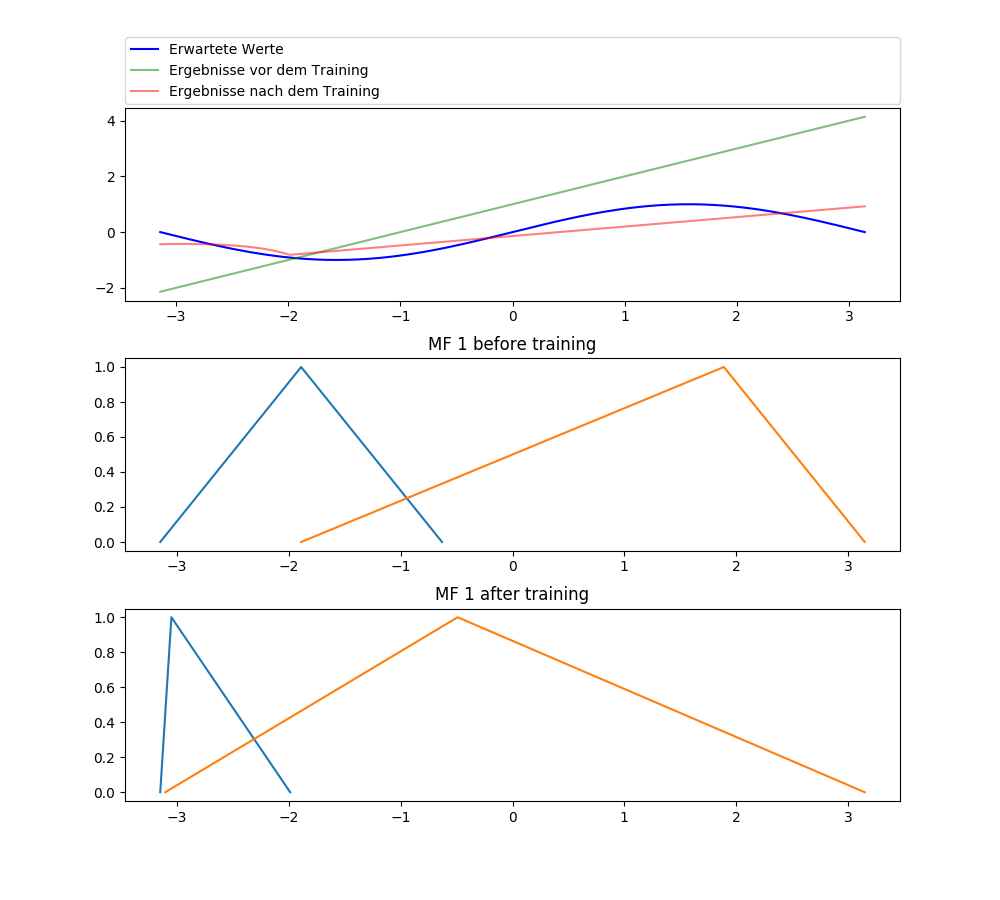
\includegraphics[width=0.65\textwidth]{images/sinus/Mini-Batch/sinus 1 Input 2 Sets 50 Epochs Mini-Batch Gradient Descent two equations mf.png}
	\caption{2 Fuzzy-Sets, 50 Iterationen, MF-Typ 0} \label{2mini_batch50:0}
\end{figure}

Die Fuzzy-Mengen haben eine deutlich größere Änderung im Vergleich zu dem aus vorrigen Kapitel Modell unterlegen. Das Lernen hat 0.2s gedauert. Das ist etwa 30 Mal schneller als der stochastische Verfahren. Die Daten für beide Modelle stehen mit Fehlerrate und Dauer in der Tabelle \ref{tab2_50MB}.

\begin{center}
	\begin{minipage}{\textwidth}
	\begin{tabular}{ | p{3cm} | l | l | p{3cm} | p{3cm} |}
		\hline
		Type & Time & Error & Gradient Type & MF Type \\ \hline
		sinus 1 Input 2 Sets 50 Epochs Mini-Batch Gradient Descent two equations mf&0.2727800499999997&0.1554767&Mini-Batch Gradient Descent&two equations mf\\ \hline
		sinus 1 Input 2 Sets 4000 Epochs Stochastic Gradient Descent two equations mf&7.308665848s&0.21568511&Stochastic Gradient Descent&two equations mf
		\\ \hline
	\end{tabular}  
\captionof{table}{Erbenisvergleich zwischen dem Mini-Batch- und Stochastic-Modell}\label{tab2_50MB}

\end{minipage}
\end{center}

Man erzielt nicht nur ein schnelleres Lernen mit dem Mini-Batch Verfahren,sondern auch ein besseres. Die Fehlerrate ist von 0.22 um etwa 30\% auf 0.16 abgestiegen.

Zum Schluss sind die Inferenzfunktionen \ref{conc_50MB} für das Modell gegeben.

% mftyp 0
%a_0 [[ 0.58986986]
%[-0.14078197]]
%a_y: [[0.32787314]
%[0.3395195 ]]

\begin{align}
\begin{split}\label{conc_50MB}
	y_{mft1_1}(x) = 0.58986986 + 0.32787314\cdot x \\
	y_{mft1_2}(x) = -0.14078197 + 0.3395195\cdot x
\end{split}
\end{align}

\subsubsection{Lernen der Sinusfunktion mit 2 Fuzzy-Sets und 1000 Abläufe}\label{sinus_mb_2_1000}
In diesem Abschnitt wird das Ergebnis aus dem Test mit 1000 Abläufe vorgestellt. Das Model verfügt weiterhin über 2 Fuzzymengen und wird mit MF-Typ 0 gelernt. %Die Abbildung \ref{2mini_batch1000:0} berichtet das Endergebniss.

Bei dieser Konfiguration lernt das Model mit nur einer Zugehörigkeitsgleichung auch sehr erfolgreich. Die Abbildungen der beiden Tests sind sehr ähnlich. Die Abbildungen \ref{2mini_batch1000:1} und \ref{2mini_batch1000:0} berichten das Ergebnis.

\begin{figure}[htbp]
	\centering
	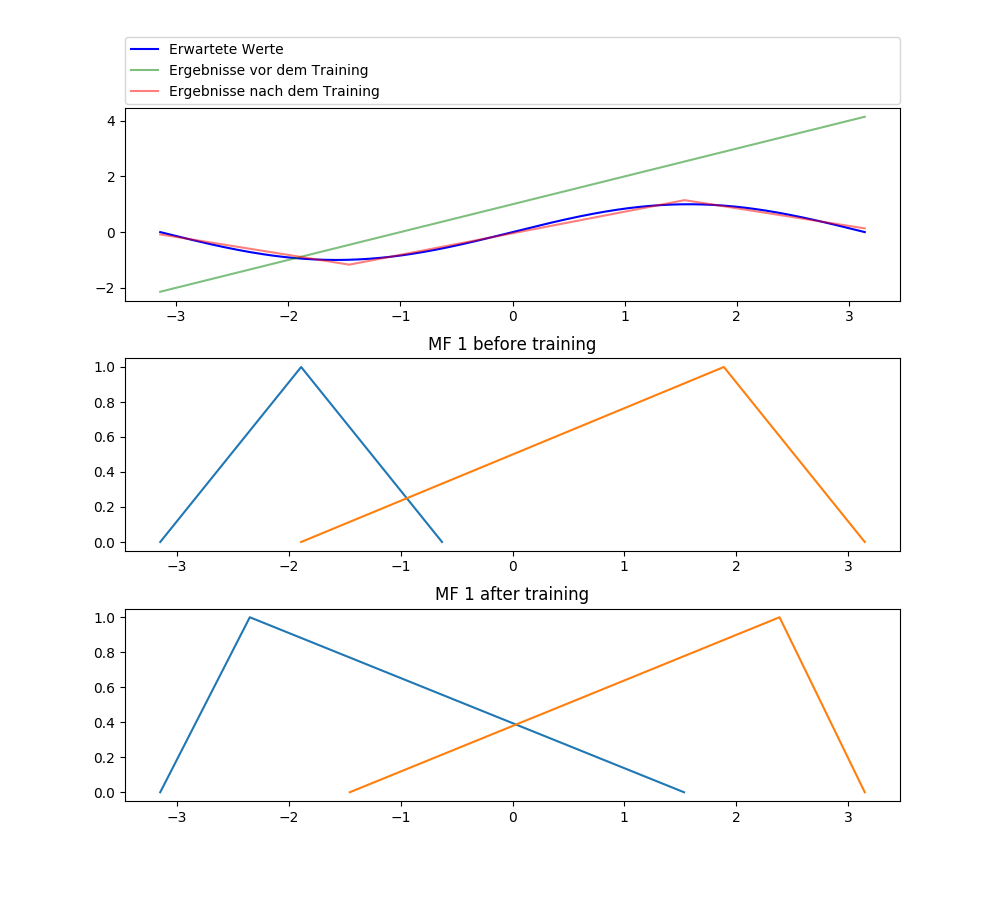
\includegraphics[width=0.65\textwidth]{images/sinus/Mini-Batch/sinus 1 Input 2 Sets 5000 Epochs Mini-Batch Gradient Descent two equations mf.png}
	\caption{2 Fuzzy-Sets, 1000 Iterationen, MF-Typ 0} \label{2mini_batch1000:0}
\end{figure}
\begin{figure}[htbp]
	\centering
	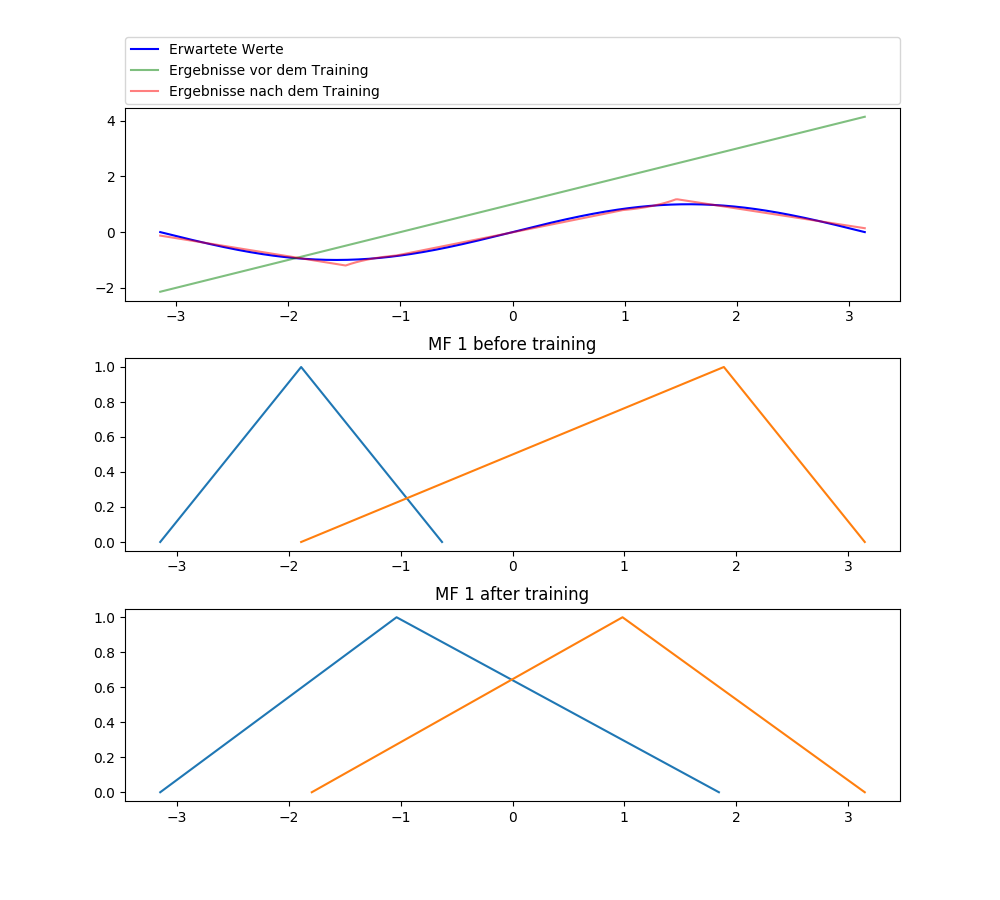
\includegraphics[width=0.65\textwidth]{images/sinus/Mini-Batch/sinus 1 Input 2 Sets 5000 Epochs Mini-Batch Gradient Descent one equation mf.png}
	\caption{2 Fuzzy-Sets, 1000 Iterationen, MF-Typ 0} \label{2mini_batch1000:1}
\end{figure}

Das Endergebnis aus der Abbildung \ref{2mini_batch1000:1} scheint auf den ersten Blick besser zu sein. Der größte Unterschied liegt in den Fuzzymengen. Die gelernten Fuzzysets überlappen zur unterschiedlichen Stuffen. Die Mengen in der Abbildung \ref{2mini_batch1000:1} überschneiden sich deutlich mehr. Die Reichweite ist in der Abbildung \ref{2mini_batch1000:1} etwa 3 cm und auf der Abbildung \ref{2mini_batch1000:0} sind es ungefähr 2. Die zusätzlichen Daten, die in der Tabelle \ref{tab2_1000MB} zu finden sind, beantworten die Frage, welches Model besser ist.

\begin{center}
	\begin{minipage}{\textwidth}
	\begin{tabular}{ | p{3cm} | l | l | p{3cm} | p{3cm} |}
		\hline
		Type & Time & Error & Gradient Type & MF Type \\ \hline
		sinus 1 Input 2 Sets 5000 Epochs Mini-Batch Gradient Descent two equations mf&11.761141329s&0.006521431&Mini-Batch Gradient Descent&two equations mf \\ \hline
		sinus 1 Input 2 Sets 5000 Epochs Mini-Batch Gradient Descent one equation mf&10.697818779s&0.0048954873&Mini-Batch Gradient Descent&one equation mf \\ \hline 
	\end{tabular}
\captionof{table}{Testergebnisse für Modelle mit 2 Sets und 5000 Iterationen}\label{tab2_1000MB}
\end{minipage}
\end{center}

Die Vermutung war richtig. Das zweite Model ist mit etwa 0,02 Einheiten besser und mit einer Sekunde schneller. Die Frage taucht jetzt auf, wo liegt der Unterschied zwischen die beiden Modellen? Ist es wegen des Unterschieds in der Fuzzymengen, oder sind die Inferenzfunktionen einfach unterschiedlich? Die Antwort wird erst klar, wenn die Gleichungen für die Konklusionen betrachtet werden. Analog gehören die ersten beiden Gleichung in \ref{2mf_0:1000} dem Modell mit zwei Gleichungen (MF-Typ 0) und entsprechend \ref{2mf_1:1000} dem Modell mit einer Gleichung (MF-Typ 1).



% Endfunktion mftyp 0
%a_0 [[-2.10781751]
%[ 2.1163349 ]]
%a_y: [[-0.64453965]
%[-0.63109723]]

% Endfunktion mftyp 1
%a_0 [[-2.17036302]
%[ 2.09081218]]
%a_y: [[-0.65073889]
%[-0.62095912]]

\begin{align}
\begin{split}\label{2mf_0:1000}
y_{mft1_1}(x) = -2.10781751 - 0.64453965\cdot x \\
y_{mft1_2}(x) = 2.1163349 - 0.63109723\cdot x
\end{split} \\	
\begin{split}\label{2mf_1:1000}
y_{mft2_1}(x) = -2.17036302 - 0.65073889\cdot x \\
y_{mft2_2}(x) = 2.09081218 - 0.62095912\cdot x
\end{split}	
\end{align}

Die Antwort auf die Frage lautet, dass der Unterschied liegt in den Fuzzymengen. Die Gleichungen sind bis auf der zweiten Dezimalzahl identisch. Die Tatsache, dass die Werte überhaupt so ähnlich sind, ist ein Wunder.

Wenn man die Ergebnisse aus Unterkapitel \ref{lernen_mb} betrachtet, erkennt man wie schlecht das stochastische Verfahren lernt. Allein mit \textbf{10} Abläufe (4000 Iterationsschritte) bei dem Stochastischen-Test (siehe Tabelle \ref{tab:2}) hat man fast die selbe Anzahl an Iterationsschritten (5000) bei dem Mini-Batch-Test (siehe \ref{tab2_1000MB}) und trotzdem ist das Ergebniss \textbf{100} mal schlechter.

\section{Lernen der Sinusfunktion mit Batch Gradient Descent}
Weiterhin werden Modelle erstellt, die das Batch Gradient Descent Verfahren benutzen, um die Sinusfunktion zu erlernen. Jedes Testmodell wird 1000 Abläufe, oder 1000 Iterationen (siehe \ref{batch}), laufen gelassen, aber jedes unterscheidet sich vom nächsten in der Anzahl der Fuzzy-Mengen. Es werden zwei Tests durchgeführt, um zu bestimmen, welche ist die optimale, bzw. ausreichende, Anzahl an Fuzzy-Mengen. Die drei Tests werden entsprechen mit 2 und 3 Fuzzy-Sets trainiert. Außerdem es wird einen Vergleich mit Mini-Batch gezogen. Es ist interessant zu prüfen, ob die beiden Verfahren auch unterschiedliche Ergebnisse erzielen würden.

\subsection{Lernen mit 2 Fuzzy-Sets}\label{lernene_2S_b}
Das erste Testmodelle wird mit 2 Fuzzy-Mengen initialisiert und der Test wird 1000 Abläufe durchgeführt. Das Ergebnis wird in der Abbildung \ref{batch_2_1000} und in der Tabelle \ref{table_2_1000} beschrieben.

\begin{figure}[htbp]
	\centering
	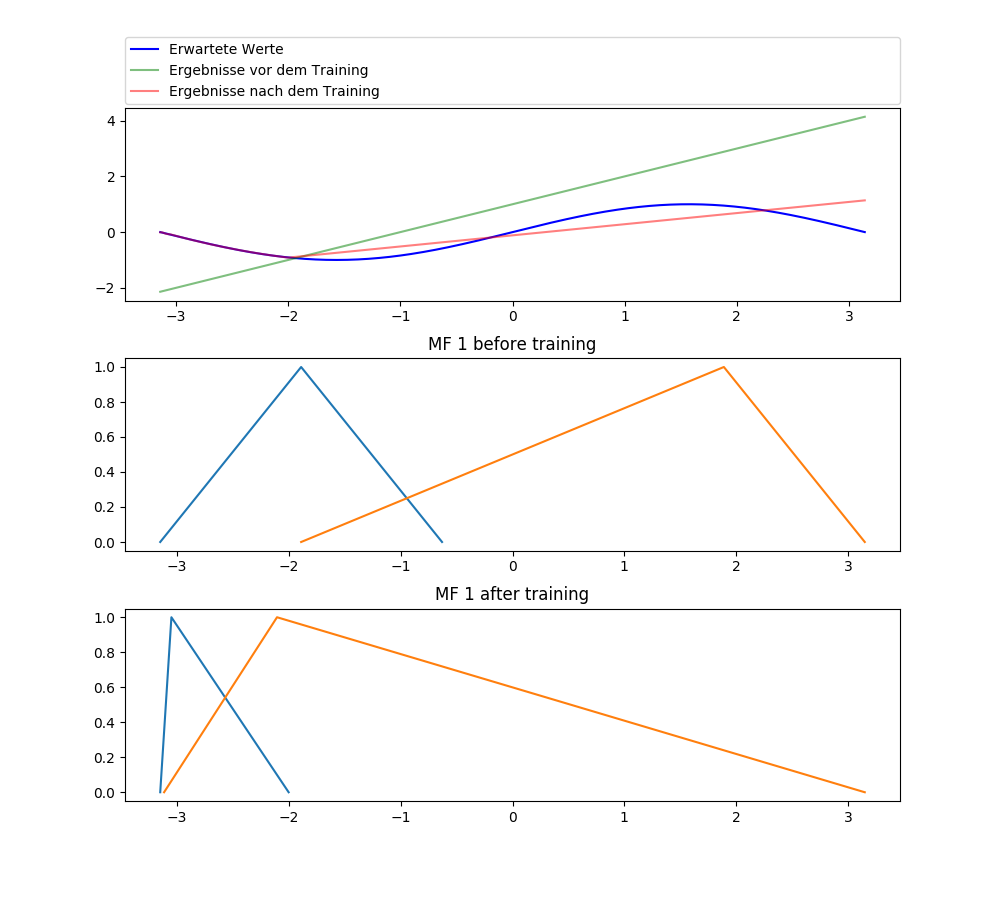
\includegraphics[width=0.65\textwidth]{images/sinus/Batch/sinus 1 Input 2 Sets 1000 Epochs Batch Gradient Descent two equations mf.png}
	\caption{Batch Modell mit 2 Fuzzy-Sets, 1000 Iterationen und MF-Typ 0} \label{batch_2_1000}
\end{figure}

Der Abbildung \ref{batch_2_1000} nach wird in dem Anfangsbereich zwischen den X-Werteb -3.2 und -2.0 scheint die Kurve gut angepasst zu werden. Im späteren Bereich (-2.0 bis 3.2) ist keine Kurve mehr, sondern eine Gerade. Das liegt daran, dass die Fuzzymengen nur zum kleinen Teil überlappen, zwar nur zwischen -3.2 und 2.0, darum auch die anliegende Kurve. Wenn dieses Ergebniss mit dem aus letzen Unterkapitel (siehe \ref{sinus_mb_2_1000}) verglichen wird, sieht man den Unterschied in den Fuzzymengen. Hier schon erkennt man, dass das Mini-Batch-Verfahren geeigneter ist als das Batch. Die Begründung dafür ist, dass mit dem Mini-Batch-Verfahren nach 1000 Abläufe ein gut tranierter Modell erhalten wird. Die Tabelle verschafft uns weitere Information darüber, wie gut das Modell ist.
%


\begin{center}
	\begin{minipage}{\textwidth}
	\begin{tabular}{ | p{3cm} | l | l | p{3cm} | p{3cm} |}
		\hline
		Type & Time & Error & Gradient Type & MF Type \\ \hline
		sinus 1 Input 2 Sets 1000 Epochs Batch Gradient Descent two equations mf&2.1207925870000004&0.13913395&Batch Gradient Descent&two equations mf \\ \hline
		sinus 1 Input 2 Sets 5000 Epochs Mini-Batch Gradient Descent two equations mf&11.761141329s&0.006521431&Mini-Batch Gradient Descent&two equations mf \\ \hline
	\end{tabular}
\captionof{table}{Testergebnisse für die Modelle mit Batch- und Mini-Batch-Verfahren}\label{table_2_1000}
\end{minipage}
\end{center}

Wenn die Zeilen aus der Tabelle \ref{table_2_1000} verglichen wird, erkennt man, dass das Mini-Batch Verfahren besser ist. In der Tabelle kann man lesen, dass es zwei unterschiedliche Werte für die Iterationen der Modelle figurieren. Dies entsteht aus den Unterschieden in der beiden Verfahren (Mini-Batch und Batch). In beiden Testfällen wird 1000 Abläufe durchgeführt, was bei dem Mini-Batch-Modell 5000 Iterationen sind, da einen Ablauf aus fünf Iterationen besteht. Daraus ergibt sich eine natürliche Verzögerung in der Berechnung(dem Lernen). Was aber nicht bestreiten kann ist die Fehlerrate. Hier erweist das Mini-Batch-Modell eine Verbesserung um zwei Stellen nach der Komma.

\subsection{Lernen mit 3 Fuzzy-Sets}
In dieser Unterkapitel wird ein Test mit 3 Fuzzy-Mengen durchgeführt. Das Modell besitzt die selben Eigenschaften wie das aus dem letzen Unterkapitel(siehe \ref{lernene_2S_b}). Analog zur Unterkapitel \ref{lernene_2S_b} wird zuerst eine Abbildung und danach eine Tabelle analysier, jedoch wird jetzt einen Vergleich zwischen dem Modell aus \ref{batch_2_1000} und dem Modell in der Abbildung \ref{batch_3_1000} gezogen. Ziel hier ist es zu prüfen, ob eine Erhöhung der Fuzzy-Sets zum besseren Ergebniss führt. Die Abbildung \ref{batch_3_1000} zeigt das Endergebniss.

\begin{figure}[htbp]
	\centering
	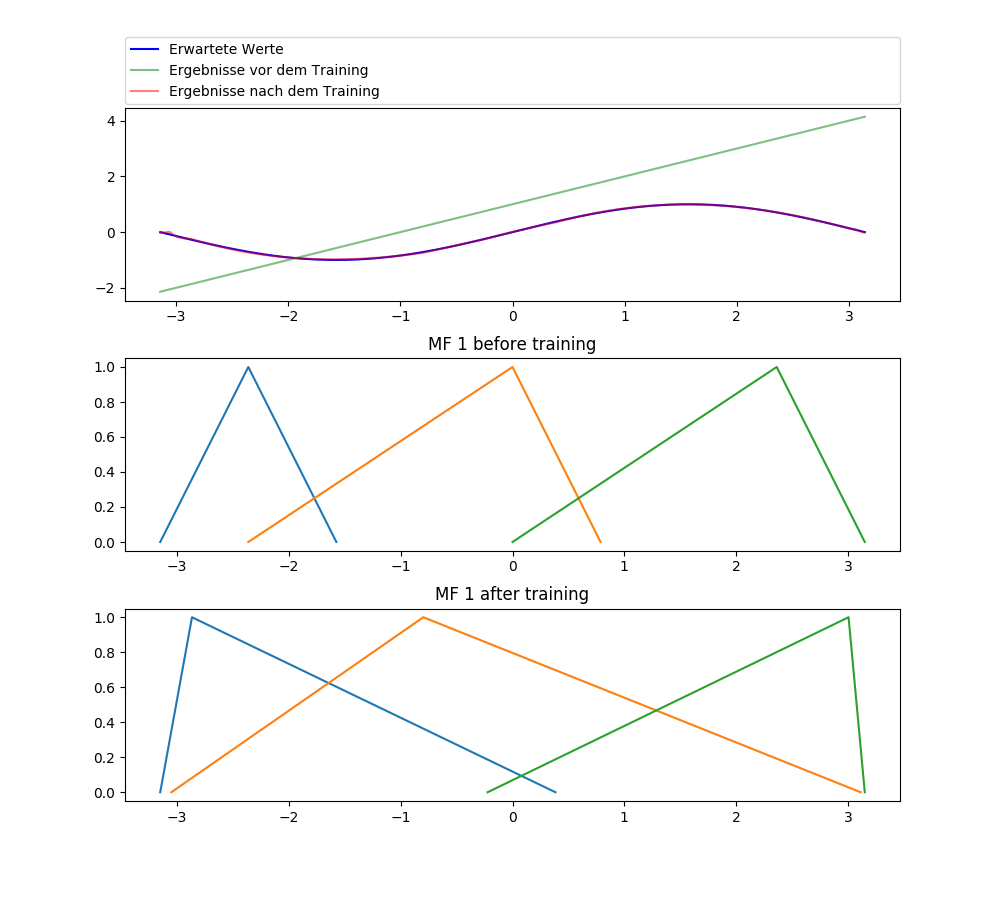
\includegraphics[width=0.65\textwidth]{images/sinus/Batch/sinus 1 Input 3 Sets 1000 Epochs Batch Gradient Descent two equations mf.png}
	\caption{Batch Modell mit 3 Fuzzy-Sets, 1000 Iterationen und MF-Typ 0} \label{batch_3_1000}
\end{figure}

Die Abbildung \ref{batch_3_1000} zeigt eine deutliche Verbesserung in dem, wie die Sinusfunktion gelernt wird. Es kann sogar gesagt werden, dass die Funktion sehr gut gelernt ist. Hier ist es wichtig darauf zu weisen, dass alle drei Fuzzy Mengen zu einem gewissen Teil überlappen. Daraus entsteht auch die fast perfekte Kurve, die die gesuchte Funktion überdeckt.
Weiterhin wird die Tabelle \ref{table_3_1000} untersucht

\begin{center}
	\begin{minipage}{\textwidth}
	\begin{tabular}{ | p{3cm} | l | l | p{3cm} | p{3cm} |}
		\hline
		Type & Time & Error & Gradient Type & MF Type \\ \hline
		sinus 1 Input 2 Sets 1000 Epochs&2.1207925870000004&0.13913395&Batch Gradient Descent&two equations mf \\ \hline
		sinus 1 Input 3 Sets 1000 Epochs&2.528284161&0.00021747834&Batch Gradient Descent&two equations mf
		\\ \hline
		sinus 1 Input 2 Sets 5000 Epochs&11.761141329s&0.006521431&Mini-Batch Gradient Descent&two equations mf \\ \hline
		sinus 1 Input 3 Sets 5000 Epochs&12.479160914&0.00017558844&Mini-Batch Gradient Descent&two equations mf\\ \hline	
	\end{tabular}
	\captionof{table}{Testergebnisse für die Modelle mit zwei und drei Fuzzy-Mengen und Mini-Batch- und Batch-Verfahren}\label{table_3_1000}
\end{minipage}
\end{center}

Die Ausage, die sich aus dem Vergleich der Abbildungen \ref{batch_2_1000} und \ref{batch_3_1000} herausgestellt hat, wird durch die Tabelle \ref{table_3_1000} gestärkt. Was aber wichtiger zu betonen, ist die Verbesserung im Vergleich zu dem Mini-Batch-Verfahren Modell aus Unterkapitel \ref{lernene_2S_b}. Das Endergebniss des drei Set Modells hat sich um etwa einen Dreißigstel verbessert. Außerdem trainiert das Modell schneller und zwar um etwa 5 Mal. Wenn man das Ergebniss in den Zeilen zwei und vier von der Tabelle \ref{table_3_1000} betrachtet, sieht man, dass das Mini-Batch-Verfahren etwas besser lernt, aber langsamer wegen der erhöhten Iterationen ist.

\section{Lernen der Parabelfunktion}

Die Struktur dieser Kapitel ähnelt dem aus Vorherigen. Im Laufe der Ausarbeitung bin ich einer sehr interessanten Frage gestoßen. Ich wollte untersuchen, ob das Vorzeichen der Trainingsdaten einen Einfluß auf das Lernen hat. Um das zu überprüfen, habe ich die Parabelfunktion verändert, so dass die positiven X-Werten einnimmt. In einem der Abschnitte unterscheide ich zwischen die beiden Funktionen.

Die eigentlichen Funktionen, die gelernt werden müssen, sind in zwei Abbildungen \ref{pos_par} und \ref{par} zu sehen:
\begin{figure}
	\begin{minipage}{0.48\textwidth}
		\centering
		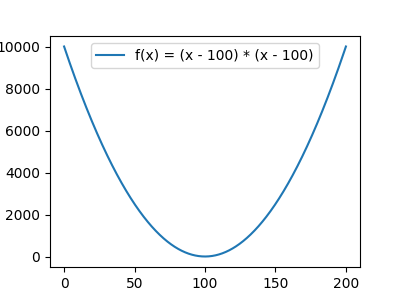
\includegraphics[width=0.65\textwidth]{images/parabola_positive.png}
		\caption{positive Funktion.}
		\label{pos_par}
	\end{minipage} \hfill
	\begin{minipage}{0.48\textwidth}
		\centering
		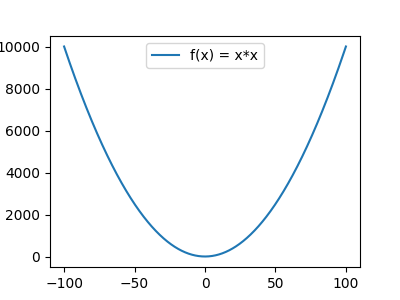
\includegraphics[width=0.65\textwidth]{images/parabola.png}
		\caption{quadratische Funktion.}
		\label{par}
	\end{minipage}
\end{figure}

Auf der ersten Grafik erkennt man, dass die X-Werten nur Positive sind. Ich werde jetzt einige Ergebnisse vorstellen und zeigen, ob die ANFIS-Modelle die Funktionen gleich lernen.

\subsection{Lernen der Parabelfunktion mit Mini-Batch Gradient Descent}

Zuerst betrachten wir zwei Modelle, die das Lernen über 10 Abläufe, bzw. 50 Iterationen, durchführen. Die Ergebnisse sind in den Abbildungen \ref{par_1000_50IT} und \ref{par_pos_1000_50IT} zu lesen.
\begin{figure}[htbp]
	\centering
	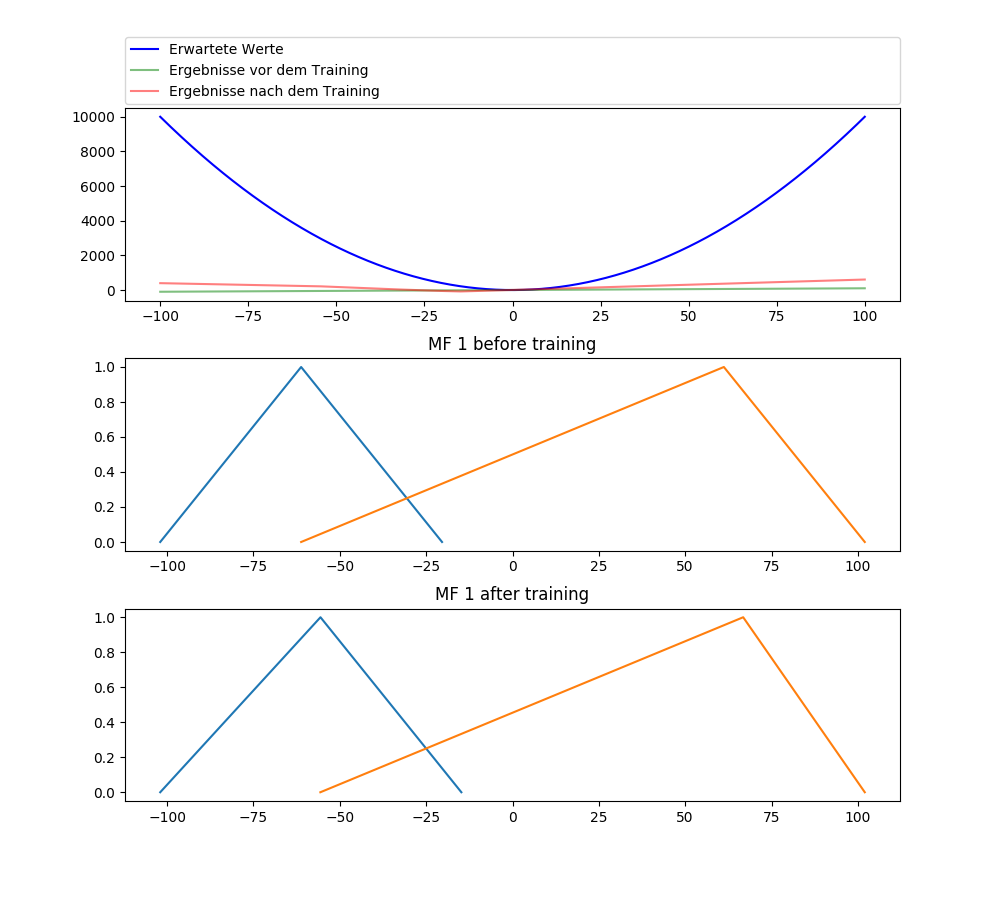
\includegraphics[width=0.65\textwidth]{images/parabola_1000/Mini-Batch/parabola_1000 1 Input 2 Sets 50 Epochs Mini-Batch Gradient Descent two equations mf.png}
	\caption{2 Fuzzy-Sets, 50 Iterationen, MF-Typ 0}
	\label{par_1000_50IT}
\end{figure}
\begin{figure}[htbp]
	\centering
	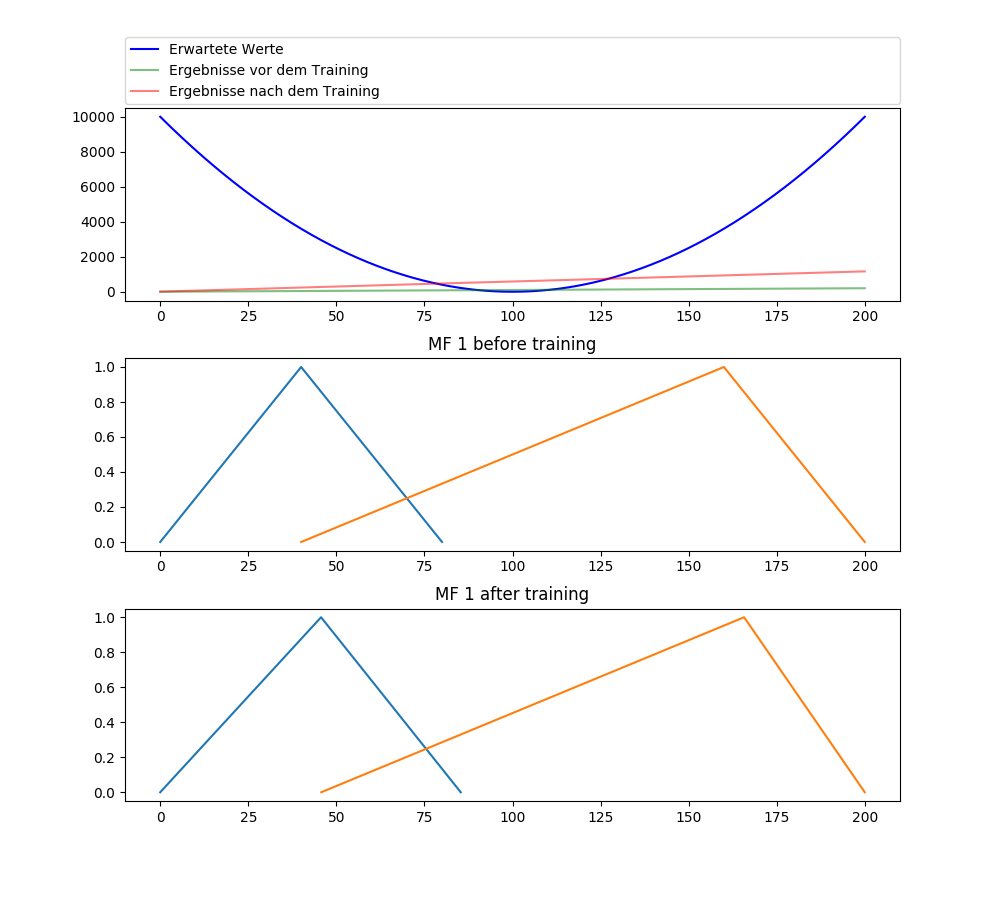
\includegraphics[width=0.65\textwidth]{images/parabola_positive/Mini-Batch/parabola_positive 1 Input 2 Sets 50 Epochs Mini-Batch Gradient Descent two equations mf.png}
	\caption{2 Fuzzy-Sets, 50 Iterationen, MF-Typ 0 mit nur Positiven X-Werte}
	\label{par_pos_1000_50IT}
\end{figure}

In diesem Fall ist die Anzahl der Durchläufe viel zu klein, um wesentliche Ergebnisse geliefert zu werden. Man erkennt, dass in der Grafik \ref{par_1000_50IT} die zwei Enden der Kurve nach oben geschoben sind, während die Mitte auf dem 0-Punkt liegt. In der Grafik \ref{par_pos_1000_50IT} erkennt man keine Kurve wirklich, sondern eine Gerade, welche die selbe wie der Ursprungsgerade ist, aber versetzt. Es werden die nummerische Unterschiede der beiden Modellen in der Tabelle \ref{par_tab1_50MB} betrachtet:

\begin{center}
	\begin{minipage}{\textwidth}
	\begin{tabular}{ | p{3.1cm} | l | l | p{3cm} | p{3cm} |}
		\hline
		Type & Time & Error & Gradient Type & MF Type \\ \hline
		parabola\_1000 & 0.27263559800000037 & 17675046.0 & Mini-Batch Gradient Descent & two equations mf
		 \\ \hline
		parabola\_positive & 0.26520074800000026 & 16615864.0 & Mini-Batch Gradient Descent & two equations mf
		 \\ \hline
	\end{tabular}
\captionof{table}{Testergebnisse für die Modelle}\label{par_tab1_50MB}
\end{minipage}
\end{center} 

Aus der Tebelle \ref{par_tab1_50MB} erkennt man, dass das ``positive'' Modell sowohl schneller als auch ``richtiger'' ist. Die Bilder würden deuten, dass das ``normale'' Model besser ist, aber die nummerischen Daten sagen, dass das andere Modelle das bessere wäre. Das nächste Beipsiel beantwortet die Frage, welche Aufgabe besser gelernt werden kann.

Als nächstes werden wir die zwei Modellen 1000 Mal laufen lassen, das würde heißen das es insgesammt 5000 Iterationen durchgeführt werden. Die weiteren Konfigurationen verbleiben gleich. Zuerst werden die Abbildung \ref{par_5000It} und \ref{par_pos_5000It} aus den beiden Tests gegeben:

\begin{figure}[htbp]
	\begin{minipage}{\textwidth}
	
	\centering
	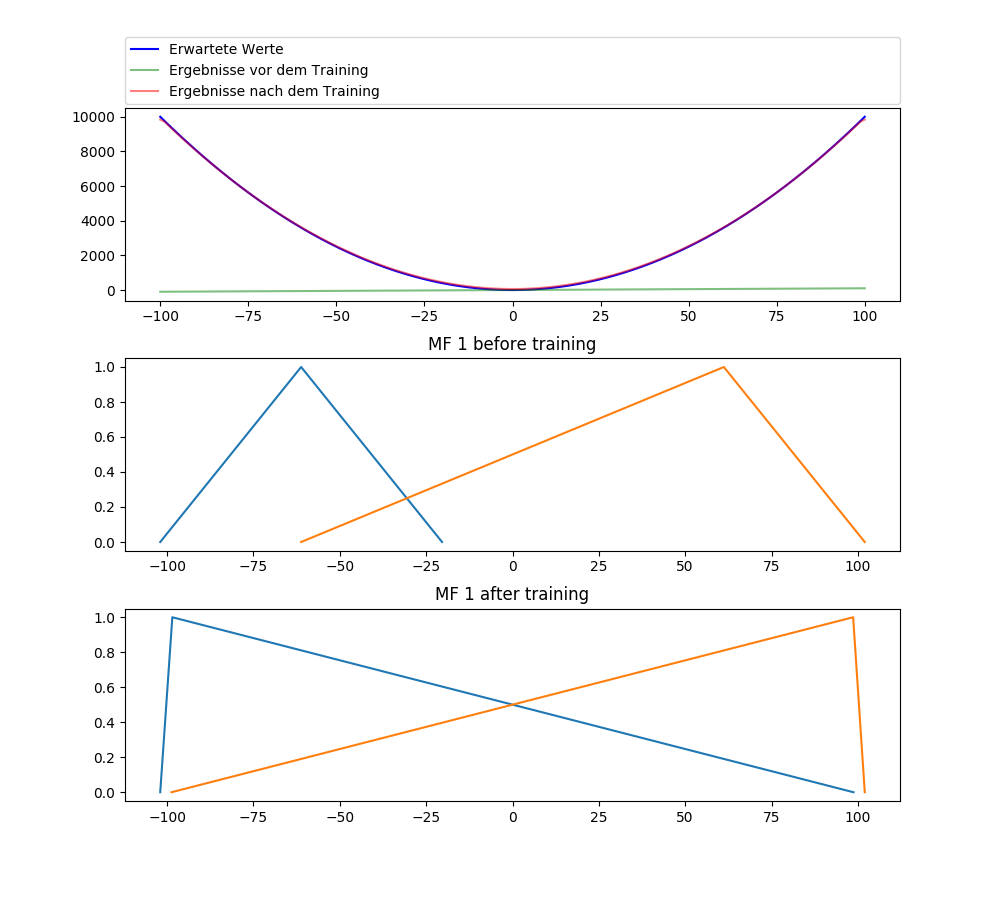
\includegraphics[width=0.65\textwidth]{images/parabola_1000/Mini-Batch/parabola_1000 1 Input 2 Sets 5000 Epochs Mini-Batch Gradient Descent two equations mf.png}
	\caption{2 Fuzzy-Sets, 5000 Iterationen, MF-Typ 0}
	\label{par_5000It}
\end{minipage}
\end{figure}
\begin{figure}[htbp]
	\begin{minipage}{\textwidth}
	
	\centering
	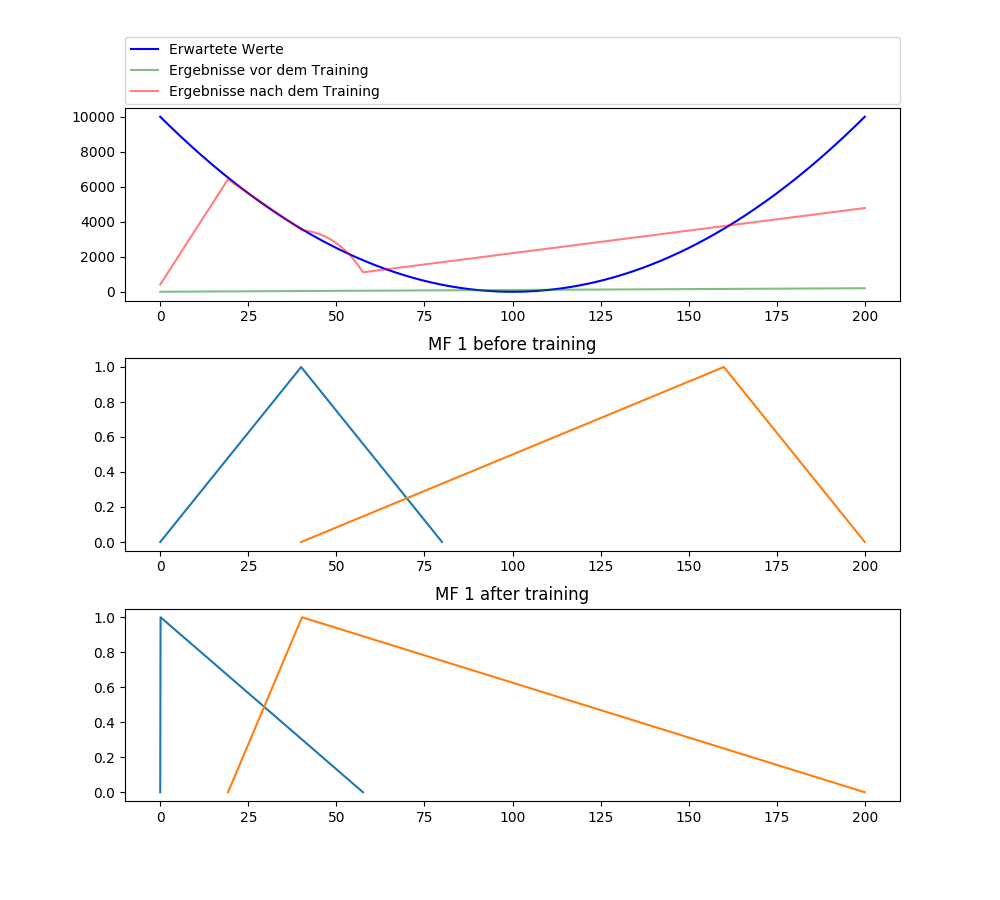
\includegraphics[width=0.65\textwidth]{images/parabola_positive/Mini-Batch/parabola_positive 1 Input 2 Sets 5000 Epochs Mini-Batch Gradient Descent two equations mf.png}
	\caption{2 Fuzzy-Sets, 5000 Iterationen, MF-Typ 0 mit nur Positiven X-Werte}
	\label{par_pos_5000It}
\end{minipage}
\end{figure}

Aus den Abbildungen ist zu lesen, dass das Modell (siehe \ref{par_5000It}) mit positiven und negativen Trainingsdaten schneller den Optimalzustand erreicht als das positve Modell. Außerdem nach 5000 Iterationen ist das Netz sehr gut trainiert. Es ist zu erwarten, dass die nummerische Daten auch für das erste Beispiel sprechen. Die Tabelle \ref{par_tab1_5000MB} beinhaltet die nummerischen Daten.

\begin{center}
	\begin{minipage}{\textwidth}
		
	
	\begin{tabular}{ | p{3.1cm} | l | l | p{3cm} | p{3cm} |}
		\hline
		Type & Time & Error & Gradient Type & MF Type \\ \hline
		parabola\_1000 & 12.538009995&1682.427&Mini-Batch Gradient Descent&two equations mf
		\\ \hline
		parabola\_positive & 12.474743275000002&5956089.5&Mini-Batch Gradient Descent&two equations mf
		\\ \hline
	\end{tabular}
\captionof{table}{Testergebnisee von dem Training der Funktionen ``parabola'' und parabola\_``positive''}\label{par_tab1_5000MB}
\end{minipage}
\end{center}

Wie auch schon aus den Grafiken ersichtlich geworden ist, eignet sich das Modell im positiven und negativen X-Bereich besser zum lernen. Auch die nummerischen Daten sprechen dafür, dass dies der Fall ist. Es besteht ein riesiger Unterschied in den Fehlerraten der beiden Testfälle.

\section{Fazit}

Die beschriebenen Testfälle wurden explizit ausgewählt, mit dem Ziel bestimmte Eigenschaften nachzuweisen. Der durchgeführten Tests zofolge kann beschlossen werden, dass nur Modelle mit dem MF-Typ 0 (siehe \ref{mf_typ0}) unterstützt sind.

Es ist sehr wichtig zu erwähnen, dass die Vergrößerung um eine Zusätzliche Menge etwa zwischen 1,2 und 1,3 Mal mehr Laufzeit erfordert. Während einer Verdopplung in Iterationen etwa die doppelte Laufzeit erfordert, was auch zu erwarten ist. Die Abbildung \ref{mini_batch_parabel_grafik} zeigt diese Beziehung.

\begin{figure}[htbp]
	\centering
	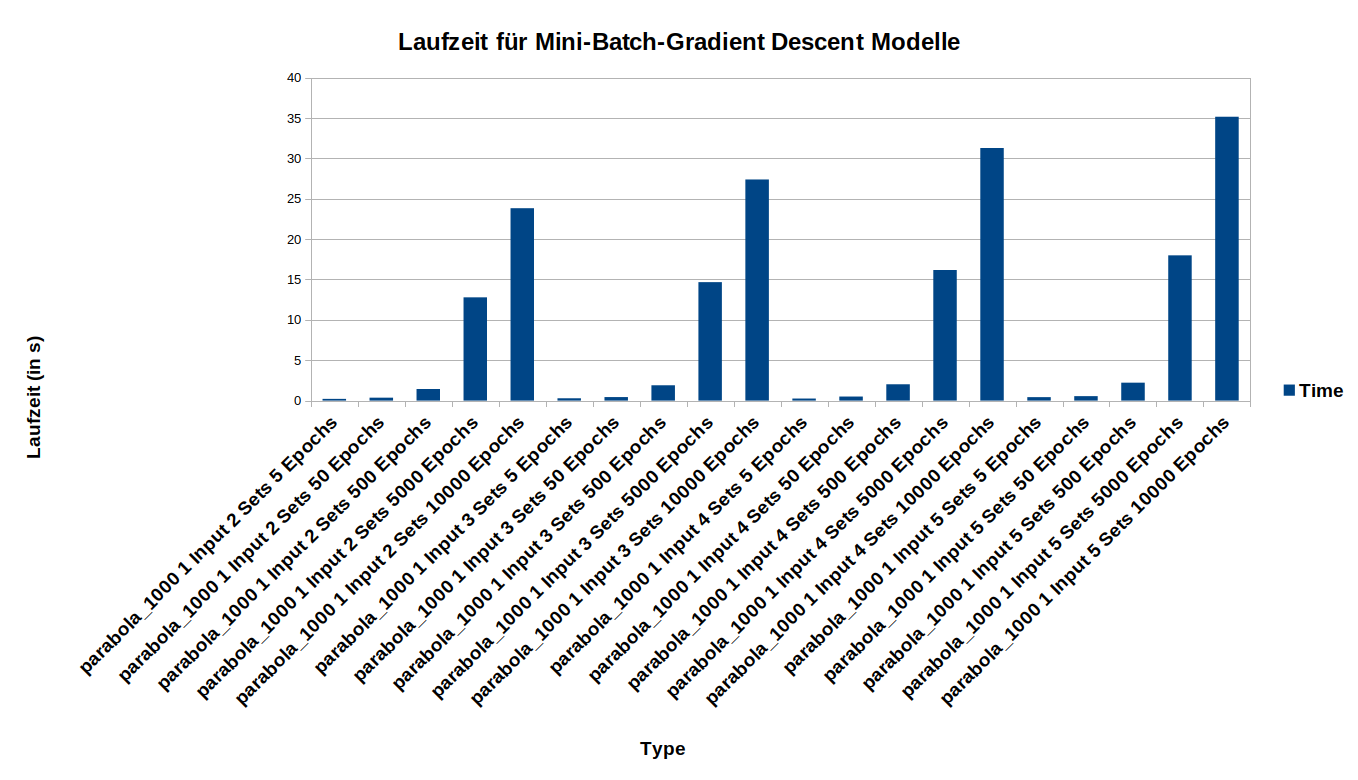
\includegraphics[width=1\textwidth]{images/charts/Mini-BatchGradientTimeParabola_bold.png}
	\caption{Laufzeit für Modelle beim Erlernen der Parabel Funktion}
	\label{mini_batch_parabel_grafik}
\end{figure}

Weiterhin ist es sehr wichtig zu betonen, dass das Lernen mit Mini-Batch und Batch Gradient Descent die bessere Option im vergleich zum Stochastic-Verfahren sind. Einer der Gründe dafür ist, weil es eine bessere Fehlerrate in kleineren Laufzeiten erzielt wird. Diese Behauptung wird durch die nächsten zwei Abbildungen \ref{best_sinus} und \ref{best_parabola}.

\begin{figure}[htbp]
	\centering
	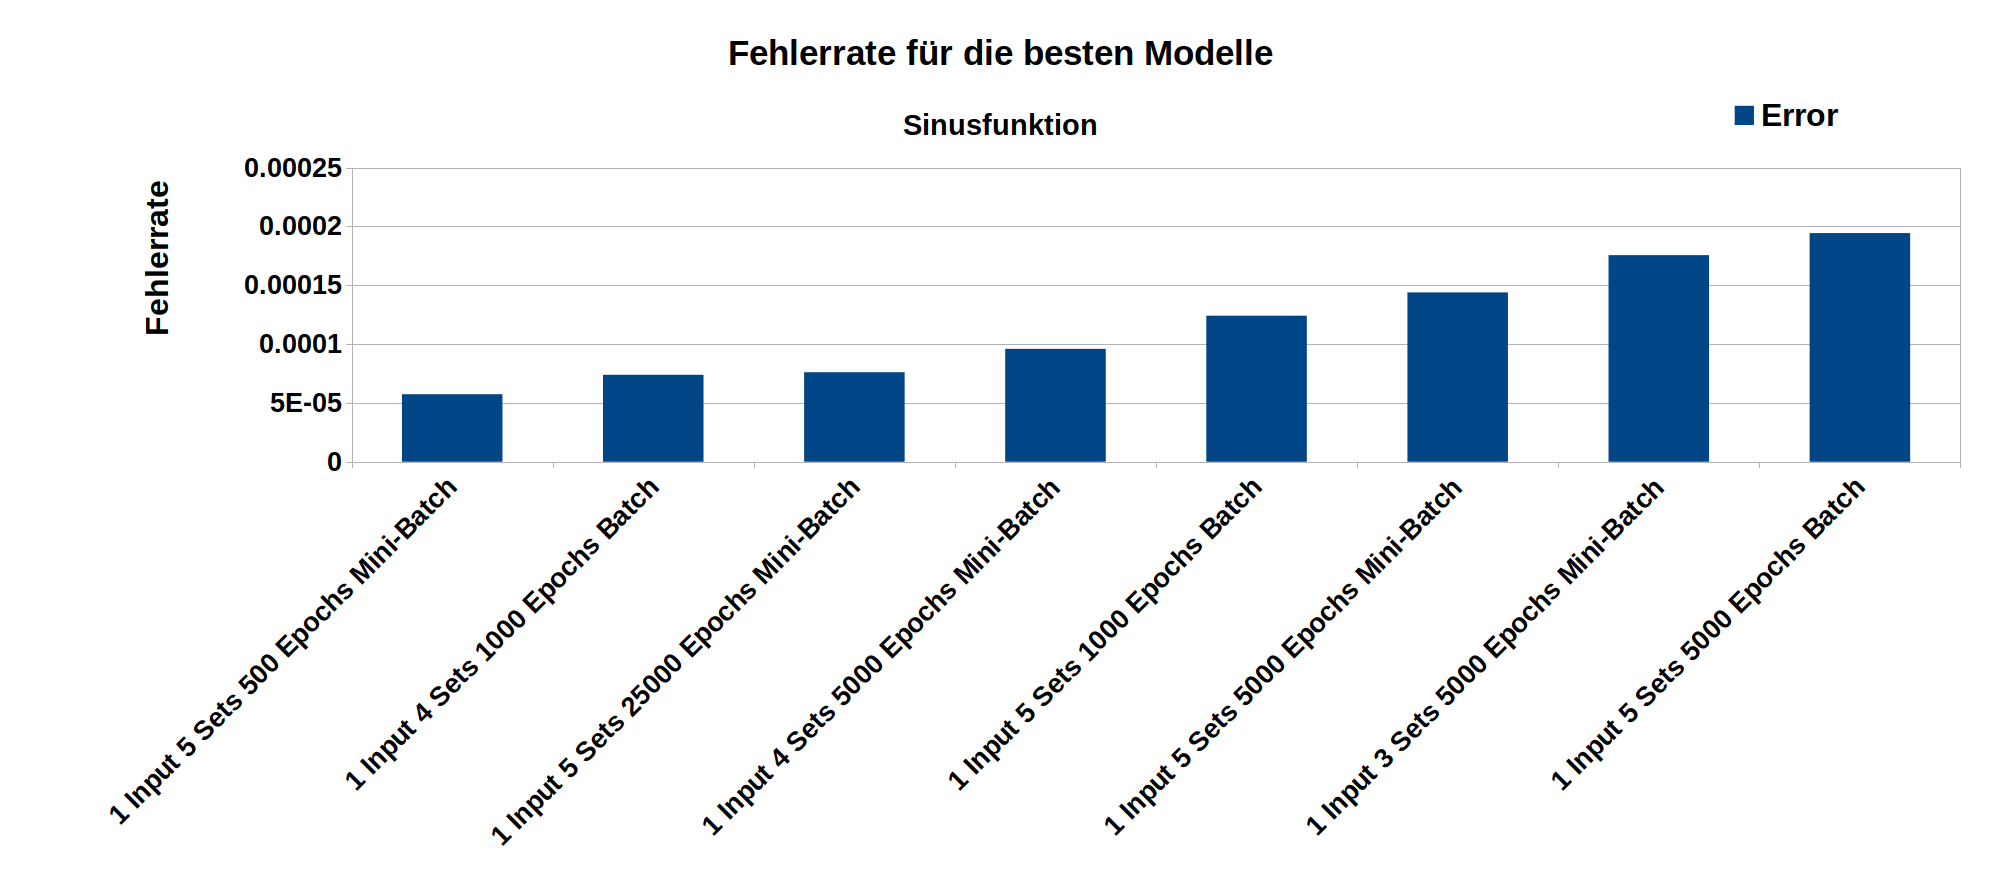
\includegraphics[width=1\textwidth]{images/charts/SinusFunktionbesteModelle_bold.png}
	\caption{Die besten Modelle beim Lernen der Sinusfunktion}
	\label{best_sinus}
\end{figure}

\begin{figure}[htbp]
	\centering
	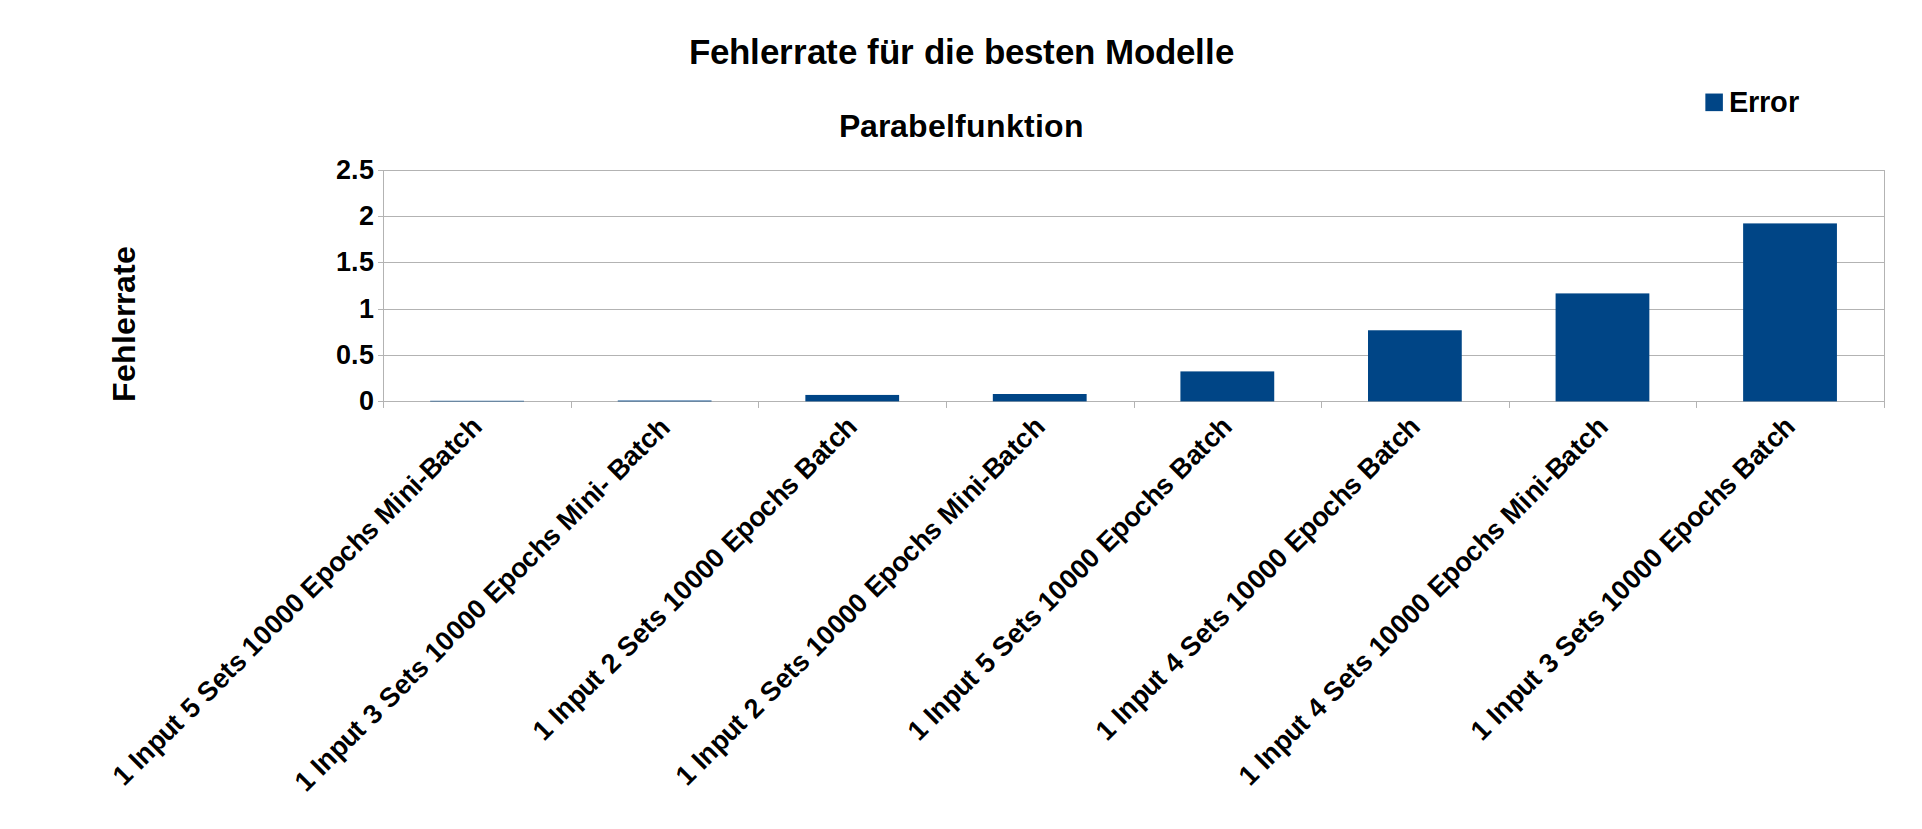
\includegraphics[width=1\textwidth]{images/charts/ParabelFunktionbesteModelle_bold.png}
	\caption{Laufzeit für Modelle beim Erlernen der Parabel Funktion}
	\label{best_parabola}
\end{figure}

Das weitere, was aus den Abbildung \ref{best_sinus} und \ref{best_parabola} zu entnehmen ist, ist, dass der Stochastische Verfahren in keinen der beiden Abbildungen figuriert. Das schließt dieses Verfahren zum Lernen der beiden Funktionen aus.

Aus den beiden Abbildungen \ref{best_sinus} und \ref{best_parabola} kommt man zu der Schlussfolgerung, dass das Mini-Batch-Verfahren bei dem Lernen von beiden Funktionen besser ist. 
%Die Tabelle \ref{best_table} verschafft weitere Informationen dafür, wie die besten Parabel-Modelle in Bezug auf die Laufzeit zueinander im Vergleich stehen.
%
%\begin{center}
%	\begin{minipage}{\textwidth}
%		
%		
%		\begin{tabular}{ | p{3.1cm} | l | l | p{3cm} | p{3cm} |}
%			\hline
%			Type & Time & Error & Gradient Type & MF Type \\ \hline
%			parabola 1 Input 5 Sets 10000 Epochs& 35.160331928& 0.0058110915& Mini-Batch& two equations mf \\ \hline
%			parabola 1 Input 3 Sets 10000 Epochs& 27.390405662& 0.008686484& Mini-Batch& two equations mf \\ \hline
%			parabola 1 Input 2 Sets 10000 Epochs& 22.068964008& 0.06951212& Batch& two equations mf \\ \hline
%			parabola 1 Input 2 Sets 10000 Epochs& 23.82696547& 0.07919865& Mini-Batch& two equations mf \\ \hline
%			parabola 1 Input 5 Sets 10000 Epochs& 36.840694511&  0.32366803& Batch& two equations mf \\ \hline
%			parabola 1 Input 4 Sets 10000 Epochs& 32.4242043& 0.7675758& Batch& two equations mf \\ \hline
%			parabola 1 Input 4 Sets 10000 Epochs& 31.288911103& 1.166094& Mini-Batch& two equations mf \\ \hline
%			parabola 1 Input 3 Sets 10000 Epochs& 27.11144164 & 1.9211318 & Batch&two equations mf \\ \hline
%		\end{tabular}
%		\captionof{table}{Beste Modelle beim Lernen der Parabelfunktion}\label{best_table}
%	\end{minipage}
%\end{center}
%
%Laut der Tabelle \ref{best_parabola} lassen sich keine Schlüsse dafür ziehen, welches Gradienten-Verfahren schneller ist, da in manchen Fällen ist es das Mini-Batch- (Vgl. 1. und 5. Zeile in der Tabelle) und anderen das Batch-Verfahren (Vgl. 2. und 8. Zeile in der Tabelle).  

%Das implementierte von mir Programm unterstützt auch Fuzzy-Systeme mit mehr elementiger Eingabe. Diese Funktionalität wurde jedoch nicht ausführlich getestet und somit auch nicht dokumentiert, weil mein Schwerpunkt in der Untersuchung des Modells lag. Außerdem wurde meine Konzentration auf das Erlernen Neuronaler Netze und genauer Tensorflow gerichtet. Am Ende dieser Arbeitung kann ich für mich sagen, dass ich die genannten Aspekte erfüllt habe und die gesammelten Erfahrungen für mich sehr in der Zukunft sehr wichtig sein werden.



%\chapter{LaTeX-Bausteine}\label{Stile}

Der Text wird in bis zu drei Ebenen gegliedert:

\begin{enumerate}
  \item Kapitel ( \verb \chapter{Kapitel} ), \index{Kapitel}
  \item Unterkapitel  ( \verb \section{Abschnitt} ) und
  \item Unterunterkapitel  ( \verb \subsection{Unterabschnitte} ).
\end{enumerate}

\section{Abschnitt}\index{Abschnitt}
Text der Gliederungsebene 2.


\subsection{Unterabschnitt} \index{Unterabschnitt}
Text der Gliederungsebene 3.
Text Text Text Text Text Text Text Text Text Text Text Text Text Text Text
Beispiel f�r Quelltext\index{Quelltext} \\[2 ex]
\noindent
\begin{minipage}{1.0\textwidth} \small
\begin{lstlisting}
	Prozess 1:
	
	Acquire();
		a := 1;
	Release();
	...
	Acquire();
	if(b == 0)
	{					
		c := 3;
		d := a;
	}				
	Release();
\end{lstlisting}
\end{minipage}

\vspace{2cm}
\noindent
\begin{minipage}{1.0\textwidth} \small
\begin{lstlisting}
	Prozess 2:
	
	Acquire();
		b := 1;
	Release();
	...
	Acquire();
	if(a == 0)
	{					
		c := 5;
		d := b;
	}				
	Release();
\end{lstlisting}
\end{minipage}
\vskip 1em

Gr��ere Code-Fragmente sollten im Anhang eingef�gt werden.

\section{Abbildungen und Tabellen}

Abbildung\index{Abbildung} und Tabellen\index{Tabelle} werden zentriert eingef�gt. Grunds�tzlich sollen sie
erst dann erscheinen, nach dem sie im Text angesprochen wurden (siehe Abb. \ref{a1}). Abbildungen und Tabellen (siehe Tabelle \ref{t1}) k�nnen
im (flie�enden) Text (\verb here ), am Seitenanfang (\verb top ), am Seitenende
(\verb bottom ) oder auch gesammelt auf einer nachfolgenden Seite (\verb page )
oder auch ganz am Ende der Ausarbeitung erscheinen. Letzteres sollte man nur
dann w�hlen, wenn die Bilder g�nstig zusammen zu betrachten sind und die
Ausarbeitung nicht zu lang ist ($< 20$ Seiten).

\begin{figure} %[hbtp]
	\centering
		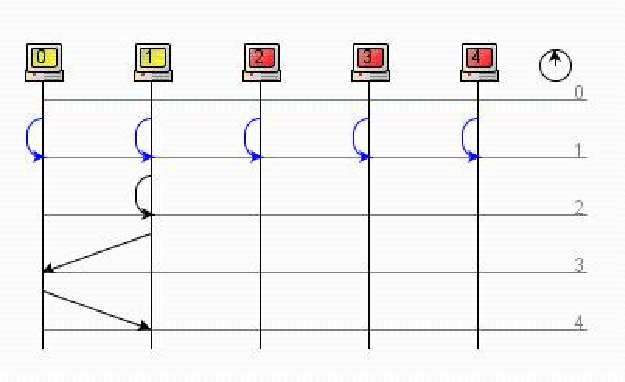
\includegraphics{images/p1ReadSeq.pdf}
	\caption{Bezeichnung der Abbildung}
	\label{a1}
\end{figure}

\begin{table} %[hbtp]
	\centering
		\begin{tabular}{l | l l l l}
		\textbf{Prozesse} & \textbf{Zeit} $\rightarrow$ \\
		\hline
			$P_{1}$ & $W(x)1$ \\
			$P_{2}$ & & $W(x)2$ \\
			$P_{3}$ & & $R(x)2$ & & $R(x)1$\\
			$P_{4}$ & & & $R(x)2$ & $R(x)1$\\
		\end{tabular}
	\caption{Bezeichnung der Tabelle}
	\label{t1}
\end{table}


\section{Mathematische Formel}\index{Formel}
Mathematische Formeln bzw. Formulierungen k�nnen sowohl im
laufenden Text (z.B. $y=x^2$) oder abgesetzt und zentriert im Text
erscheinen. Gleichungen sollten f�r Referenzierungen nummeriert
werden (siehe Formel \ref{gl-1}).
\begin{equation}
\label{gl-1}
e_{i}=\sum _{i=1}^{n}w_{i}x_{i}
\end{equation}

Entscheidungsformel:

\begin{equation}
\psi(t)=\left\{\begin{array}{ccc}
1 &  \qquad 0 <= t < \frac{1}{2} \\
-1 &  \qquad \frac{1}{2} <= t <1 \\
0 & \qquad sonst
\end{array} \right.
\end{equation}


Matrix:\index{Matrix}
\begin{equation}
A = \left(
\begin{array}{llll}
a_{11} & a_{12} & \ldots & a_{1n} \\
a_{21} & a_{22} & \ldots & a_{2n} \\
\vdots & \vdots & \ddots & \vdots \\
a_{n1} & a_{n2} & \ldots & a_{nn} \\
\end{array}
\right)
\end{equation}

Vektor:\index{Vektor} 

\begin{equation}
\overline{a} = \left(
\begin{array}{c}
a_{1}\\
a_{2}\\
\vdots\\
a_{n}\\
\end{array}
\right)
\end{equation}

\section{S�tze, Lemmas und Definitionen}\index{Satz}\index{Lemma}\index{Definition}

S�tze, Lemmas, Definitionen, Beweise,\index{Beweis} Beispiele\index{Beispiel} k�nnen in speziell daf�r vorgesehenen Umgebungen erstellt werden.

\begin{definition}(Optimierungsproblem)

Ein \emph{Optimierungsproblem} $\mathcal{P}$ ist festgelegt durch ein Tupel
$(I_\mathcal{P}, sol_\mathcal{P}, m_\mathcal{P}, goal)$ wobei gilt

\begin{enumerate}
\item $I_\mathcal{P}$ ist die Menge der Instanzen,
\item $sol_\mathcal{P} : I_\mathcal{P} \longmapsto \mathbb{P}(S_\mathcal{P})$ ist eine Funktion, die jeder Instanz $x \in I_\mathcal{P}$ eine Menge zul�ssiger L�sungen zuweist,
\item $m_\mathcal{P} : I_\mathcal{P} \times S_\mathcal{P} \longmapsto \mathbb{N}$ ist eine Funktion, die jedem Paar $(x,y(x))$ mit $x \in I_\mathcal{P}$ und $y(x) \in sol_\mathcal{P}(x)$ eine
Zahl $m_\mathcal{P}(x,y(x)) \in \mathbb{N}$ zuordnet (= Ma� f�r die L�sung $y(x)$ der Instanz $x$), und
\item $goal \in \{min,max\}$.
\end{enumerate}

\end{definition}

\begin{example} MINIMUM TRAVELING SALESMAN (MIN-TSP)
\begin{itemize}
\item $I_{MIN-TSP} =_{def}$ s.o., ebenso $S_{MIN-TSP}$
\item $sol_{MIN-TSP}(m,D) =_{def} S_{MIN-TSP} \cap \mathbb{N}^m$ 
\item $m_{MIN-TSP}((m,D),(c_1, \ldots , c_m)) =_{def} \sum_{i=1}^{m-1} D(c_i, c_{i+1}) + D(c_m,c_1)$ 
\item $goal_{MIN-TSP} =_{def} min$
\end{itemize}
\begin{flushright}
$\qed$
\end{flushright}
\end{example}

\begin{theorem} Sei $\mathcal{P}$ ein \textbf{NP}-hartes Optimierungsproblem.
Wenn $\mathcal{P} \in$ \textbf{PO}, dann ist \textbf{P} = \textbf{NP}.
\end{theorem}

\begin{proof} Um zu zeigen, dass \textbf{P} = \textbf{NP} gilt, gen�gt es
wegen Satz A.30 zu zeigen, dass ein einziges \textbf{NP}-vollst�ndiges
Problem in \textbf{P} liegt. Sei also $\mathcal{P}'$ ein beliebiges \textbf{NP}-vollst�ndiges Problem.

Weil $\mathcal{P}$ nach Voraussetzung \textbf{NP}-hart ist, gilt insbesondere
$\mathcal{P}' \leq_T \mathcal{P}_C$. Sei $R$ der zugeh�rige
Polynomialzeit-Algorithmus dieser Turing-Reduktion.
Weiter ist $\mathcal{P} \in$ \textbf{PO} vorausgesetzt, etwa verm�ge eines
Polynomialzeit-Algorithmus $A$. Aus den beiden
Polynomialzeit-Algorithmen $R$ und $A$ erh�lt man nun
leicht einen effizienten Algorithmus f�r $\mathcal{P}'$: Ersetzt man
in $R$ das Orakel durch $A$, ergibt dies insgesamt eine polynomielle
Laufzeit. 
%\begin{flushright}
$\qed$
% \end{flushright}
\end{proof}

\begin{lemma} Aus \textbf{PO} $=$ \textbf{NPO} folgt \textbf{P} $=$ \textbf{NP}.
\end{lemma}

\begin{proof} Es gen�gt zu zeigen, dass unter der angegeben
Voraussetzung KNAPSACK $\in$ \textbf{P} ist.

Nach Voraussetung ist MAXIMUM KNAPSACK $\in$ \textbf{PO},
d.h. die Berechnung von $m^*(x)$ f�r jede Instanz $x$ ist
in Polynomialzeit m�glich. Um KNAPSACK bei Eingabe
$(x,k)$ zu entscheiden, m�ssen wir nur noch $m^*(x) \geq k$
pr�fen. Ist das der Fall, geben wir $1$, sonst $0$ aus. Dies
bleibt insgesamt ein Polynomialzeit-Algorithmus. 
\begin{flushright}
$\qed$
\end{flushright}
\end{proof}

\section{Fu�noten}

In einer Fu�note k�nnen erg�nzende Informationen\footnote{Informationen die f�r die Arbeit zweitrangig sind, jedoch f�r den Leser interessant sein k�nnten.} angegeben werden. Au�erdem kann eine Fu�note auch Links enthalten. Wird in der Arbeit eine Software (zum Beispiel Java-API\footnote{\url{http://java.sun.com/}}) eingesetzt, so kann die Quelle, die diese Software zur Verf�gung stellt in der Fu�note angegeben werden.

\section{Literaturverweise}\index{Literatur}
Alle benutzte Literatur wird im Literaturverzeichnis angegeben\footnote{Dazu wird ein sogennanter bib-File, literatur.bib verwendet.}. Alle angegebene Literatur sollte mindestens einmal im Text referenziert werden\cite{Coulouris:02}.
%\chapter{Beispiel-Kapitel}

In diesem Kapitel wird beschrieben, warum es unterschiedliche Konsistenzmodelle\index{Konsistenzmodelle} gibt. Au�erdem werden die Unterschiede zwischen strengen Konsistenzmodellen\index{Linearisierbarkeit} (Linearisierbarkeit, sequentielle Konsistenz)\index{sequentiell!Konsistenz} und schwachen Konsistenzmodellen\index{Konsistenz!schwach} (schwache Konsistenz, Freigabekonsistenz)\index{Freigabekonsistenz} erl�utert. Es wird gekl�rt, was Strenge und Kosten (billig, teuer) in Zusammenhang mit Konsistenzmodellen bedeuten.

\section{Warum existieren unterschiedliche Konsistenzmodelle?}

Laut \cite{Malte:97} sind mit der\index{Replikation} Replikation von Daten immer zwei gegens�tzliche Ziele verbunden: die Erh�hung der\index{Verf�gbarkeit} Verf�gbarkeit und die Sicherung der\index{Konsistenz} Konsistenz der Daten. Die Form der Konsistenzsicherung bestimmt dabei, inwiefern das eine Kriterium erf�llt und das andere dementsprechend nicht erf�llt ist (Trade-off zwischen Verf�gbarkeit und der Konsistenz der Daten). Stark konsistente Daten sind stabil, das hei�t, falls mehrere Kopien der Daten existieren, d�rfen keine Abweichungen auftreten. Die Verf�gbarkeit der Daten ist hier jedoch stark eingeschr�nkt. Je schw�cher die Konsistenz wird, desto mehr Abweichungen k�nnen zwischen verschiedenen Kopien einer Datei auftreten, wobei die Konsistenz nur an bestimmten Synchronisationspunkten gew�hrleistet wird. Daf�r steigt aber die Verf�gbarkeit der Daten, weil sie sich leichter replizieren lassen.

Nach \cite{Mosberger:93} kann die Performanzsteigerung der schw�cheren Konsistenzmodelle wegen der Optimierung\index{Optimierung} (Pufferung, Code-Scheduling, Pipelines) 10-40 Prozent betragen. Wenn man bedenkt, dass mit der Nutzung der vorhandenen Synchronisierungsmechanismen schw�chere Konsistenzmodelle den Anforderungen der strengen Konsistenz gen�gen, stellt sich der h�here programmiertechnischer Aufwand bei der Implementierung der schw�cheren Konsistenzmodelle als ihr einziges Manko dar.

In \cite{Cheriton:85} ist beschrieben, wie man sich Formen von DSM vorstellen k�nnte, f�r die ein beachtliches Ma� an\index{Inkonsistenz} Inkonsistenz akzeptabel w�re. Beispielsweise k�nnte DSM verwendet werden, um die Auslastung von Computern in einem Netzwerk zu speichern, so dass Clients f�r die Ausf�hrung ihrer Applikationen die am wenigsten ausgelasteten Computer ausw�hlen k�nnen. Weil die Informationen dieser Art innerhalb k�rzester Zeit ungenau werden k�nnen (und durch die Verwendung der veralteten Daten keine gro�en Nachteile entstehen k�nnen), w�re es vergebliche M�he, sie st�ndig f�r alle Computer im System konsistent zu halten \cite{Coulouris:02}. Die meisten Applikationen stellen jedoch strengere Konsistenzanforderungen.

\section{Klassifizierung eines Konsistenzmodells}

Die zentrale Frage, die f�r die Klassifizierung\index{streng}\index{schwach} (streng oder schwach) eines Konsistenzmodells von Bedeutung ist \cite{Coulouris:02}: wenn ein Lesezugriff auf eine Speicherposition erfolgt, welche Werte von Schreibzugriffen auf diese Position sollen dann dem Lesevorgang bereitgestellt werden? Die Antwort f�r das schw�chste Konsistenzmodell lautet: von jedem Schreibvorgang, der vor dem Lesen erfolgt ist, oder in der "`nahen"' Zukunft, innerhalb des definierten Betrachtungsraums, erfolgten wird. Also irgendein Wert, der vor oder nach dem Lesen geschrieben wurde.

F�r das strengste Konsistenzmodell, Linearisierbarkeit (atomic consistency), stehen alle geschriebenen Werte allen Prozessoren sofort zur Verf�gung: eine Lese-Operation gibt den aktuellsten Wert zur�ck, der geschrieben wurde, bevor das Lesen stattfand. Diese Definition ist aber in zweierlei Hinsicht problematisch. Erstens treten weder Schreib- noch Lese-Operationen zu genau einem Zeitpunkt auf, deshalb ist die Bedeutung von "`aktuellsten"' nicht immer klar. Zweitens ist es nicht immer m�glich, genau festzustellen, ob ein Ereignis vor einem anderen stattgefunden hat, da es Begrenzungen daf�r gibt, wie genau Uhren in einem verteilten System synchronisiert werden k�nnen.

Nachfolgend werden einige Konsistenzmodelle absteigend nach ihrer Strenge vorgestellt. Zuvor m�ssen wir allerdings kl�ren, wie die Lese- und Schreibe-Operationen in dieser Ausarbeitung dargestellt werden.

Sei $x$ eine Speicherposition, dann k�nnen Instanzen dieser Operationen wie folgt ausgedr�ckt werden:
\begin{itemize}
	\item $R(x)a$ - eine Lese-Operation\index{Operation!Lese}, die den Wert $a$ von der Position $x$ liest.
	\item $W(x)b$ - eine Schreib-Operation\index{Operation!Schreib}, die den Wert $b$ an der Position $x$ speichert.
\end{itemize}

\section{Linearisierbarkeit\index{Linearisierbarkeit} (atomic consistency)}

Die Linearisierbarkeit im Zusammenhang mit DSM kann wie folgt definiert werden:
\begin{itemize}
	\item Die verzahnte Operationsabfolge findet so statt: wenn $R(x)a$ in der Folge vorkommt, dann ist die letzte Schreib-Operation, die vor ihr in der verzahnten Abfolge auftritt, $W(x)a$, oder es tritt keine Schreib-Operation vor ihr auf und $a$ ist der Anfangswert von $x$. Das bedeutet, dass eine Variable nur durch eine Schreib-Operation ge�ndert werden kann.
	\item Die Reihenfolge der Operationen in der Verzahnung ist konsistent zu den \underline{Echtzeiten}\index{Echtzeiten}, zu denen die Operationen bei der tats�chlichen Ausf�hrung aufgetreten sind.
\end{itemize}

Die Bedeutung dieser Definition kann an folgendem Beispiel (Tabelle \ref{tab:1}) nachvollzogen werden. Es sei angenommen, dass alle Werte mit $0$ vorinitialisiert sind.

\begin{table}
	\centering
		\begin{tabular}{l | l l l l}
			\textbf{Prozesse} & \textbf{Zeit} $\rightarrow$ & \\
			\hline
			$P_{1}$ & $W(x)1$ & & $W(y)2$ \\
			$P_{2}$ & & $R(x)1$ & & $R(y)2$ \\
		\end{tabular}
	\caption{Linearisierbarkeit ist erf�llt}
	\label{tab:1}
\end{table}

Hier sind beide Bedingungen erf�llt, da die Lese-Operationen den zuletzt geschriebenen Wert zur�ckliefern. Interessanter ist es, zu sehen, wann die Linearisierbarkeit verletzt ist.

\begin{table}
	\centering
		\begin{tabular}{l | l l l l}
		\textbf{Prozesse} & \textbf{Zeit} $\rightarrow$ \\
		\hline
		$P_{1}$ & $W(x)1$ & $W(x)2$ \\
		$P_{2}$ & & & \color{red} $R(x)0$ & \color{black} $R(x)2$ \\
		\end{tabular}
	\caption{Linearisierbarkeit ist verletzt, sequentielle Konsistenz ist erf�llt.}
	\label{tab:2}
\end{table}

In diesem Beispiel (Tabelle \ref{tab:2}) ist die Echtzeit-Anforderung verletzt, da der Prozess $P_{2}$ immer noch den alten Wert liest, obwohl er von Prozess $P_{1}$ bereits ge�ndert wurde. Diese Ausf�hrung w�re aber sequentiell konsistent (siehe kommender Abschnitt), da es eine Verzahnung der Operationen gibt, die diese Werte liefern k�nnte ($R(x)0$, $W(x)1$, $W(x)2$, $R(y)2$). W�rde man beide Lese-Operationen des 2. Prozesses vertauschen, wie in der Tabelle \ref{tab:3} dargestellt, so w�re keine sinnvolle Verzahnung mehr m�glich.

\begin{table}
	\centering
		\begin{tabular}{l | l l l l}
		\textbf{Prozesse} & \textbf{Zeit} $\rightarrow$ \\
		\hline
		$P_{1}$ & $W(x)1$ & $W(x)2$ \\
		$P_{2}$ & & & \color{red} $R(x)2$ &  \color{red} $R(x)0$ \\
			
		\end{tabular}
	\caption{Linearisierbarkeit und sequentielle Konsistenz sind verletzt.}
	\label{tab:3}
\end{table}

In diesem Beispiel sind beide Bedingungen verletzt. Selbst wenn die Echtzeit, zu der die Operationen stattgefunden haben, ignoriert wird, gibt es keine Verzahnung einzelner Operationen, die der Definition entsprechen w�rde.
%\chapter{Zusammenfassung und Ausblick}

In diesem Kapitel soll die Arbeit noch einmal kurz zusammengefasst werden. Insbesondere sollen die wesentlichen Ergebnisse Ihrer Arbeit herausgehoben werden. Erfahrungen, die z.B. Benutzer mit der Mensch-Maschine-Schnittstelle gemacht haben oder Ergebnisse von Leistungsmessungen sollen an dieser Stelle pr�sentiert werden. Sie k�nnen in diesem Kapitel auch die Ergebnisse oder das Arbeitsumfeld Ihrer Arbeit kritisch bewerten. W�nschenswerte Erweiterungen sollen als Hinweise auf weiterf�hrende Arbeiten erw�hnt werden.
% ...
%--------------------------------------------------------------------------
\backmatter                        		% Anhang
%-------------------------------------------------------------------------
\bibliographystyle{geralpha}			% Literaturverzeichnis
\bibliography{literatur}     			% BibTeX-File literatur.bib
%--------------------------------------------------------------------------
\printindex 							% Index (optional)
%--------------------------------------------------------------------------
\begin{appendix}						% Anh�nge sind i.d.R. optional
%   \chapter{Glossar}

\abbreviation{DisASTer}		{DisASTer (Distributed Algorithms Simulation Terrain), A platform for the Implementation of Distributed Algorithms}
\abbreviation{DSM}			{Distributed Shared Memory}
\abbreviation{AC}			{Linearisierbarkeit (atomic consistency)}
\abbreviation{SC}			{Sequentielle Konsistenz (sequential consistency)}
\abbreviation{WC}			{Schwache Konsistenz (weak consistency)}
\abbreviation{RC}			{Freigabekonsistenz (release consistency)}
			% Glossar   
%%\chapter{Anhang}
\chapter{Anhang}

\begin{figure}[htbp]
	\centering
	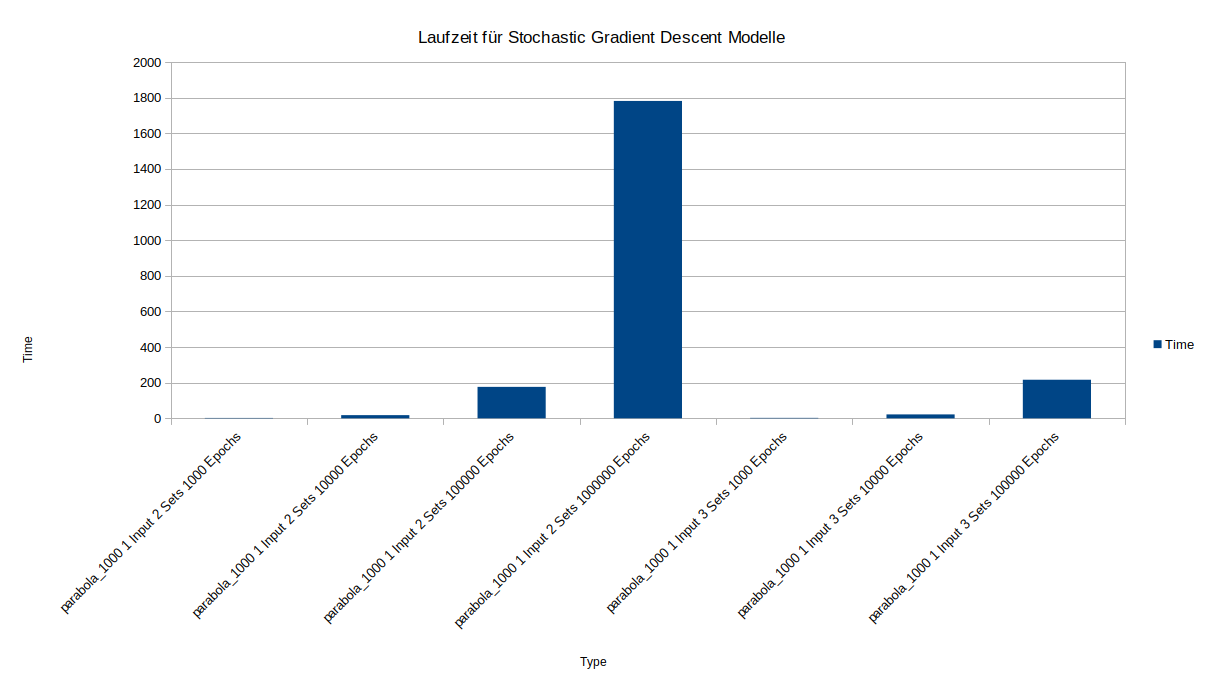
\includegraphics[angle=-90,totalheight=0.66\textheight]{images/charts/StochasticGradientTimeParabola.png}
	\caption{Laufzeit für Stochastic-Modelle beim Erlernen der Parabelfunktion}
\end{figure}

\begin{figure}[htbp]
	\centering
	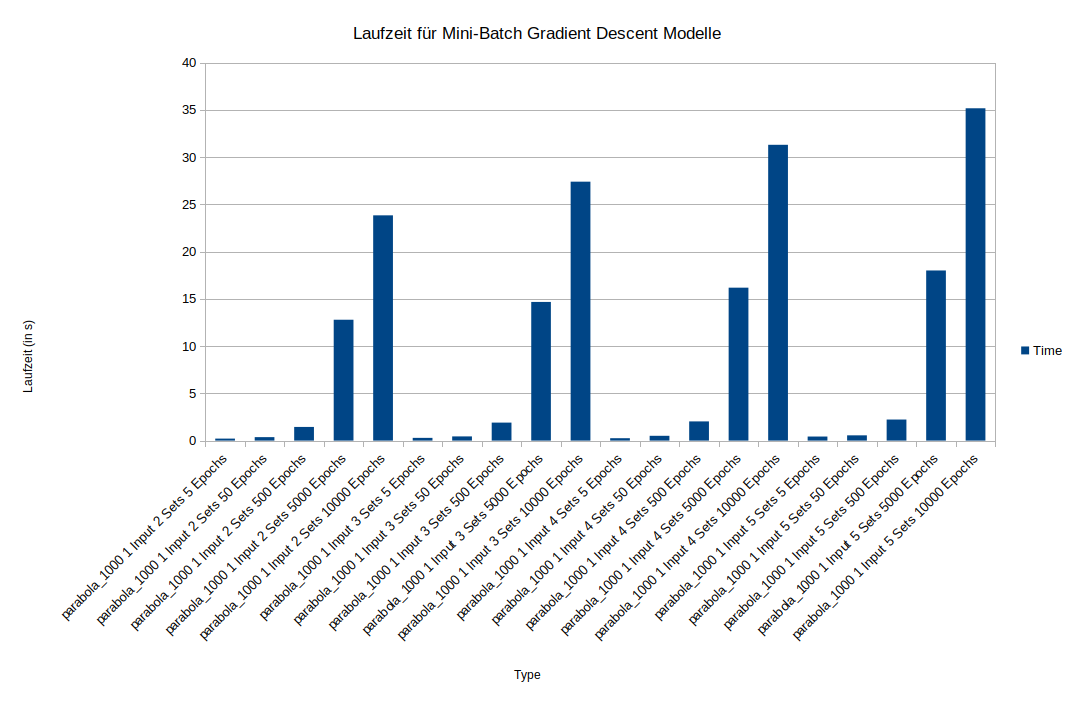
\includegraphics[angle=-90,totalheight=\textheight]{images/charts/Mini-BatchGradientTimeParabola.png}
	\caption{Laufzeit für Mini-Batch-Modelle beim Erlernen der Parabelfunktion}
\end{figure}

\begin{figure}[htbp]
	\centering
	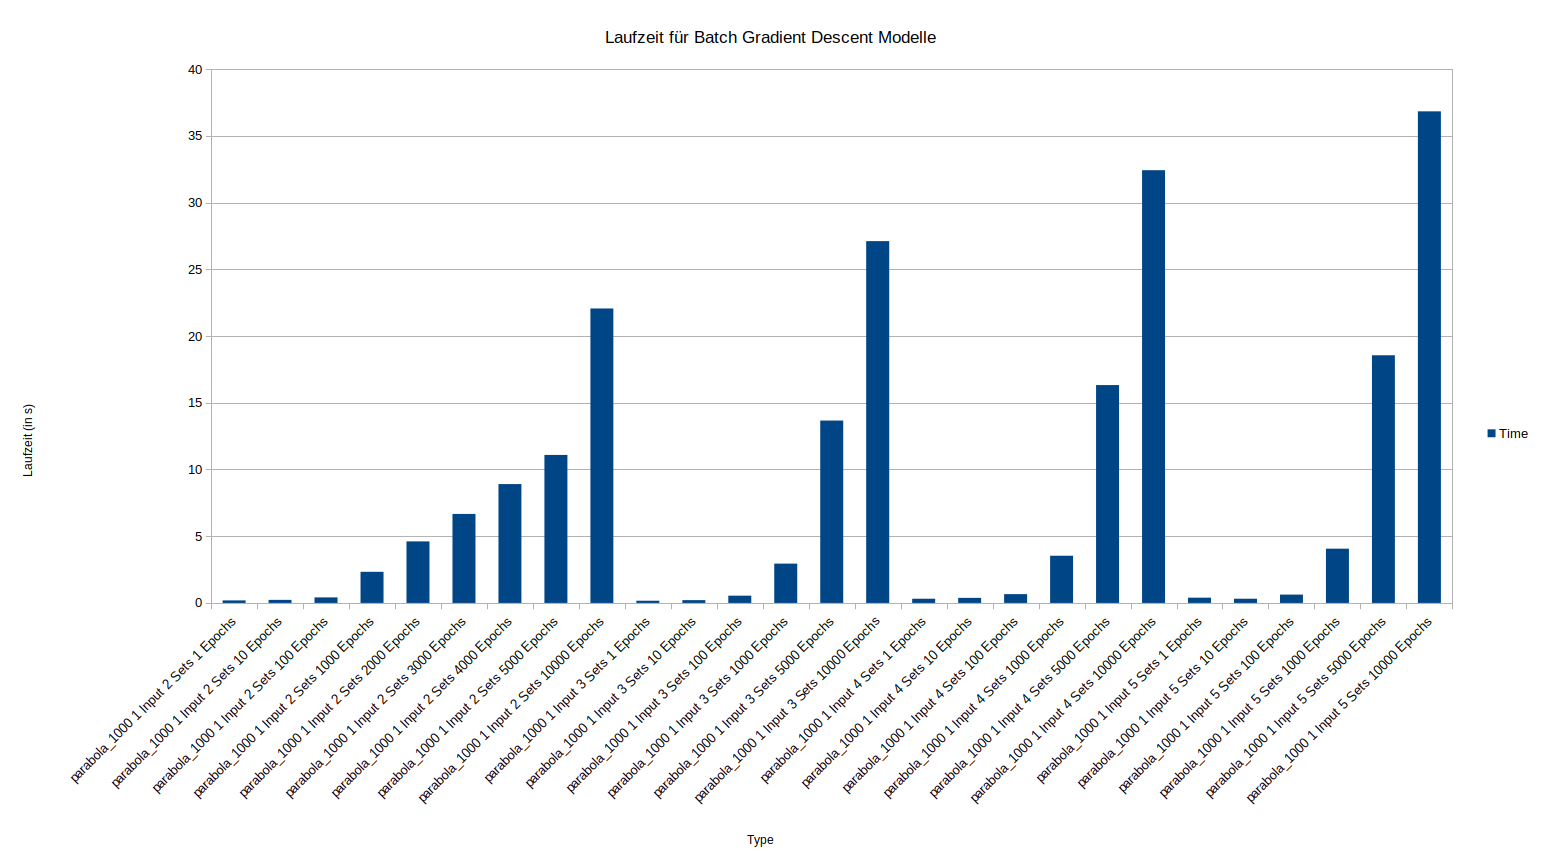
\includegraphics[angle=-90,totalheight=\textheight]{images/charts/BatchGradientTimeParabola.png}
	\caption{Laufzeit für Batch-Modelle beim Erlernen der Parabel Funktion}
\end{figure}

\begin{figure}[htbp]
	\centering
	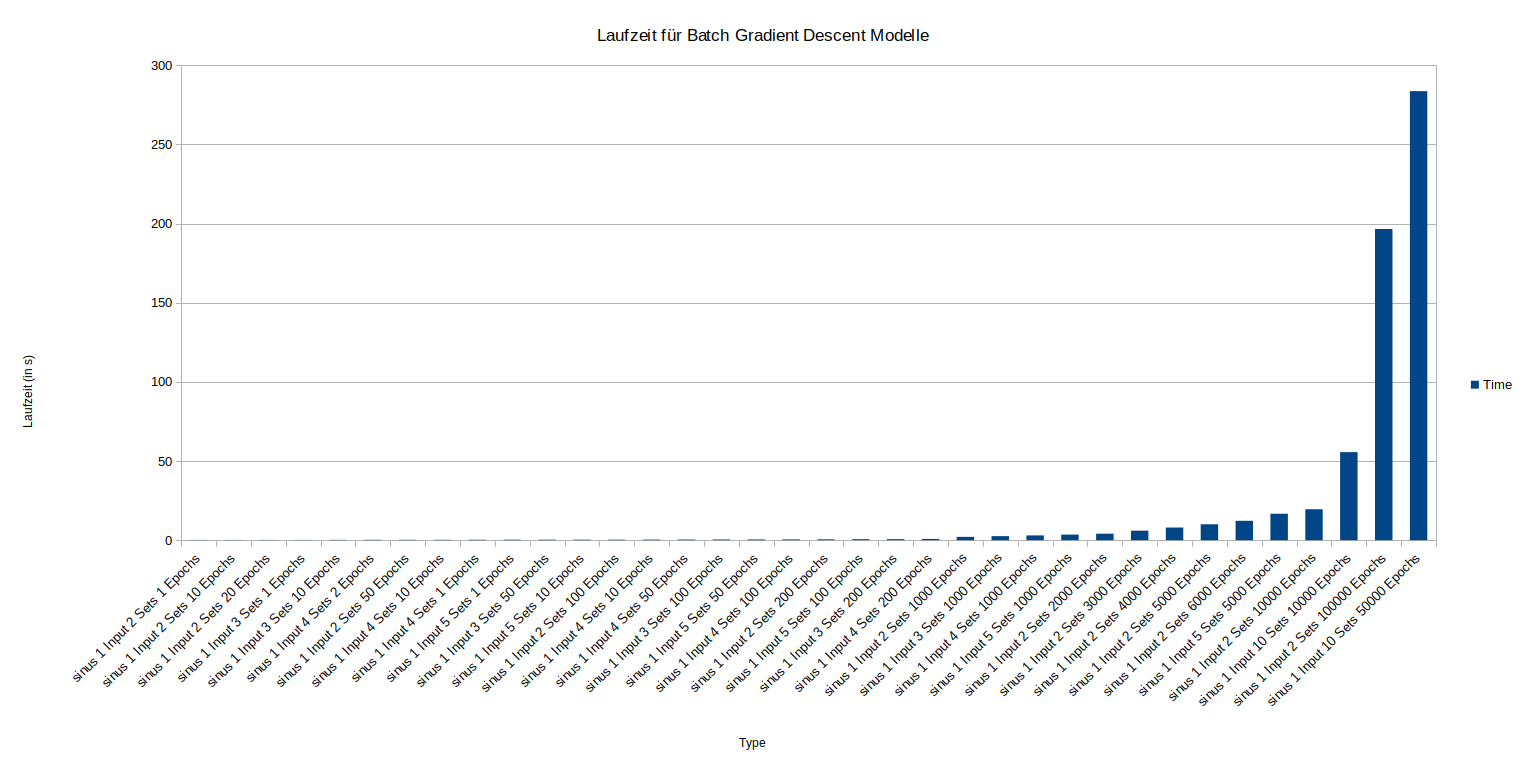
\includegraphics[angle=-90,totalheight=\textheight]{images/charts/BatchGradientTimeSinus.png}
	\caption{Laufzeit für Batch-Modelle beim Erlernen der Sinusfunktion}
\end{figure}

\begin{figure}[htbp]
	\centering
	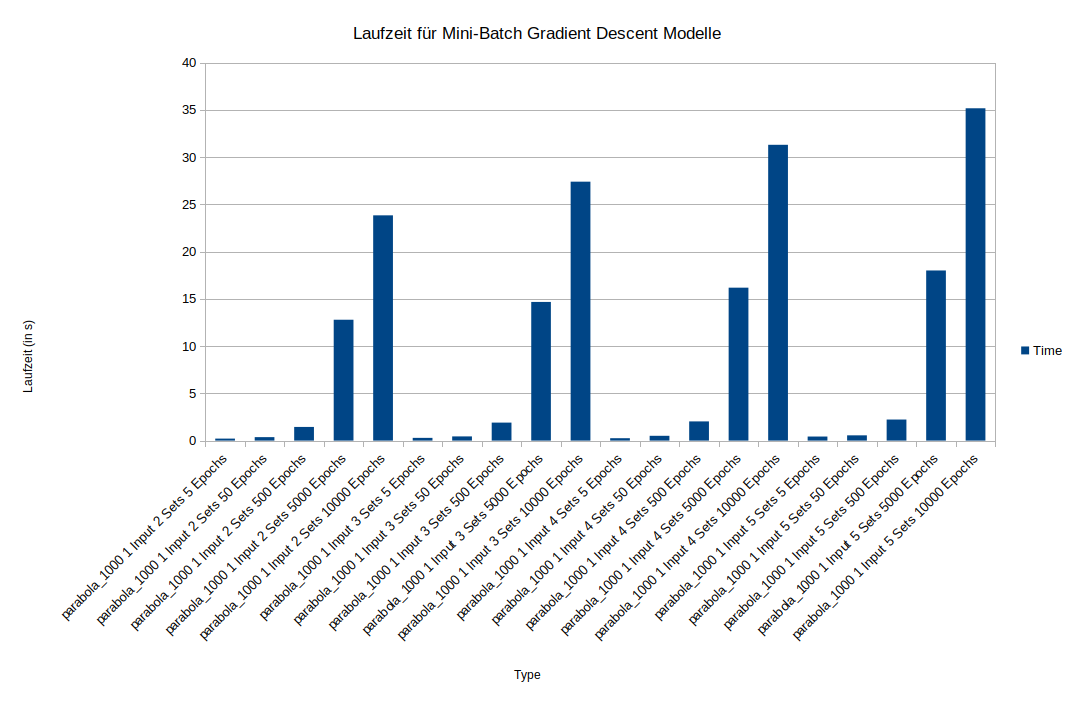
\includegraphics[angle=-90,totalheight=\textheight]{images/charts/Mini-BatchGradientTimeParabola.png}
	\caption{Laufzeit für Mini-Batch-Modelle beim Erlernen der Parabelfunktion}
\end{figure}

\begin{figure}[htbp]
	\centering
	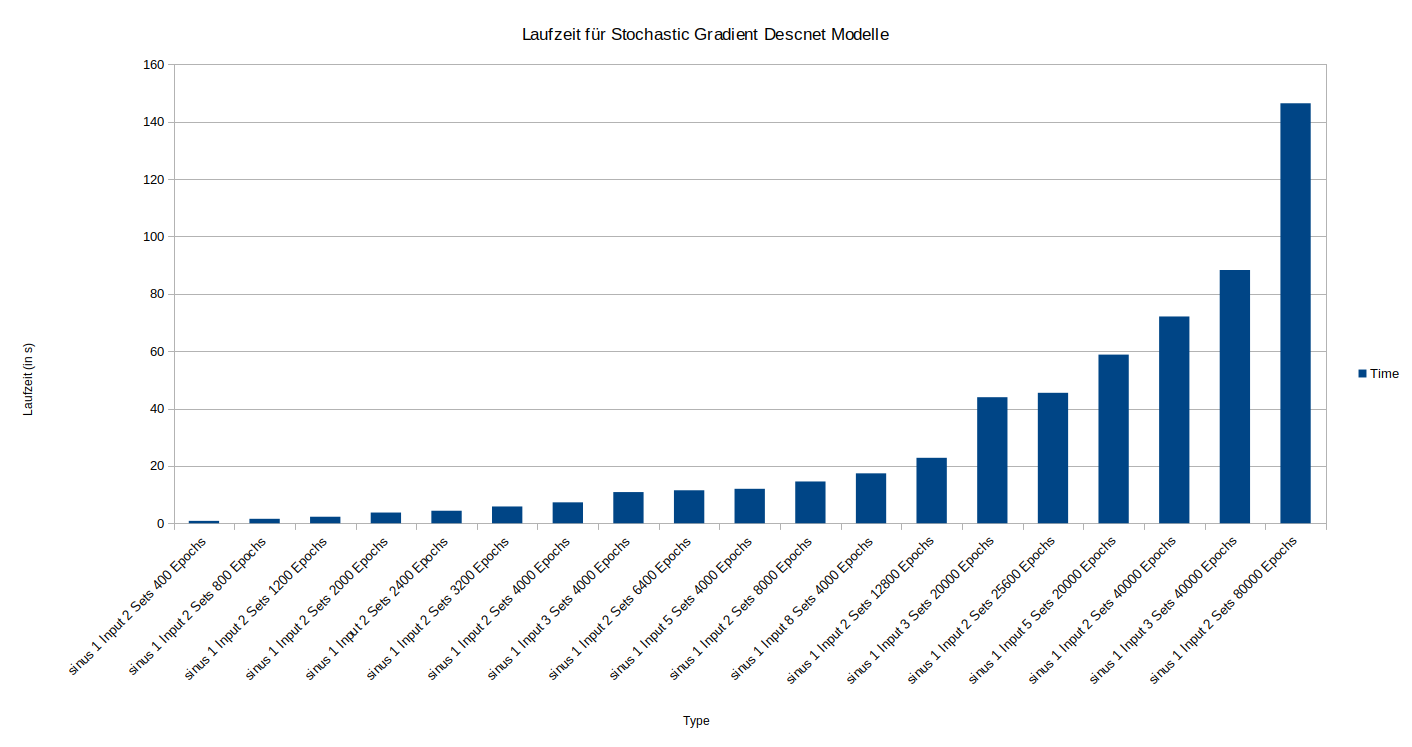
\includegraphics[angle=-90,totalheight=\textheight]{images/charts/StochasticGradientTimeSinus.png}
	\caption{Laufzeit für Stochastic-Modelle beim Erlernen der Sinusfunktion}
\end{figure}
\end{appendix}

\end{document}
